\newpage
\section{Class \tkzClass{triangle}} %(fold)


The variable \tkzVar{triangle}{T} holds a table used to store triangle objects. Its use is optional: you are free to choose another variable name, but using  \tkzVar{triangle}{T} is the recommended convention for clarity and consistency across examples and documentation.

\medskip
If you define your own table, you must initialize it manually. However, if you use the default variable  \tkzVar{triangle}{T}, the \code{init\_elements()} function will automatically clear and reset the  \tkzVar{triangle}{T} table when called.

\medskip
Each triangle object is created using the \tkzMeth{triangle}{new} method, which takes three points as input and generates all the associated geometric attributes.

\vspace{1em}

\subsection{Creating a triangle}
\label{sub:creating_a_triangle}

The \tkzClass{triangle} class is used to define triangles from three points. It automatically computes a wide range of geometric attributes associated with the triangle.

\begin{mybox}
\begin{verbatim}
T.ABC = triangle:new(z.A, z.B, z.C)
\end{verbatim}
\end{mybox}

\textbf{Short form.}

The short form \code{triangle(z.A, z.B, z.C)} is equivalent and more commonly used:

\begin{mybox}
\begin{verbatim}
T.ABC = triangle(z.A, z.B, z.C)
\end{verbatim}
\end{mybox}

\subsection{Attributes of a Triangle} %(fold)

The triangle object is created using the method \tkzMeth{triangle}{new}, for example:

\begin{center}
\code{T.ABC = triangle(z.A, z.B, z.C)}
\end{center}

(see examples: \ref{sub:alternate}, \ref{sub:apollonius_circle}, \ref{sub:excircles}). Several attributes are automatically computed and stored:

\begin{itemize}
  \item \textbf{Vertices:} The three vertices are accessible via:
  \begin{center}
    \code{T.ABC.pa}, \code{T.ABC.pb}, \code{T.ABC.pc}
  \end{center}

  \item \textbf{Sides:} The side lengths are:
  \begin{align*}
    T.ABC.a &= \text{length of } BC \\
    T.ABC.b &= \text{length of } AC \\
    T.ABC.c &= \text{length of } AB
  \end{align*}

  \item \textbf{Area:} The area is computed using Heron’s formula:
  \[
    s = \frac{a + b + c}{2}, \quad \text{Area} = \sqrt{s(s - a)(s - b)(s - c)}
  \]
  This value is stored in \code{T.ABC.area}.

  \item \textbf{Perimeter:} The perimeter is the sum of side lengths:
  \[
    P = a + b + c
  \]
  It is stored in \code{T.ABC.perimeter}.

  \item \textbf{Angles:} The internal angles $\alpha$, $\beta$, and $\gamma$ (at $A$, $B$, and $C$ respectively) are computed using the law of cosines:
  \[
  \cos(\alpha) = \frac{b^2 + c^2 - a^2}{2bc}, \quad
  \cos(\beta) = \frac{a^2 + c^2 - b^2}{2ac}, \quad
  \cos(\gamma) = \frac{a^2 + b^2 - c^2}{2ab}
  \]
  They are stored in \code{T.ABC.alpha}, \code{T.ABC.beta}, and \code{T.ABC.gamma}.
\end{itemize}

These attributes define the essential geometric properties of the triangle and are used in numerous derived methods and constructions.


\bgroup
  \small
  \captionof{table}{Triangle attributes.}\label{triangle:attributes}
  \begin{tabular}{ll}
  \toprule
  \textbf{Attributes}     & \textbf{Reference}\\
  \midrule
  \tkzAttr{triangle}{pa} &[\ref{ssub:triangle_attributes_points}]\\
  \tkzAttr{triangle}{pb} & idem \\
  \tkzAttr{triangle}{pc} & idem \\
  \tkzAttr{triangle}{type} & 'triangle' \\
  \tkzAttr{triangle}{circumcenter} &  [\ref{ssub:triangle_attributes_characteristic_points}]\\
  \tkzAttr{triangle}{centroid} & idem  \\
  \tkzAttr{triangle}{incenter} & idem \\
  \tkzAttr{triangle}{orthocenter}  & idem \\
  \tkzAttr{triangle}{eulercenter} & idem \\
  \tkzAttr{triangle}{spiekercenter} & idem;  [\ref{ssub:triangle_attributes_characteristic_points}; \ref{ssub:example_apollonius_circle}]  \\
  \tkzAttr{triangle}{a}& [\ref{ssub:triangle_attributes_lengths}]  \\
  \tkzAttr{triangle}{b}& \\
  \tkzAttr{triangle}{c}&  \\
  \tkzAttr{triangle}{alpha}&[ \ref{ssub:triangle_attributes_angles}]\\
  \tkzAttr{triangle}{beta} & \\
  \tkzAttr{triangle}{gamma}& \\
  \tkzAttr{triangle}{ab}& [\ref{ssub:triangle_attributes_straight_lines}]\\
  \tkzAttr{triangle}{bc}&  \\
  \tkzAttr{triangle}{ca}&  \\
  \tkzAttr{triangle}{semiperimeter}& [\ref{ssub:triangle_attributes_lengths}] \\
  \tkzAttr{triangle}{area}&  \\
  \tkzAttr{triangle}{inradius}& [\ref{ssub:triangle_attributes_lengths}]\\
  \tkzAttr{triangle}{circumradius}& [\ref{ssub:triangle_attributes_lengths}] \\
  \bottomrule %
  \end{tabular}
  \egroup



\subsubsection{Triangle attributes: definition points}
\label{ssub:triangle_attributes_points}

Consider a triangle $ABC$. We want to construct a new triangle whose vertices are the reflections of $A$, $B$, and $C$ with respect to the midpoints of their opposite sides.

\medskip

To achieve this, we first need to determine the midpoints of the sides of triangle $ABC$. The most straightforward approach is to use the method \tkzMeth{triangle}{medial}, which returns the \textbf{medial triangle}, i.e., the triangle formed by the midpoints of $[BC]$, $[AC]$, and $[AB]$.

\medskip

Once this medial triangle is constructed, its vertices can be accessed through standard attributes:
\begin{center}
\code{T.medial.A}, \code{T.medial.B}, \code{T.medial.C}
\end{center}


Alternatively, from the last, the method \code{get()} retrieves all three vertices at once in a convenient Lua-compatible syntax.

\medskip

For a practical illustration of this method, see  the associated \code{tikzpicture} example in the documentation.

\vspace{1em}

% see help.lua for a dev code
\begin{minipage}{.5\textwidth-2cm}
\directlua{ init_elements()
  z.A = point(0, 0)
  z.B=  point(3, 0)
  z.C = point(1, 2)
  T.ABC = triangle(z.A, z.B, z.C)
  T.m = T.ABC:medial()
  z.ma, z.mb, z.mc = T.m.pa, T.m.pb, T.m.pc
  z.Ap = z.ma:symmetry(z.A)
  z.Bp = z.mb:symmetry(z.B)
  z.Cp = z.mc:symmetry(z.C)}
\begin{center}
  \begin{tikzpicture}[scale=.75]
   \tkzGetNodes
   \tkzDrawPolygons(A,B,C)
   \tkzDrawPoints(ma, mb, mc)
   \tkzDrawPoints(A, B, C, A', B', C')
   \tkzDrawSegments[dashed](A,A' B,B' C,C')
   \tkzDrawPolygons[red](A',B',C')
  \end{tikzpicture}
\end{center}
\end{minipage}
\begin{minipage}{.5\textwidth}
\begin{tkzexample}[code only]
\directlua{ init_elements()
  z.A = point(0, 0)
  z.B=  point(3, 0)
  z.C = point(1, 2)
  T.ABC = triangle(z.A, z.B, z.C)
  T.m = T.ABC:medial()
  z.ma, z.mb, z.mc = T.m.pa, T.m.pb, T.m.pc
  z.Ap = z.ma:symmetry(z.A)
  z.Bp = z.mb:symmetry(z.B)
  z.Cp = z.mc:symmetry(z.C)}
\end{tkzexample}
\end{minipage}

\subsubsection{Triangle attributes: characteristic points}
\label{ssub:triangle_attributes_characteristic_points}
The \code{tikzpicture} environment can be viewed in the documentation.

\begin{minipage}{.5\textwidth-2cm}
\directlua{
init_elements()
   z.A = point(0, 0)
   z.B = point(4, 0)
   z.C = point(1, 3)
   T.ABC = triangle(z.A, z.B, z.C)
   z.O = T.ABC.circumcenter
   z.I = T.ABC.incenter
   z.H = T.ABC.orthocenter
   z.G = T.ABC.centroid
   z.S = T.ABC.spiekercenter}
\begin{center}
  \begin{tikzpicture}
     \tkzGetNodes
     \tkzDrawPolygon(A,B,C)
     \tkzDrawPoints(A,B,C,O,G,I,H,S)
     \tkzDrawCircles(O,A)
     \tkzLabelPoints[below](A,B,O,G,I)
     \tkzLabelPoints[above](H,S)
     \tkzLabelPoints[above](C)
  \end{tikzpicture}
\end{center}
\end{minipage}
\begin{minipage}{.5\textwidth}
\begin{tkzexample}[code only]
\directlua{
 init_elements()
 z.A = point(0, 0)
 z.B = point(4, 0)
 z.C = point(1, 3)
 T.ABC = triangle(z.A, z.B, z.C)
 z.O = T.ABC.circumcenter
 z.I = T.ABC.incenter
 z.H = T.ABC.orthocenter
 z.G = T.ABC.centroid
 z.S = T.ABC.spiekercenter}
\end{tkzexample}
\end{minipage}

\subsubsection{Triangle attributes: angles} %(fold)
\label{ssub:triangle_attributes_angles}

\begin{tkzexample}[latex=.5\textwidth-2cm]
\directlua{init_elements()
  z.A = point(0,0)
  z.B = point(5,0)
  z.C = point(2,3)
  T.ABC = triangle(z.A, z.B, z.C)
  S = T.ABC.alpha + T.ABC.beta + T.ABC.gamma}
\def\wangle#1{\tkzPN[2]{%
    \tkzUseLua{math.deg(T.ABC.#1)}}}
\begin{center}
  \begin{tikzpicture}
  \tkzGetNodes
  \tkzDrawPolygons(A,B,C)
  \tkzLabelAngle(B,A,C){$\wangle{alpha}^\circ$}
  \tkzLabelAngle(C,B,A){$\wangle{beta}^\circ$}
  \tkzLabelAngle(A,C,B){$\wangle{gamma}^\circ$}
  \end{tikzpicture}
\end{center}
The sum of the angles is: \tkzUseLua{math.deg(S)}
\end{tkzexample}

\subsubsection{Triangle attributes: lengths}
\label{ssub:triangle_attributes_lengths}

You can access different lengths, in particular side lengths with:
\begin{mybox}
\begin{tkzexample}[code only]
  T.ABC = triangle(z.A, z.B, z.C)
  p = T.ABC.a + T.ABC.b +T.ABC.c % p perimeter of T
  T.ABC.a, T.ABC.b and T.ABC.c are the lengths of the opposite sides to A, B and C.
  % Other accessible lengths
  s = T.ABC.semiperimeter
  ri = T.ABC.inradius
  R = T.ABC.circumradius
  A = T.ABC.area
\end{tkzexample}
\end{mybox}

\subsubsection{Triangle attributes: straight lines}
\label{ssub:triangle_attributes_straight_lines}

Several attributes associated with triangle sides and lines simplify code writing and improve readability.

\medskip

Consider a triangle $ABC$. Suppose you want to use the midpoint of the side $[BC]$ (which can also be seen as the base of the median from $A$). There are multiple ways to construct this midpoint in Lua, but the most concise is:

\begin{center}
\code{T.bc.mid}
\end{center}


Here:
\begin{itemize}
  \item \code{T.ABC.bc} is the attribute representing the line $(BC)$,
  \item It is equivalent to writing \code{L.BC = line(z.B, z.C)},
  \item But with a triangle object already defined as \code{T.ABC}, you can write simply:
  \begin{center}
  \code{L.BC = T.ABC.bc}
  \end{center}
\end{itemize}

\medskip

This approach saves time and space in scripts involving medians, altitudes, bisectors, or projections based on triangle sides.

\vspace{1em}

\begin{tkzexample}[latex=.5\textwidth]
\directlua{
  z.A = point(0,0)
  z.B = point(5,0)
  z.C = point(2,3)
  T.ABC = triangle(z.A, z.B, z.C)
  % z.Q = midpoint(z.A, midpoint(z.B, z.C))
  z.Q = tkz.midpoint(z.A, T.ABC.bc.mid)
  % if L.BC = line(z.B,z.C)
  % z.M = L.BC.mid gives the midpoint
}
\begin{tikzpicture}
  \tkzGetNodes
  \tkzDrawPolygon(A,B,C)
  \tkzDrawLine[add = 0 and 1](A,Q)
  \tkzDrawPoints(A,B,C,Q)
  \end{tikzpicture}
\end{tkzexample}

\subsection{Methods of the class triangle} %(fold)

\bgroup
  \catcode`_=12
  \small
  \begin{minipage}{\textwidth}
  \captionof{table}{triangle methods.}\label{triangle:methods}
  \begin{tabular}{ll}
  \toprule
  \textbf{Methods} & \textbf{Reference}      \\
  \midrule
  \tkzMeth{triangle}{new}(a, b ,c) & Note\footnote{triangle(pt, pt, pt) (short form, recommended)}; [\ref{sub:creating_a_triangle}; \ref{ssub:method_triangle_new_pt_pt_pt}]  \\
  \midrule
  \textbf{Booleans}&\\
  \midrule

  \tkzMeth{triangle}{in\_out(pt)}  & [\ref{ssub:_triangle_in__out_pt}]\\

  \tkzMeth{triangle}{check\_equilateral()}&[\ref{ssub:_triangle_check__equilateral}] \\

  \tkzMeth{triangle}{check\_acutangle()} &[\ref{ssub:_triangle_check__acutangle}] \\
  \midrule

  \textbf{Reals} &\\
   \midrule
  \tkzMeth{triangle}{area()} & better T.ABC.area\\

  \tkzMeth{triangle}{barycentric\_coordinates(pt)}& [\ref{ssub:_triangle_barycentric__coordinates_pt}]\\

  \tkzMeth{triangle}{trilinear\_coordinates(pt)} & [\ref{ssub:triangle_trilinear_coordinates_pt}]\\

  \tkzMeth{triangle}{get\_angle(arg)} & [\ref{ssub:method_triangle_get_angle}] \\


  \tkzMeth{triangle}{trilinear\_to\_d} & \ref{ssub:triangle_trilinear_to_d}\\
   \midrule
   \textbf{Points} &\\
  \midrule
  \tkzMeth{triangle}{get(arg)} & [\ref{ssub:method_triangle_get}]\\

 \tkzMeth{triangle}{point(r)} & [\ref{ssub:method_triangle_point_r}]\\

\tkzMeth{triangle}{random(<'inside'>)} & [\ref{ssub:method_triangle_random_inside}]\\

  \tkzMeth{triangle}{barycentric(ka,kb,kc)} & Note \footnote{The function \code{barycenter} is used to obtain the barycentre for any number of points }\\

  \tkzMeth{triangle}{base(u,v)} & [\ref{ssub:method_triangle_base}] \\

  \tkzMeth{triangle}{trilinear(u,v,w)}  & [\ref{ssub:method_triangle_trilinear_x_y_z}] \\

  \tkzMeth{triangle}{lemoine\_point()} &  [\ref{ssub:method_line_isosceles}]\\

  \tkzMeth{triangle}{symmedian\_point()} & [\ref{ssub:method_triangle_symmedial}] \\

  \tkzMeth{triangle}{lemoine\_point()}  &  [\ref{ssub:method_triangle_symmedial}] \\

  \tkzMeth{triangle}{bevan\_point()}  &  [\ref{ssub:method_imeth_triangle_bevan_point}; \ref{ssub:methods_triangle_bevan_circle}]\\

  \tkzMeth{triangle}{mittenpunkt\_point()} &  [\ref{ssub:method_triangle_mittenpunkt}]\\

  \tkzMeth{triangle}{gergonne\_point()} & [\ref{ssub:gergonne_point}]\\

  \tkzMeth{triangle}{nagel\_point()} & [\ref{ssub:method_triangle_nagel__point}]\\

  \tkzMeth{triangle}{feuerbach\_point()} & [\ref{ssub:method_point_feuerbach}]\\

  \tkzMeth{triangle}{spieker\_center()} & [\ref{ssub:method_triangle_spieker_center}; \ref{sub:apollonius_circle_v1_with_inversion}]\\

  \tkzMeth{triangle}{projection(p)}  & [\ref{sub:euler_relation}; \ref{ssub:method_triangle_projection_pt}]\\

  \tkzMeth{triangle}{euler\_points()} &  [\ref{ssub:method_triangle_euler__points}] \\

  \tkzMeth{triangle}{nine\_points()} &  [\ref{ssub:method_triangle_nine__points}] \\

  \tkzMeth{triangle}{taylor\_points()} & See  [\ref{ssub:method_triangle_taylor__circle}] \\

  \tkzMeth{triangle}{parallelogram()} & [\ref{ssub:director_circle}]\\

  \tkzMeth{triangle}{kimberling(n)}  & See  [\ref{ssub:method_triangle_kimberling_n}]\\

  \tkzMeth{triangle}{isogonal(p)}  & See   [\ref{ssub:method_triangle_isogonal}]\\

  \tkzMeth{triangle}{macbeath\_point()(p)}  & See   [\ref{ssub:method_triangle_macbeath_point}]\\

  \tkzMeth{triangle}{poncelet\_point(p)}  & See   [\ref{ssub:method_triangle_poncelet_point}]\\

  \tkzMeth{triangle}{orthopole(L)}  & See   [\ref{ssub:method_triangle_orthopole}]\\

  \tkzMeth{triangle}{first\_fermat\_point()}  &
    See [\ref{ssub:method_triangle_first_fermat_point}] \\

  \tkzMeth{triangle}{second\_fermat\_point()}  &
  See [\ref{ssub:method_triangle_second__fermat__point}] \\

  \tkzMeth{triangle}{lamoen\_points()}  &
See [\ref{ssub:method_triangle_lamoen_points}]\\

  \tkzMeth{triangle}{soddy\_center()}  &
See [\ref{ssub:method_triangle_soddy_center}] \\

  \tkzMeth{triangle}{conway\_points()}  &
See [\ref{ssub:method_triangle_conway_points}] \\

  \tkzMeth{triangle}{kenmotu\_point()}  &
See [\ref{ssub:_triangle_kenmotu__point}] \\

  \tkzMeth{triangle}{orthic\_axis\_points()}  &
See [ \ref{ssub:method_triangle_orthic}; \ref{ssub:method_triangle_orthic_axis_points}] \\

\tkzMeth{triangle}{isodynamic\_points()} & [\ref{ssub:isodynamic_points}] \\

  \bottomrule
  \end{tabular}
  \end{minipage}
  \egroup



  \bgroup
  \catcode`_=12
  \small
  \begin{minipage}{\textwidth}
  \captionof{table}{triangle methods.}
  \begin{tabular}{ll}
  \toprule
  \textbf{Methods} & \textbf{Reference}      \\
  \midrule

\textbf{Lines} &\\
  \midrule

  \tkzMeth{triangle}{altitude(arg) } & Note
  \footnote{|z.Ha = L.AHa.pb| recovers the common point of the opposite side and altitude. The method |orthic| is usefull. If you don't need to use the triangle object several times, you can obtain a bisector or a altitude with the function |tkz.altitude(z.A, z.B, z.C)| ; [ \ref{misc}]} [\ref{ssub:method_triangle_altitude} ]\\

  \tkzMeth{triangle}{bisector(arg) }  & Note  \footnote{|_, z.b = L.Bb:get()| recovers the common point of the opposite side and bisector. If you don't need to use the triangle object several times, you can obtain a bisector  with the function |tkz.bisector(z.A, z.B, z.C)|  [\ref{misc}]};  [\ref{ssub:method_triangle_bisector}]\\

  \tkzMeth{triangle}{bisector\_ext(arg) } & [\ref{ssub:method_triangle_bisector_ext}; \ref{sub:harmonic_division_and_bisector}]\\

\tkzMeth{triangle}{mediator(arg)} & [\ref{ssub:triangle_mediator}]\\


  \tkzMeth{triangle}{symmedian\_line(arg)} & [\ref{ssub:method_imeth_triangle_symmedian__line}
; \ref{ssub:method_triangle_symmedial} ; \ref{ssub:method_line_isosceles}]\\

  \tkzMeth{triangle}{euler\_line() } &Note
  \footnote{N center of nine points circle, G centroid, H orthocenter , O circum center } ; [\ref{ssub:euler_line}
; \ref{sub:hexagram}]\\

  \tkzMeth{triangle}{antiparallel(pt,n)} & [\ref{antiparallel};\ref{sub:antiparallel_through_lemoine_point}]\\

  \tkzMeth{triangle}{steiner\_line(pt)} &[\ref{ssub:method_triangle_steiner__line}
  ] \\

  \tkzMeth{triangle}{simson\_line(pt)} &[\ref{ssub:method_triangle_simson__line}; \ref{ssub:kiepert_hyperbola}
  ] \\

  \tkzMeth{triangle}{lemoine\_axis()} &[\ref{ssub:method_triangle_lemoine__line}
  ] \\

  \tkzMeth{triangle}{brocard\_axis()} &[\ref{ssub:method_triangle_brocard__axis}] \\

  \tkzMeth{triangle}{fermat\_axis()}  & \\

  \tkzMeth{triangle}{orthic\_axis()}  & See [\ref{ssub:method_triangle_orthic_axis}]\\

  \bottomrule
  \end{tabular}
  \end{minipage}
  \egroup



\newpage
\bgroup
\catcode`_=12
\small
\begin{minipage}{\textwidth}
    \begin{tabular}{ll}
  \toprule
  \textbf{Methods} & \textbf{Comments}     \\
  \midrule
   \textbf{Circles} &\\
  \midrule
  \tkzMeth{triangle}{euler\_circle()} & Note
   \footnote{ The midpoint of each side of the triangle, the foot of each altitude, the midpoint of the line segment from each vertex of the triangle to the orthocenter.}   [\ref{ssub:method_triangle_euler_circle}]\\

  \tkzMeth{triangle}{circum\_circle()}  & [\ref{ssub:method_triangle_circum_circle}] \\

  \tkzMeth{triangle}{in\_circle()}  &
  [\ref{ssub:method_triangle_in_circle}]\\

  \tkzMeth{triangle}{ex\_circle(n)}  & [\ref{ssub:method_triangle_ex__circle}]\\

  \tkzMeth{triangle}{first\_lemoine\_circle()}    & [\ref{ssub:method_triangle_first_lemoine_circle}
; \ref{sub:first_and_second_lemoine_circles}
  ] \\

  \tkzMeth{triangle}{second\_lemoine\_circle()}  &  \ref{sub:first_and_second_lemoine_circles}
; \ref{sub:antiparallel_through_lemoine_point}] \\

  \tkzMeth{triangle}{spieker\_circle()} &  [\ref{ssub:method_triangle_spieker__circle}]\\

  \tkzMeth{triangle}{bevan\_circle()}  & [\ref{ssub:methods_triangle_bevan_circle}]\\

  \tkzMeth{triangle}{cevian\_circle()} &  [\ref{ssub:_triangle_cevian__circle_pt}
; \ref{ssub:method_triangle_cevian}]\\

  \tkzMeth{triangle}{symmedial\_circle()}  & [\ref{ssub:method_triangle_symmedial_circ}; \ref{ssub:method_triangle_symmedial}]\\

  \tkzMeth{triangle}{pedal\_circle()} &  [\ref{ssub:method_triangle_pedal}]\\

  \tkzMeth{triangle}{conway\_circle()} &  [\ref{ssub:method_triangle_conway}]\\

  \tkzMeth{triangle}{taylor\_circle()} &  [\ref{ssub:method_triangle_taylor__circle}]\\

  \tkzMeth{triangle}{kenmotu\_circle()}  & [\ref{ssub:kenmotu_circle}]\\


  \tkzMeth{triangle}{c\_c(pt)}  &  [\ref{ssub:method_triangle_c_c}]\\

  \tkzMeth{triangle}{thebault(pt)}  &  [\ref{ssub:method_triangle_c_c}]\\

  \tkzMeth{triangle}{mixtilinear\_incircle(arg)}  &  [\ref{ssub:method_triangle_mixti}]\\

  \tkzMeth{triangle}{three\_tangent\_circles} &  [\ref{ssub:method_triangle_three_tgt_c}]\\

  \tkzMeth{triangle}{adams\_circle()}  & [\ref{ssub:method_triangle_adams_circle}]\\

  \tkzMeth{triangle}{lamoen\_circle()}  &
  See [\ref{ssub:method_triangle_lamoen_points}] \\

  \tkzMeth{triangle}{soddy\_circle()}  &
  See [\ref{ssub:method_triangle_soddy_circle}] \\

  \tkzMeth{triangle}{three\_apollonius\_circles()}  &
  See [\ref{ssub:three_apollonius_circles}] \\

  \tkzMeth{triangle}{apollonius\_circle(side, EPS)}  &
  See [\ref{ssub:apollonius_circle}] \\
  \midrule

  \textbf{Triangles} &\\
  \midrule
  \tkzMeth{triangle}{orthic()}   & [\ref{ssub:method_triangle_altitude}]   \\

  \tkzMeth{triangle}{medial()} &  [\ref{ssub:method_triangle_medial} ; \ref{sub:nine_points} ; \ref{ssub:method_triangle_symmedial}]\\

  \tkzMeth{triangle}{incentral()}  &[\ref{ssub:method_incentral}] \\

  \tkzMeth{triangle}{excentral()}  &[\ref{ssub:method_triangle_excentral}; \ref{ssub:method_triangle_feuerbach} ]  \\

  \tkzMeth{triangle}{extouch()}   &[\ref{ssub:method_triangle_extouch}; \ref{sub:excircles} ] \\

  \tkzMeth{triangle}{intouch() }   &[\ref{ssub:method_triangle_intouch}; \ref{ssub:gergonne_point}]\\

  \tkzMeth{triangle}{contact() } &  contact = intouch ; [
  \ref{ssub:gergonne_point}] \\

  \tkzMeth{triangle}{tangential()} &[\ref{ssub:method_triangle_tangential}]\\

  \tkzMeth{triangle}{anti() }&  Anticomplementary [\ref{ssub:method_triangle_anti}]  \\

  \tkzMeth{triangle}{cevian(pt)} & [\ref{ssub:method_triangle_cevian}] \\

  \tkzMeth{triangle}{pedal(pt)} &[\ref{ssub:method_triangle_pedal}]\\

  \tkzMeth{triangle}{symmedial()}  &[\ref{ssub:method_triangle_symmedial}] \\

  \tkzMeth{triangle}{euler()} & [\ref{ssub:method_triangle_euler}; \ref{ssub:method_triangle_euler__points}] \\

  \tkzMeth{triangle}{lemoine()} &[\ref{ssub:method_triangle_lemoine}] \\

  \tkzMeth{triangle}{macbeath()}  & See   [\ref{ssub:method_triangle_macbeath}]\\

  \tkzMeth{triangle}{circumcevian()}  & See   [  \ref{ssub:method_triangle_circumcevian}]\\


  \midrule
   \textbf{Conics} &\\
    \tkzMeth{triangle}{kiepert\_parabola()} & [\ref{ssub:method_triangle_kiepert_parabola}] \\

   \tkzMeth{triangle}{kiepert\_hyperbola()} & [\ref{ssub:method_triangle_kiepert__hyperbola}] \\

  \tkzMeth{triangle}{steiner\_inellipse()}& [ \ref{ssub:steiner_inellipse_and_circumellipse}] \\

  \tkzMeth{triangle}{steiner\_circumellipse()} & [ \ref{ssub:steiner_inellipse_and_circumellipse}] \\

  \tkzMeth{triangle}{euler\_ellipse()}  & [\ref{ssub:euler_ellipse}]\\

  \tkzMeth{triangle}{lemoine\_ellipse()} & [\ref{ssub:method_triangle_lemoine_inellipse}]\\

  \tkzMeth{triangle}{brocard\_inellipse()}  & [\ref{ssub:method_triangle_brocard__inellipse}]\\

  \tkzMeth{triangle}{macbeath\_inellipse()}  & [\ref{ssub:method_triangle_macbeath__inellipse}]\\

  \tkzMeth{triangle}{mandart\_ellipse()}  & [\ref{ssub:method_triangle_mandart__inellipse}]\\

  \tkzMeth{triangle}{orthic\_inellipse()}  & [\ref{ssub:method_triangle_orthic__inellipse}]\\

  \tkzMeth{triangle}{reflection()}  & [See \ref{ssub:method_triangle_reflection}; \ref{ssub:method_triangle_simson__line}; \ref{ssub:method_yiu_circles}]\\


  \midrule

  \textbf{Misc.} &\\

  \tkzMeth{triangle}{square\_inscribed()}  &  [ex.(\ref{ssub:method_triangle_square__inscribed}]\\

  \bottomrule
  \end{tabular}
  \end{minipage}
  \egroup



\subsubsection{Method \tkzMeth{triangle}{new(pt, pt, pt)}}
\label{ssub:method_triangle_new_pt_pt_pt}

This method creates a triangle object from three given points, which will serve as its vertices.

\medskip

It is widely used and appears in most examples. The syntax is:

\begin{center}
\code{T.ABC = triangle(z.A, z.B, z.C)}
\end{center}


The resulting object includes many precomputed attributes such as:
\begin{itemize}
  \item \code{T.ABC.A}, \code{T.ABC.B}, \code{T.ABC.C} — the vertices,
  \item \code{T.a}, \code{T.b}, \code{T.ABC.c} — the side lengths,
  \item \code{T.alpha}, \code{T.beta}, \code{T.gamma} — the angles,
  \item \code{T.area}, \code{T.perimeter},
  \item as well as key points like the centroid, incenter, orthocenter, circumcenter, etc.
\end{itemize}


These are available as attributes, not as methods.

\vspace{1em}
\begin{mybox}
  \begin{tkzexample}[code only]
    z.A = point(1, 0)
    z.B = point(6, 2)
    z.C = point(2, 5)
    T.ABC = triangle(z.A, z.B, z.c)
  \end{tkzexample}
\end{mybox}

\subsubsection{Method \tkzMeth{triangle}{get(<i>)}}
\label{ssub:method_triangle_get}

This method performs the inverse of triangle creation: it returns the points that define the triangle object.

\medskip

From the last version, the method also accepts an optional argument~\code{i} to retrieve a specific point:
\begin{itemize}
  \item \code{T.ABC:get()} returns all three vertices in order: \code{pa}, \code{pb}, \code{pc};
  \item \code{T.ABC:get(1)} returns only the first point (\code{pa}),
  \item \code{T.ABC:get(2)} returns the second point (\code{pb}),
  \item \code{T.ABC:get(3)} returns the third point (\code{pc}).
\end{itemize}

\medskip

Each of these points is also accessible directly as an attribute:
\begin{center}
\code{T.ABC.pa}, \code{T.ABC.pb}, \code{T.ABC.pc}
\end{center}
For example:
\begin{center}
\code{T.ABC:get(2)} is equivalent to \code{T.ABC.pb}
\end{center}

\medskip

This method belongs to a general mechanism shared by all geometric objects. Its goal is to return the minimal data required to reconstruct the object.

\vspace{1em}

\begin{minipage}{.5\textwidth}
\directlua{
  z.A = point(1, 0)
  z.B = point(2, 2)
  z.C = point(0, 1)
  T.ABC = triangle(z.A, z.B, z.C)
  T.med = T.ABC:anticomplementary()
  z.Ap, z.Bp, z.Cp = T.med:get()
  xa,ya = z.Ap:get()
  % possible
  % z.Ap = T.med.pa etc.
}
\let\tul\tkzUseLua
\begin{center}
  \begin{tikzpicture}
  \tkzGetNodes
  \tkzDrawPolygon(A,B,C)
  \tkzDrawPolygon[red](A',B',C')
  \tkzDrawPoints(A,B,C,A',B',C')
  \tkzLabelPoints(A,C')
  \tkzLabelPoint[above](A'){%
         $A':(\tul{xa};\tul{ya})$}
  \tkzLabelPoints[above left](C,B')
  \tkzLabelPoints[above right](B)
  \end{tikzpicture}
\end{center}
\end{minipage}
\begin{minipage}{.5\textwidth}
\begin{tkzexample}[code only]
\directlua{
  z.A = point(1, 0)
  z.B = point(2, 2)
  z.C = point(0, 1)
  T.ABC = triangle(z.A, z.B, z.C)
  T.med = T.ABC:anticomplementary()
  z.Ap, z.Bp, z.Cp = T.med:get()
  xa,ya = z.Ap:get()}
\end{tkzexample}
\end{minipage}

%%%%%%%%%%%%%%% boolean %%%%%%%%%%%%
\subsection{The result is a boolean}


\subsubsection{Method \tkzMeth{triangle}{in\_out(pt)}}
\label{ssub:_triangle_in__out_pt}

This method tests whether a given point lies \emph{inside} the triangle.

\medskip

It takes a single argument \code{pt}, which must be a point object. The method returns a boolean:
\begin{itemize}
  \item \code{true} if the point lies strictly inside or on the boundary of the triangle;
  \item \code{false} otherwise (i.e., if the point is strictly outside).
\end{itemize}

\medskip

This function is useful for geometric conditions, filtering, or region-based constructions.

\vspace{1em}

\begin{minipage}{.5\textwidth}
\directlua{
 init_elements()
 function pos (T, pt)
    if T : in_out (pt) then return "in"
   else return "out" end
   end
  z.A = point(1, 1)
  z.B = point(8, 0)
  z.C = point(2, 5)
  z.X = point(4, 2)
  z.Y = point(5, 4)
  T.ABC = triangle(z.A, z.B, z.C)
  strX, strY = pos(T.ABC, z.X), pos(T.ABC, z.Y)}
  \begin{center}
    \begin{tikzpicture}[scale = .75]
      \tkzGetNodes
      \tkzDrawPolygons(A,B,C)
      \tkzDrawPoints(A,B,C,X,Y)
      \tkzLabelPoints(A,B)
      \tkzLabelPoints[above](C)
      \tkzLabelPoint(X){$X$ \tkzUseLua{strX}}
      \tkzLabelPoint(Y){$Y$ \tkzUseLua{strY}}
    \end{tikzpicture}
  \end{center}
\end{minipage}
\begin{minipage}{.5\textwidth}
\begin{tkzexample}[code only]
\directlua{
 init_elements()
 function pos (T, pt)
    if T : in_out (pt) then return "in"
   else return "out" end
   end
  z.A = point(1, 1)
  z.B = point(8, 0)
  z.C = point(2, 5)
  z.X = point(4, 2)
  z.Y = point(5, 4)
  T.ABC = triangle(z.A, z.B, z.C)
  strX, strY = pos(T.ABC, z.X),
               pos(T.ABC, z.Y)}
\end{tkzexample}
\end{minipage}

\subsubsection{Method \tkzMeth{triangle}{check\_equilateral()}}
\label{ssub:_triangle_check__equilateral}

This method checks whether the triangle is equilateral, i.e., whether its three sides are of equal length within a numerical tolerance.

\medskip

It returns a boolean:
\begin{itemize}
  \item \code{true} if the triangle is equilateral,
  \item \code{false} otherwise.
\end{itemize}


This check takes into account floating-point rounding and uses an internal tolerance parameter.


\begin{mybox}
\begin{verbatim}
if T.ABC:check_equilateral() then
  -- do something
end
\end{verbatim}
\end{mybox}

\vspace{1em}

\subsubsection{Method \tkzMeth{triangle}{check\_acutangle()}}
\label{ssub:_triangle_check__acutangle}

Boolean. This method tests whether the triangle is \textbf{acutangle}, i.e., if all three of its interior angles are strictly less than $90^\circ$.

\medskip

An \emph{acutangle triangle} is a triangle where:
\[
\alpha < 90^\circ, \quad \beta < 90^\circ, \quad \gamma < 90^\circ
\]


\begin{mybox}
\begin{verbatim}
if T.ABC:check_acutangle() then
  -- do something
end
\end{verbatim}
\end{mybox}


%%%%%%%%%%%%%%%%%%%%%%%%%%%%%%%%%%%%%%%%%%%%

%%%%%%%%%%%%%%%% reals %%%%%%%%%%%%

%%%%%%%%%%%%%%%%%%%%%%%%%%%%%%%%%%%%%%%%%%%%%

\subsection{The result is a real}

\subsubsection{Method \tkzMeth{triangle}{barycentric\_coordinates(pt)}}
\label{ssub:_triangle_barycentric__coordinates_pt}

This method returns the \textbf{normalized barycentric coordinates} of a point relative to the reference triangle.

\begin{mybox}
\code{x, y, z = T: barycentric\_coordinates(z.P)}
\end{mybox}

\medskip

The result is a triple \code{x, y, z} such that:
\[
x + y + z = 1
\]

\medskip

If the point lies on a side or at a vertex, one or more coordinates will be zero accordingly. This method is especially useful for checking point location, computing weighted centers, or constructing affine invariants.

\vspace{1em}
\begin{minipage}{.45\textwidth}
  \directlua{
  init_elements()
  z.A = point(0, 0)
  z.B = point(3, 0)
  z.C = point(1, 2)
  T.ABC = triangle(z.A, z.B, z.C)
  z.G = T.ABC.centroid
  xg, yg, zg = T.ABC: barycentric_coordinates(z.G)}
  \let\tul\tkzUseLua
  \begin{tikzpicture}
  \tkzGetNodes
  \tkzDrawPolygon(A,B,C)
  \tkzDrawPoints(A,B,C,G)
  \tkzLabelPoints(A,B)
  \tkzLabelPoints[above](C)
  \tkzLabelPoint[right](G){$G: (\pmpn{\tul{xg}}:\pmpn{\tul{yg}}:\pmpn{\tul{zg}})$}
  \end{tikzpicture}
\end{minipage}
\begin{minipage}{.55\textwidth}
\begin{tkzexample}[code only]
\directlua{
  init_elements()
  z.A = point(0, 0)
  z.B = point(3, 0)
  z.C = point(1, 2)
  T.ABC = triangle(z.A, z.B, z.C)
  z.G = T.ABC.centroid
  xg, yg, zg = T.ABC: barycentric_coordinates(z.G)}
\end{tkzexample}
\end{minipage}

\subsubsection{Method \tkzMeth{triangle}{trilinear\_coordinates(pt)}}
\label{ssub:triangle_trilinear_coordinates_pt}

This method returns the \textbf{trilinear coordinates} of a point relative to the reference triangle.

\medskip

Trilinear coordinates represent a point $P$ by its (signed) distances to the sides of the triangle. The triple \code{x, y, z} corresponds to the directed distances from $P$ to the sides $BC$, $AC$, and $AB$, respectively.

\begin{mybox}
\code{x, y, z = T.ABC:trilinear\_coordinates(z.P)}
\end{mybox}

\medskip

Unlike barycentric coordinates, trilinear coordinates are homogeneous, i.e., they are defined up to a nonzero scalar multiple:
\[
P = x : y : z
\]

\subsubsection{Method \tkzMeth{triangle}{get\_angle(n)}}
\label{ssub:method_triangle_get_angle}

This method returns one of the three internal angles of the triangle, based on a cyclic permutation index \code{n}.

\medskip

It must not be confused with the function \code{get\_angle(pta, ptb, ptc)}, which computes the angle at a vertex formed by any three given points.

\medskip

The triangle's vertices are assumed to be ordered in the direct (counter-clockwise) orientation. The value of \code{n} determines which angle is computed, by applying cyclic permutations to the vertex list $(A, B, C)$:

\begin{itemize}
  \item \code{n = 0} (or omitted): returns the angle $∠BAC$,
  \item \code{n = 1}: returns the angle $∠CBA$,
  \item \code{n = 2}: returns the angle $∠ACB$.
\end{itemize}

\vspace{1em}


\begin{tkzexample}[latex=7cm]
\directlua{
 z.A = point: new(0, 0)
 z.B = point: new(4, 0)
 z.C = point: new(1, 3)
 T.ABC = triangle(z.A, z.B, z.C)
 cc = T.ABC:get_angle()
 z.O = T.ABC.circumcenter
 C.OB = circle(z.O,z.B)
 z.T = C.OB:point(.2)}
\begin{center}
\begin{tikzpicture}
 \tkzGetNodes
 \tkzDrawCircle(O,A)
 \tkzDrawArc[red,->,ultra thick](O,B)(T)
 \tkzDrawLines[red](A,B A,C)
 \tkzDrawPoints(A,B,C)
 \tkzLabelPoints(A,B)
 \tkzLabelPoints(C)
 \tkzLabelPoint[right=6pt,red,thick](T){$\mathbf{+}$}
 \tkzMarkAngle[->,red](B,A,C)
 \end{tikzpicture}
\end{center}
\end{tkzexample}

\subsubsection{Method \tkzMeth{triangle}{trilinear\_to\_d}}
\label{ssub:triangle_trilinear_to_d}

\texttt{Purpose:}
Convert a trilinear triple \((x:y:z)\) into a proportional triple \((p,q,r)\) related to the perpendicular distances from a point to the triangle sides \(BC,CA,AB\).
The method uses the current triangle side lengths \(a,b,c\) and area \(\Delta\).

\medskip
\texttt{Interest:}
Trilinear coordinates are a natural system for locating points defined by geometric relations involving the sides of a triangle
(e.g., incenters, excenters, Gergonne or Nagel points, centers of conics, etc.).
Many formulas in triangle geometry are expressed in trilinears, but practical geometric constructions often require
distances to the sides or to be converted into Cartesian coordinates.
The method \tkzname{trilinear\_to\_d} provides this essential step:
\[
(x:y:z) \quad \longrightarrow \quad (p,q,r) \propto \left(\frac{x}{a}, \frac{y}{b}, \frac{z}{c}\right)
\]
This allows the use of trilinear relations directly within the computational framework of \texttt{tkz-elements}.

\medskip
\texttt{Syntax: }
\verb|p, q, r = T:trilinear_to_d(x, y, z)|

\medskip
\texttt{Arguments: }
\begin{itemize}
  \item \code{x}, \code{y}, \code{z} — real numbers representing the trilinear coordinates.
\end{itemize}

\texttt{Returns: }
\begin{itemize}
  \item \code{p}, \code{q}, \code{r} — real numbers proportional to the distances to the triangle sides.
\end{itemize}

\texttt{Definition: }
\[
p = \Delta\,\frac{x}{a}, \qquad
q = \Delta\,\frac{y}{b}, \qquad
r = \Delta\,\frac{z}{c},
\]
where \(\Delta\) is the area of the triangle computed with Heron’s formula.

\medskip
\texttt{Remarks: }
\begin{itemize}
  \item The returned values \((p,q,r)\) are proportional to the distances, not normalized.
  \item For actual distances \((d_a,d_b,d_c)\) one can use:
  \[
    \lambda = \frac{2\Delta}{ax + by + cz}, \qquad
    d_a = \lambda x,\quad d_b = \lambda y,\quad d_c = \lambda z.
  \]
\end{itemize}


%%%%%%%%%%%%%%%%%%%%%%%%%%%%%%%%%%
%%%%%%%%%%%%%% points %%%%%%%%%%%%%
%%%%%%%%%%%%%%%%%%%%%%%%%%%%%%%%%%


\subsection{The result is a point}

\subsubsection{Method \tkzMeth{triangle}{point(r)}}
\label{ssub:method_triangle_point_r}

This method is common to most classes. It places a point along the contour of the triangle, proportionally to its perimeter.

\medskip

The parameter \code{r} must be a real number between \code{0} and \code{1}, representing the fraction of the total perimeter to travel starting from the first vertex (\code{pa}) along the oriented boundary.

\begin{itemize}
  \item If \code{r = 0} or \code{r = 1}, the method returns the first point (\code{pa}).
  \item If \code{r = 0.5}, the resulting point lies halfway along the triangle’s perimeter.
\end{itemize}

\medskip

\texttt{Example: } The point $M$ divides the perimeter into two equal arcs:
\begin{center}
\code{z.M = T.ABC:point(0.5)}
\end{center}

\vspace{1em}
\begin{tkzexample}[latex=.5\textwidth]
  \directlua{
    z.A = point(1, 0)
    z.B = point(6, 2)
    z.C = point(2, 5)
    T.ABC = triangle(z.A, z.B, z.C)
    z.M = T.ABC:point(.5)}
  \begin{tikzpicture}
    \tkzGetNodes
     \tkzDrawPolygon(A,B,C)
     \tkzDrawPoints(A,B,C,M)
     \tkzLabelPoints(A,B,C,M)
     \tkzDrawSegments[red,thick](A,B B,M)
  \end{tikzpicture}
\end{tkzexample}

\subsubsection{Method \tkzMeth{triangle}{random(<'inside'>)}}
\label{ssub:method_triangle_random_inside}

This method determines either a random point on one of the sides, or an interior point using the optional \code{inside} argument.

\begin{tkzexample}[latex=.5\textwidth]
\directlua{
  init_elements()
  z.A = point(0, 0)
  z.B = point(5, 0)
  z.C = point(1, 4)
  T.ABC = triangle(z.A, z.B, z.C)
  z.Q = T.ABC:random("inside")
  z.P = T.ABC:random() }
\begin{tikzpicture}
 \tkzGetNodes
 \tkzDrawPolygons[red](A,B,C)
 \tkzDrawPoints(A,B,C,P,Q)
 \tkzLabelPoints(P,Q)
\end{tikzpicture}
\end{tkzexample}

\subsubsection{Method \tkzMeth{triangle}{barycentric(ka, kb, kc)}}
\label{ssub:_triangle_barycentric_ka_kb_kc}

This method, also available under the alias \code{barycenter}, returns the point with barycentric coordinates $(ka : kb : kc)$ with respect to the triangle.

\medskip

These coordinates are \emph{homogeneous}, meaning only the ratio between the weights matters. The computed point $P$ satisfies:
\[
P = \frac{ka \cdot A + kb \cdot B + kc \cdot C}{ka + kb + kc}
\]
where $A$, $B$, and $C$ are the triangle's vertices.

\medskip

This method is widely used internally, notably by the \code{kimberling()} method to define classical triangle centers such as the centroid, incenter, symmedian point, etc.


\vspace{1em}

\begin{tkzexample}[latex=.5\textwidth]
\directlua{
  z.A = point(1, 0)
  z.B = point(6, 2)
  z.C = point(2, 5)
  T.ABC = triangle(z.A, z.B, z.C)
  z.P = T.ABC:barycentric(1, 1, 1)}
\begin{tikzpicture}[scale=.75]
\tkzGetNodes
\tkzDrawPolygon(A,B,C)
\tkzDrawPoint(P)
\tkzLabelPoints(A,B,P)
\tkzLabelPoints[above](C)
\end{tikzpicture}
\end{tkzexample}

\subsubsection{Method \tkzMeth{triangle}{trilinear(x, y, z)}}
\label{ssub:method_triangle_trilinear_x_y_z}

This method determines a point $P$ given its trilinear coordinates relative to a reference triangle $ABC$.

\medskip

Trilinear coordinates are defined as an ordered triple $(x, y, z)$ that is proportional to the directed distances from the point $P$ to the sides $BC$, $AC$, and $AB$ respectively.

\medskip

These coordinates are \textbf{homogeneous}, meaning they are only defined up to a nonzero scalar multiple. The point $P$ lies at the intersection of the cevians corresponding to these ratios.

\medskip

Trilinear coordinates were introduced by Plücker in 1835 and remain a fundamental tool in triangle geometry.
\begin{flushright}
\small
\href{https://mathworld.wolfram.com/TrilinearCoordinates.html}{Weisstein, Eric W. "Trilinear Coordinates." MathWorld.}
\end{flushright}

\vspace{1em}
\begin{tkzexample}[latex=.5\textwidth]
\directlua{
 init_elements()
 z.A = point(0, 0)
 z.B = point(4, 0)
 z.C = point(4, 3)
 T.ABC = triangle(z.A, z.B, z.C)
 a = T.ABC.a
 b = T.ABC.b
 c = T.ABC.c
 z.Gp = T.ABC:trilinear(b * c, a * c, a * b)
 z.G = T.ABC:barycentric(1, 1, 1)}
\begin{center}
  \begin{tikzpicture}
  \tkzGetNodes
  \tkzDrawPolygon(A,B,C)
  \tkzDrawPoints(A,B,C,G',G)
  \tkzLabelPoints(A,B,G')
  \tkzLabelPoints[above](C,G)
  \end{tikzpicture}
\end{center}
\end{tkzexample}

\subsubsection{Method \tkzMeth{triangle}{base}} %(fold)
\label{ssub:method_triangle_base}

This method computes a point defined as a linear combination of two sides of the triangle, based at the first vertex.

\medskip

Given a triangle $ABC$, the method defines a point $D$ by:
\[
\overrightarrow{AD} = \lambda \cdot \overrightarrow{AB} + \mu \cdot \overrightarrow{AC}
\]
where $\lambda$ and $\mu$ are real coefficients passed as arguments.

\medskip

\texttt{Example:} If both coefficients are \code{1}, then:
\[
\overrightarrow{AD} = \overrightarrow{AB} + \overrightarrow{AC}
\]
This yields a point located "beyond" $A$ in the direction formed by adding the two side vectors.

\begin{mybox}
\code{z.D = T.ABC:base(1,1)}
\end{mybox}

\vspace{1em}

\begin{tkzexample}[latex=.5\textwidth]
\directlua{
 init_elements()
 z.A = point(1, 1)
 z.B = point(8, 0)
 z.C = point(0, 5)
 z.X = point(2, 2)
 T.ABC = triangle(z.A, z.B, z.C)
 z.D = T.ABC:base(1, 1)
 z.E = T.ABC:base(.5, 1)}
\begin{center}
\begin{tikzpicture}[scale=.75]
     \tkzGetNodes
     \tkzDrawPolygons(A,B,D,C A,B,E,C)
     \tkzDrawPoints(A,B,C,D,E)
     \tkzLabelPoints(A,B)
     \tkzLabelPoints[above](C,D,E)
\end{tikzpicture}
\end{center}
\end{tkzexample}

\subsubsection{Method \tkzMeth{triangle}{kimberling(n)}}
\label{ssub:method_triangle_kimberling_n}

This method returns the triangle center corresponding to the Kimberling number~\code{n}.

\medskip

The enumeration of triangle centers was established by American mathematician Clark Kimberling in his \textit{Encyclopedia of Triangle Centers}, available online from the University of Evansville:
\begin{center}
\href{http://faculty.evansville.edu/ck6/encyclopedia/ETC.html}{faculty.evansville.edu/ck6/encyclopedia/ETC.html}
\end{center}


Each remarkable triangle center is assigned a unique index $X_{(n)}$. For example, the centroid is $X_{(2)}$, and the orthocenter is $X_{(4)}$.

\medskip

Only a selection of centers is currently implemented in this method. The accessible Kimberling numbers are:
\begin{multicols}{2}
\begin{itemize}
  \item $X_{(1)}$: incenter
  \item $X_{(2)}$: centroid
  \item $X_{(3)}$: circumcenter
  \item $X_{(4)}$: orthocenter
  \item $X_{(5)}$: nine-point center
  \item $X_{(6)}$: symmedian (Lemoine) point
  \item $X_{(7)}$: Gergonne point
  \item $X_{(8)}$: Nagel point
  \item $X_{(9)}$: Mittenpunkt
  \item $X_{(10)}$: Spieker center
  \item $X_{(11)}$: Feuerbach point
  \item $X_{(13)}$: First Fermat point
  \item $X_{(14)}$: Second Fermat point
  \item $X_{(19)}$: Clawson point
  \item $X_{(20)}$: de Longchamps point
  \item $X_{(55)}$, $X_{(56)}$, $X_{(110)}$, $X_{(111)}$, $X_{(115)}$
  \item $X_{(175)}$, $X_{(176)}$, $X_{(213)}$, $X_{(371)}$
\end{itemize}
\end{multicols}


\texttt{Example:}
\begin{mybox}
\code{z.G = T.ABC:kimberling(2)} \quad --> the centroid $X_{(2)}$
\end{mybox}

\vspace{1em}

\begin{tkzexample}[latex=.5\textwidth]
\directlua{
 init_elements()
 z.B = point(0, 0)
 z.C = point(4, 0)
 z.A = point(1, 3.2)
 T.ABC = triangle(z.A, z.B, z.C)
 z.H = T.ABC:kimberling(4)
 z.O = T.ABC:kimberling(3)
 L.euler = line(z.O, z.H)
 z.F = T.ABC:kimberling(110)
 kiepert = conic(z.F,L.euler,1)
 curve = kiepert:points(-4, 4, 50)
 z.ea, z.eb = L.euler:get() }
\begin{center}
\begin{tikzpicture}[scale=.8]
  \tkzGetNodes
  \tkzDrawLines[cyan,
     add= .5 and .5](A,C A,B A,C)
  \tkzDrawPolygon[cyan](A,B,C)
  \tkzDrawCoordinates[smooth,red](curve)
  \tkzDrawLines[red,add= .5 and .5](ea,eb)
  \tkzDrawPoints(A,B,C,F,O,H)
  \tkzLabelPoints(A,B,C,F,O,H)
\end{tikzpicture}
\end{center}
\end{tkzexample}

\subsubsection{Method \tkzMeth{triangle}{isogonal(pt)}} %(fold)
\label{ssub:method_triangle_isogonal}

This method returns the \textbf{isogonal conjugate} of a point~\code{pt} with respect to a triangle~$ABC$.

\medskip

The isogonal conjugate $Y$ of a point $X$ is defined as the common point of the three lines obtained by reflecting the lines $AX$, $BX$, and $CX$ across the respective internal angle bisectors at $A$, $B$, and $C$.

\medskip

An alternative but equivalent construction — and the one used in this method — consists in:
\begin{itemize}
  \item reflecting point $X$ across each side of the triangle,
  \item constructing the circle through the three reflected points,
  \item returning the center of this circle.
\end{itemize}

\medskip

\textbf{Validation:} Using this method, you can verify that the isogonal conjugate of the orthocenter is indeed the circumcenter of triangle $ABC$.

\medskip

\textbf{Geometric remark:} If a point $M$ lies on the circumcircle, then the isogonal conjugates of the points on the tangent line at $M$ trace a parabola that passes through the three vertices of the triangle. This elegant but subtle configuration highlights the dynamic complexity of isogonal mappings:
\begin{itemize}
  \item the vertices of the triangle are the conjugates of the tangent's intersection points with the triangle’s sides;
  \item points near $M$ on the tangent map to conjugates that tend toward infinity.
\end{itemize}

\medskip

In the accompanying example, $x$ is the intersection of the tangent with side $AC$, and $x'$ is a nearby point chosen to observe the behavior of its isogonal conjugate $y'$.

\vspace{1em}

 \begin{tkzexample}[latex = 6cm]
\directlua{
  z.a = point(0, 0)
  z.b = point(4, 0)
  z.c = point(1, 4)
  T.abc = triangle(z.a, z.b, z.c)
  z.H = T.abc.orthocenter
  z.O = T.abc:isogonal(z.H)
  z.I = T.abc.incenter
  C.Oa = circle(z.O, z.a)
  z.M = C.Oa:point(0.45)
  Ta = C.Oa:tangent_at(z.M)
  z.u = Ta.pb
  z.v = Ta.pa
  z.x = intersection(Ta,T.abc.ca)
  z.y = T.abc:isogonal(z.x)
  L.Mx = line(z.M,z.x)
  z.xp = L.Mx:point(0.9)
  z.yp = T.abc:isogonal(z.xp)
  PA.points = path()
  for t = 1.5, 50, 1/10 do
    local x = Ta:point(t)
    local y = T.abc:isogonal(x)
    PA.points:add_point(y)
  end
  for t = -55, 0.2, 1/10 do
    local x = Ta:point(t)
    local y = T.abc:isogonal(x)
   PA.points:add_point(y)  end}
\begin{center}
  \begin{tikzpicture}[scale=.75]
     \tkzGetNodes
     \tkzDrawPolygon(a,b,c)
     \tkzDrawCoordinates[smooth,red,thick](PA.points)
     \tkzDrawLines[add =.1 and .1](x,v a,b b,c a,x)
     \tkzDrawPoints(a,b,c,H,M,x,y,H,O,x',y')
     \tkzLabelPoints(a,b,M,H,O)
     \tkzLabelPoints[above](c,x,y,x',y')
     \tkzDrawCircles(O,a)
  \end{tikzpicture}
\end{center}
 \end{tkzexample}

\subsubsection{Method \tkzMeth{triangle}{bevan\_point()}}
\label{ssub:method_imeth_triangle_bevan_point}
The Bevan point of a triangle  is the circumcenter of the excentral triangle.

\begin{tkzexample}[latex=.5\textwidth]
  \directlua{
   init_elements()
   z.A = point(1, 1)
   z.B = point(6, 0)
   z.C = point(2, 4)
   T.ABC = triangle(z.A, z.B, z.C)
   T.exc = T.ABC:excentral()
   z.J_a, z.J_b, z.J_c = T.exc:get()
   z.c = T.ABC:bevan_point()}
  \begin{tikzpicture}[scale=.45]
    \tkzGetNodes
    \tkzDrawPolygons(A,B,C)
    \tkzDrawCircle(c,J_a)
    \tkzDrawPoints(A,B,C,c,J_a,J_b,J_c)
    \tkzLabelPoints(A,B,c,J_c)
    \tkzLabelPoints[above](C,J_a)
    \tkzLabelPoints[left](J_b)
  \end{tikzpicture}
\end{tkzexample}

\subsubsection{Method \tkzMeth{triangle}{excenter}(pt)}
\label{ssub:method_triangle_excenter_pt}
Since the argument is one of the triangle's vertices, this method returns the center of the corresponding exinscribed circle.

\subsubsection{Method \tkzMeth{triangle}{projection}(pt)}
\label{ssub:method_triangle_projection_pt}

This method returns the three orthogonal projections of a point onto the sides of the triangle.

\medskip

Given a triangle $ABC$ and a point $P$, the method computes the feet of the perpendiculars dropped from $P$ to each of the sides $[BC]$, $[AC]$, and $[AB]$.

\medskip

The result consists of three points, which can be retrieved as follows:
\begin{mybox}
\code{z.D, z.E, z.F = T.ABC:projection(z.P)}
\end{mybox}
where:
\begin{itemize}
  \item \code{z.D} is the projection onto $BC$,
  \item \code{z.E} onto $AC$,
  \item \code{z.F} onto $AB$.
\end{itemize}

\medskip

This method is useful, for example, in constructing the pedal triangle of a point with respect to a triangle.

\vspace{1em}


\begin{tkzexample}[latex = 7cm]
  \directlua{
  z.A = point(0, 0)
  z.B = point(5, 0)
  z.C = point(-.4 , 4)
  T.ABC = triangle(z.A, z.B, z.C)
  z.I = T.ABC.incenter
  z.a,
  z.b,
  z.c = T.ABC:projection(z.I)
  z.J = T.ABC:excenter(z.C)
  z.X,
  z.Y,
  z.Z = T.ABC:projection(z.J)}
  \begin{center}
    \begin{tikzpicture}[scale=.75]
    \tkzGetNodes
    \tkzDrawPolygon(A,B,C)
    \tkzDrawArc[blue](J,X)(Y)
    \tkzDrawCircle[red](I,a)
    \tkzDrawSegments[blue](J,X J,Y J,Z C,Y C,X)
    \tkzDrawSegments[red](I,a I,b I,c)
    \tkzDrawSegments[cyan,dashed](C,J)
    \tkzDrawPoints(A,B,C,I,a,b,c,J,X,Y,Z)
    \tkzLabelPoints(J,c)
    \tkzLabelPoints[right](I,X)
    \tkzLabelPoints[above](B,Z,a)
    \tkzLabelPoints[left](A,Y,b,C)
    \tkzMarkRightAngles[fill=blue!20,
       opacity=.4](A,Z,J A,Y,J J,X,B)
       \tkzMarkRightAngles[fill=red!20,
          opacity=.4](A,b,I A,c,I I,a,B)
    \end{tikzpicture}
    \end{center}
\end{tkzexample}

\subsubsection{Method \tkzMeth{triangle}{parallelogram()}}
\label{ssub:method_triangle_parallelogram}
Complete a triangle as a parallelogram. If \code{z.D = T.ABC:parallelogram()} then  $ABCD$ is a parallelogram.

\subsubsection{Method \tkzMeth{triangle}{mittenpunkt}} %(fold)
\label{ssub:method_triangle_mittenpunkt}

This method returns the \textbf{Mittenpunkt} of the triangle, also known as the \emph{middlespoint}.

\medskip

The Mittenpunkt is defined as the \emph{symmedian point of the excentral triangle}, i.e., the point of intersection of the lines joining each excenter to the midpoint of the corresponding side of the original triangle.

\medskip

It is a notable triangle center, designated as $X_{(9)}$ in Kimberling’s classification.
\begin{flushright}
\small
\href{https://mathworld.wolfram.com/Mittenpunkt.html}{Weisstein, Eric W. "Mittenpunkt." MathWorld.}
\end{flushright}

\vspace{1em}

\begin{minipage}{.5\textwidth}
\directlua{
 init_elements()
 z.A = point(0, 0)
 z.B = point(6, 0)
 z.C = point(4, 6)
 T.ABC = triangle(z.A, z.B, z.C)
 z.Ma,
 z.Mb,
 z.Mc = T.ABC:medial():get()
 z.Ia, z.Ib, z.Ic = T.ABC:excentral():get()
 z.Mi = T.ABC:mittenpunkt_point()
 T.int = T.ABC:extouch()
 z.Ta, z.Tb,
 z.Tc = T.int:get()}
\begin{center}
\begin{tikzpicture}[scale=.5]
 \tkzGetNodes
 \tkzDrawPolygons[](A,B,C Ma,Mb,Mc)
 \tkzDrawPoints(Ma,Mb,Mc,Ia,Ib,Ic)
 \tkzDrawPoints[red](Ta,Tb,Tc)
 \tkzLabelPoints[below](Ib)
 \tkzLabelPoints[above left](Ia,Ic)
 \tkzClipBB
 \tkzDrawLines[add=0 and 1](Ia,Ma Ib,Mb Ic,Mc)
 \tkzDrawLines[add=1 and 1](A,B A,C B,C)
 \tkzDrawCircles[red](Ia,Ta Ib,Tb Ic,Tc)
 \tkzDrawPoints(B,C,A,Mi) %
 \tkzLabelPoints(B,A)
 \tkzLabelPoints[above](C,Mi)
\end{tikzpicture}
\end{center}
\end{minipage}
\begin{minipage}{.5\textwidth}
\begin{tkzexample}[code only]
\directlua{
 init_elements()
 z.A = point(0, 0)
 z.B = point(6, 0)
 z.C = point(4, 6)
 T.ABC = triangle(z.A, z.B, z.C)
 z.Ma,
 z.Mb,
 z.Mc = T.ABC:medial():get()
 z.Ia, z.Ib, z.Ic = T.ABC:excentral():get()
 z.Mi = T.ABC:mittenpunkt_point()
 T.int = T.ABC:extouch()
 z.Ta, z.Tb,
 z.Tc = T.int:get()}
\end{tkzexample}
\end{minipage}

\subsubsection{Method \tkzMeth{triangle}{gergonne\_point()}} %(fold)
\label{ssub:gergonne_point}

This method returns the \textbf{Gergonne point} of the triangle, denoted $X_{(7)}$ in Kimberling’s classification.

\medskip

The Gergonne point is the common point of the lines connecting each vertex of the triangle to the point of contact of the incircle with the opposite side.

\medskip

In this example, the method is often combined with:
\begin{itemize}
  \item \tkzMeth{triangle}{intouch} – to get the contact triangle (also called the intouch triangle),
  \item \tkzMeth{triangle}{contact} – to retrieve the three contact points individually.
\end{itemize}

\medskip

These contact points are the feet of the perpendiculars from the incenter to each side, i.e., the tangency points of the incircle with the triangle’s sides.
\begin{flushright}
\small
\href{https://mathworld.wolfram.com/GergonnePoint.html}{Weisstein, Eric W. "Gergonne Point." MathWorld.}
\end{flushright}

\vspace{1em}

\begin{minipage}{.5\textwidth}
\directlua{
  init_elements()
  z.a = point(1,0)
  z.b = point(6,2)
  z.c = point(2,5)
  T.abc = triangle(z.a, z.b, z.c)
  z.g = T.abc:gergonne_point()
  z.i = T.abc.incenter
  z.ta, z.tb, z.tc = T.abc:intouch():get()}
\begin{center}
  \begin{tikzpicture}[scale=.8]
  \tkzGetNodes
  \tkzDrawPolygons(a,b,c)
  \tkzDrawSegments(a,ta b,tb c,tc)
  \tkzDrawCircle(i,ta)
  \tkzDrawPoints(a,b,c,g,ta,tb,tc)
  \tkzLabelPoints(a,b,tc)
  \tkzLabelPoints[above](c,ta)
  \tkzLabelPoints[above left](tb)
  \end{tikzpicture}
\end{center}
\end{minipage}
\begin{minipage}{.5\textwidth}
\begin{tkzexample}[code only]
\directlua{
  init_elements()
  z.a = point(1,0)
  z.b = point(6,2)
  z.c = point(2,5)
  T.abc = triangle(z.a, z.b, z.c)
  z.g = T.abc:gergonne_point()
  z.i = T.abc.incenter
  z.ta, z.tb, z.tc = T.abc:intouch():get()}
\end{tkzexample}
\end{minipage}

\subsubsection{Method \tkzMeth{triangle}{Nagel\_point}} %(fold)
\label{ssub:method_triangle_nagel__point}

Let $E_a$ be the point at which the $J_a$-excircle meets the side $(BC)$ of a triangle $ABC$, and define $E_b$ and $E_c$ similarly. Then the lines $A,E_a$, $B,E_b$ and $C,E_c$ concur in the Nagel point  $Na$.

\begin{minipage}{.5\textwidth}
\directlua{
  init_elements()
  z.A = point(0, 0)
  z.B = point(3.6, 0)
  z.C = point(2.8, 4)
  T.ABC = triangle(z.A, z.B, z.C)
  z.Na = T.ABC:nagel_point()
  z.J_a, z.J_b,
  z.J_c = T.ABC:excentral():get()
  z.E_a, z.E_b,
  z.E_c = T.ABC:extouch():get()}

\begin{center}
\begin{tikzpicture}[scale = .7]
  \tkzGetNodes
  \tkzInit[xmin=-1,xmax=7,ymin=-1,ymax=5]
  \tkzClip
  \tkzDrawPoints(A,B,C)
  \tkzDrawPoints[red,size=2](J_a,J_b,J_c)
  \tkzClipBB
  \tkzDrawLines[add=1.75 and 1.75,teal](A,B A,C B,C)
  \tkzDrawCircles(J_a,E_a J_b,E_b J_c,E_c)
  \tkzDrawSegments[dashed,gray](J_a,E_a J_b,E_b J_c,E_c)
  \tkzDrawSegments[orange](A,E_a B,E_b C,E_c)
  \tkzDrawPoints[red,size=2](Na,E_a,E_b,E_c)
  \tkzLabelPoints(A,B,Na)
  \tkzLabelPoints(E_c,J_a,J_b,J_c)
  \tkzLabelPoints[above](E_a,E_b,C)
\end{tikzpicture}
\end{center}
\end{minipage}
\begin{minipage}{.5\textwidth}
\begin{tkzexample}[code only]
\directlua{
  init_elements()
  z.A = point(0, 0)
  z.B = point(3.6, 0)
  z.C = point(2.8, 4)
  T.ABC = triangle(z.A, z.B, z.C)
  z.Na = T.ABC:nagel_point()
  z.J_a, z.J_b,
  z.J_c = T.ABC:excentral():get()
  z.E_a, z.E_b,
  z.E_c = T.ABC:extouch():get()}
\end{tkzexample}
\end{minipage}

\subsubsection{Method \tkzMeth{triangle}{feuerbach\_point()}} %(fold)
\label{ssub:method_point_feuerbach}

This method returns the \textbf{Feuerbach point} of the triangle, designated as $X_{(11)}$ in Kimberling’s classification.

\medskip

The Feuerbach point $F$ is the unique point where the triangle’s \emph{incircle} and \emph{nine-point circle} are tangent to each other.

\medskip

In addition, the three \emph{excircles} of the triangle are each tangent to the nine-point circle. These three points of tangency define what is called the \textbf{Feuerbach triangle}, whose vertices are often denoted $F_a$, $F_b$, and $F_c$.

\medskip

This construction reveals a remarkable configuration of internal and external circle tangency with the nine-point circle.
\begin{flushright}
\small
\href{https://mathworld.wolfram.com/FeuerbachPoint.html}{Weisstein, Eric W. "Feuerbach Point." MathWorld.}
\end{flushright}

\vspace{1em}


\vspace{1em}
\begin{minipage}{.5\textwidth}
\directlua{
 z.A = point(0, 0)
 z.B = point(6, 0)
 z.C = point(0.8, 4)
 T.ABC = triangle(z.A, z.B, z.C)
 z.N = T.ABC.eulercenter
 z.Fa, z.Fb,
 z.Fc = T.ABC:feuerbach():get()
 z.F =  T.ABC:feuerbach_point()
 z.Ja, z.Jb,
 z.Jc = T.ABC:excentral():get()
 z.I = T.ABC.incenter}
\begin{tikzpicture}
  \tkzGetNodes
  \tkzInit[xmin=-1,xmax=7,ymin=-1,ymax=5]
  \tkzClip
  \tkzDrawPoints(Ja,Jb,Jc)
  \tkzFillCircles[green!30,,opacity=.5](N,Fa)
  \tkzFillCircles[lightgray,,opacity=.5](I,F)
  \tkzDrawLines[add=3 and 3](A,B A,C B,C)
  \tkzDrawCircles(Ja,Fa Jb,Fb Jc,Fc N,Fa N,F I,F)
  \tkzDrawPoints(A,B,C,F,Fa,Fb,Fc,N)
  \tkzLabelPoints(I,N,A,B)
  \tkzLabelPoints[above](Fa,Fc,F,I)
  \tkzLabelPoints[left](Fb,C)
\end{tikzpicture}
\end{minipage}
\begin{minipage}{.5\textwidth}
\begin{tkzexample}[code only]
\directlua{
 z.A = point(0, 0)
 z.B = point(6, 0)
 z.C = point(0.8, 4)
 T.ABC = triangle(z.A, z.B, z.C)
 z.N = T.ABC.eulercenter
 z.Fa, z.Fb,
 z.Fc = T.ABC:feuerbach():get()
 z.F =  T.ABC:feuerbach_point()
 z.Ja, z.Jb,
 z.Jc = T.ABC:excentral():get()
 z.I = T.ABC.incenter}
\end{tkzexample}
\end{minipage}

\subsubsection{Method \tkzMeth{triangle}{symmedian\_point()}}
\label{ssub:method_triangle_lemoine_point}

This method returns the \textbf{symmedian point} $K$ of the triangle, also known as the \emph{Lemoine point} (in English and French literature) or the \emph{Grebe point} (in German).

\medskip

The symmedian point is the point of concurrence of the triangle’s three \textbf{symmedians}, which are the isogonal conjugates of the medians. In other words, $K$ is the \textbf{isogonal conjugate} of the centroid $G$.

\medskip

You can also use the aliases \code{lemoine\_point} or \code{grebe\_point} to call this method.

\medskip

A beautiful geometric property of the Lemoine point is the following:
\textit{The antiparallels to the triangle’s sides passing through the symmedian point intersect the sides in six points that all lie on a same circle} — this is known as the \textbf{first Lemoine circle}.
\begin{flushright}
\small
\href{https://mathworld.wolfram.com/SymmedianPoint.html}{Weisstein, Eric W. "Symmedian Point." MathWorld.}
\end{flushright}
\label{sub:antiparallel_through_lemoine_point}

\vspace{1em}
\begin{minipage}{.5\textwidth}
\directlua{
 init_elements()
 z.a = point(0, 0)
 z.b = point(5, 0)
 z.c = point(1, 4)
 T.abc = triangle(z.a, z.b, z.c)
 z.L = T.abc:lemoine_point()
 L.anti = T.abc:antiparallel(z.L, 0)
 z.x_0, z.x_1 =L.anti:get()
 L.anti = T.abc:antiparallel(z.L, 1)
 z.y_0, z.y_1 = L.anti:get()
 L.anti = T.abc:antiparallel(z.L, 2)
 z.z_0, z.z_1 = L.anti:get()}
\begin{center}
\begin{tikzpicture}
  \tkzGetNodes
  \tkzDrawPolygons(a,b,c)
  \tkzDrawPoints(a,b,c,L,x_0,x_1,y_0,y_1,z_0,z_1)
  \tkzLabelPoints(a,b)
  \tkzLabelPoints[above](L,c)
  \tkzDrawSegments(x_0,x_1 y_0,y_1 z_0,z_1)
  \tkzDrawCircle(L,x_0)
\end{tikzpicture}
\end{center}
\end{minipage}
\begin{minipage}{.5\textwidth}
\begin{tkzexample}[code only]
\directlua{
 init_elements()
 z.a = point(0, 0)
 z.b = point(5, 0)
 z.c = point(1, 4)
 T.abc = triangle(z.a, z.b, z.c)
 z.L = T.abc:lemoine_point()
 L.anti = T.abc:antiparallel(z.L, 0)
 z.x_0, z.x_1 =L.anti:get()
 L.anti = T.abc:antiparallel(z.L, 1)
 z.y_0, z.y_1 = L.anti:get()
 L.anti = T.abc:antiparallel(z.L, 2)
 z.z_0, z.z_1 = L.anti:get()}
\end{tkzexample}
\end{minipage}

\subsubsection{Method \tkzMeth{triangle}{spieker\_center}}
\label{ssub:method_triangle_spieker_center}

This method returns the \textbf{Spieker center} of the triangle, denoted $X_{(10)}$ in Kimberling’s classification.

\medskip

The Spieker center $S_p$ is the \textbf{incenter of the medial triangle} of the reference triangle $ABC$. It is also the center of the \emph{Spieker circle}, which is the incircle of that medial triangle.

\medskip

An important property is that the Spieker center is also the \textbf{center of the radical circle} of the triangle’s three \emph{excircles}. This makes it a key point in both classical triangle geometry and circle configurations.
\begin{flushright}
\small
\href{https://mathworld.wolfram.com/SpiekerCircle.html}{Weisstein, Eric W. "Spieker Circle." MathWorld.}
\end{flushright}

\vspace{1em}

\begin{tkzexample}[latex=.5\textwidth]
\directlua{
 z.A = point (0, 0)
 z.B = point (5, -0.5)
 z.C = point (2.2, 5)
 T.ABC = triangle(z.A, z.B, z.C)
 z.S = T.ABC:spieker_center()
 T.m = T.ABC:medial()
 z.ma, z.mb, z.mc = T.m:get()
 z.w = T.m.ab:projection(z.S)}
\begin{tikzpicture}
 \tkzGetNodes
 \tkzDrawPolygons(A,B,C ma,mb,mc)
 \tkzDrawCircles[red](S,w)
 \tkzDrawPoints(A,B,C,S,ma,mb,mc)
 \tkzLabelPoints(A,B,S,mc)
 \tkzLabelPoints[above](C,w)
 \tkzLabelPoints[right](ma)
 \tkzLabelPoints[left](mb)
\end{tikzpicture}
\end{tkzexample}

\subsubsection{Method \tkzMeth{triangle}{euler\_points}} %(fold)
\label{ssub:method_triangle_euler__points}

The points $a$, $b$ and $c$ are the Euler points. They are the midpoints of the segments $AH$, $BH$ and $CH$.

\begin{minipage}{.5\textwidth}
\directlua{
  init_elements()
  z.A = point(0, 0)
  z.B = point(5, 0)
  z.C = point(1, 4)
  T.ABC = triangle(z.A, z.B, z.C)
  z.N = T.ABC.eulercenter
  z.a,
  z.b,
  z.c = T.ABC:euler():get()
  z.H = T.ABC.orthocenter
  T.orthic = T.ABC:orthic()
  z.Ha,
  z.Hb,
  z.Hc = T.orthic:get()}
\begin{center}
  \begin{tikzpicture}[scale = 1.25]
   \tkzGetNodes
   \tkzDrawPolygons[red](A,B,C)
   \tkzDrawPolygons[cyan](a,b,c)
   \tkzDrawCircle[purple](N,a)
   \tkzDrawPoints(a,b,B,C,A,c,H)
   \tkzDrawSegments[red](C,Hc B,Hb A,Ha)
   \tkzLabelPoints(A,B,a,b,H)
   \tkzLabelPoints[above](c,C)
  \end{tikzpicture}
\end{center}
\end{minipage}
\begin{minipage}{.5\textwidth}
\begin{tkzexample}[code only]
\directlua{
  init_elements()
  z.A = point(0, 0)
  z.B = point(5, 0)
  z.C = point(1, 4)
  T.ABC = triangle(z.A, z.B, z.C)
  z.N = T.ABC.eulercenter
  z.a,
  z.b,
  z.c = T.ABC:euler():get()
  z.H = T.ABC.orthocenter
  T.orthic = T.ABC:orthic()
  z.Ha,
  z.Hb,
  z.Hc = T.orthic:get()}
\end{tkzexample}
\end{minipage}

\subsubsection{Method \tkzMeth{triangle}{nine\_points}} %(fold)
\label{ssub:method_triangle_nine__points}

This method returns the \textbf{nine classical points} that lie on the Euler circle (also called the nine-point circle) of a triangle.

\medskip

The returned points, in order, are:
\begin{itemize}
  \item the three midpoints of the sides of the triangle,
  \item the three feet of the altitudes,
  \item the three Euler points (i.e., the midpoints between each vertex and the orthocenter).
\end{itemize}

\medskip

These nine points lie on the same circle, whose center is the midpoint of the segment joining the orthocenter to the circumcenter.

\medskip

In the next example, we also compute the centroid (center of gravity) in two different ways:
\begin{itemize}
  \item using the \code{trilinear} method with coordinates $(1:1:1)$,
  \item using the \code{barycentric} method with weights $(1,1,1)$.
\end{itemize}

\vspace{1em}

\begin{minipage}{.5\textwidth}
\directlua{
  init_elements()
  z.A = point(0 ,0)
  z.B = point(5, 0)
  z.C = point(1, 4)
  T.ABC = triangle(z.A, z.B, z.C)
  z.N = T.ABC.eulercenter
  z.e1,
  z.e2,
  z.e3,
  z.e4,
  z.e5,
  z.e6,
  z.e7,
  z.e8,
  z.e9 = T.ABC:nine_points()
}
\begin{center}
  \begin{tikzpicture}[ scale = 1]
   \tkzGetNodes
   \tkzDrawPolygons[red](A,B,C)
   \tkzDrawCircle[purple](N,e1)
   \tkzDrawPoints(e1,e2,e3,e4,e5,e6,e7,e8,e9)
    \tkzLabelPoints(e1,e2,e3,e4,e5,e6,e7,e8,e9)
  \end{tikzpicture}
\end{center}
\end{minipage}
\begin{minipage}{.5\textwidth}
\begin{tkzexample}[code only]
\directlua{
  init_elements()
  z.A = point(0 ,0)
  z.B = point(5, 0)
  z.C = point(1, 4)
  T.ABC = triangle(z.A, z.B, z.C)
  z.N = T.ABC.eulercenter
  z.e1,
  z.e2,
  z.e3,
  z.e4,
  z.e5,
  z.e6,
  z.e7,
  z.e8,
  z.e9 = T.ABC:nine_points()}
\end{tkzexample}
\end{minipage}

\subsubsection{Method \tkzMeth{triangle}{soddy\_center}}
\label{ssub:method_triangle_soddy_center}

This method returns the \textbf{Soddy center} of the triangle.

\medskip

Given three mutually tangent circles (typically the triangle’s three \emph{inner Apollonius circles} centered at each vertex), there exist exactly two non-intersecting circles that are tangent to all three. These are called the \emph{inner} and \emph{outer Soddy circles}, and their respective centers are called the \textbf{inner} and \textbf{outer Soddy centers}.

\medskip

By default, the method returns the \emph{inner} Soddy center. A keyword option such as \code{"outer"} may be used to retrieve the second one, if implemented.

\medskip

See  section~\ref{ssub:method_triangle_euler_circle} for details about the associated Soddy circles.

\vspace{1em}

\vspace{1em}
\begin{minipage}{.5\textwidth}
  \directlua{
       init_elements()
       z.A = point(0, 0)
       z.B = point(4, 0.5)
       z.C = point(1, 3)
       T.ABC = triangle(z.A, z.B, z.C)
       z.S = T.ABC:soddy_center()
  }
\begin{tikzpicture}
\tkzGetNodes
\tkzDrawPolygon(A,B,C)
\tkzDrawPoints(A,B,C,S)
\tkzLabelPoints(A,B,S)
\tkzLabelPoints[above](C)
\end{tikzpicture}
\end{minipage}
\begin{minipage}{.5\textwidth}
\begin{tkzexample}[code only]
\directlua{
  init_elements()
  z.A = point(0, 0)
  z.B = point(4, 0.5)
  z.C = point(1, 3)
  T.ABC = triangle(z.A, z.B, z.C)
  z.S = T.ABC:soddy_center()}
\end{tkzexample}
\end{minipage}

\subsubsection{Method \tkzMeth{triangle}{conway\_points()}}
\label{ssub:method_triangle_conway_points}

This method returns the six points defined in \textbf{Conway’s circle theorem}.

\medskip

The Conway circle theorem states the following:

\begin{quote}
If the sides meeting at each vertex of a triangle are extended by the length of the opposite side, the six endpoints of the resulting three segments all lie on a common circle. This circle is called the \textbf{Conway circle} of the triangle, and its center is the \textbf{incenter} of the triangle.
\end{quote}

\medskip

The six returned points can then be used to draw this Conway circle and to verify its geometric properties.

\medskip

See  the corresponding figure in section~\ref{ssub:method_triangle_conway} for a complete illustration.
\begin{flushright}
\small
\href{https://en.wikipedia.org/wiki/Conway_circle_theorem}{Wikipedia – Conway circle theorem}
\end{flushright}

\vspace{1em}

\begin{mybox}
\begin{tkzexample}[code only]
  C.conway = T.ABC:conway_circle()
  z.w,z.t  = C.conway:get() %   % z.w = T.ABC : conway_center ()
  z.t1, z.t2, z.t3, z.t4, z.t5, z.t6 = T.ABC: onway_points()
\end{tkzexample}
\end{mybox}

\subsubsection{Method \tkzMeth{triangle}{first\_fermat\_point()}}
\label{ssub:method_triangle_first_fermat_point}
In a given triangle $ABC$ with all angles less than  120 degrees (2pi/3), the first Fermat point  is the point  which minimizes the sum of distances from A, B, and C.


\begin{tkzexample}[latex=.5\textwidth]
\directlua{
 z.A = point(1, 2)
 z.B = point(5, 1)
 z.C = point(2.5, 4)
 T.ABC = triangle(z.A, z.B, z.C)
 z.F1 = T.ABC:first_fermat_point()
 _,_,z.E = T.ABC.bc:equilateral("swap"):get()
 _,_,z.F = T.ABC.ca:equilateral("swap"):get()
 _,_,z.G = T.ABC.ab:equilateral("swap"):get()}
\begin{tikzpicture}
 \tkzGetNodes
 \tkzDrawPolygon(A,B,C)
 \tkzDrawSegments[dashed](B,E E,C C,F F,A)
 \tkzDrawSegments[dashed](A,G G,B)
 \tkzDrawSegments[dashed,red](A,E B,F C,G)
 \tkzDrawPoints(A,B,C,F1,E,F,G)
 \tkzLabelPoints[right](B,F1)
 \tkzLabelPoints[above](C,E,G)
 \tkzLabelPoints(A,F)
\end{tikzpicture}
\end{tkzexample}

\subsubsection{Method \tkzMeth{triangle}{second\_fermat\_point()}}
\label{ssub:method_triangle_second__fermat__point}
See  [\ref{ssub:method_triangle_fermat__axis}]
]

\subsubsection{Method \tkzMeth{triangle}{kenmotu\_point()}}
\label{ssub:_triangle_kenmotu__point}

This method returns the \textbf{Kenmotu point} of the triangle, also known as the \emph{congruent squares point}. It is listed as $X_{(371)}$ in Kimberling’s classification.

\medskip

The Kenmotu point is the unique point where three equal squares, each inscribed in the triangle and touching two sides, intersect at a single common point. Each square is constructed so that it fits snugly between two adjacent triangle sides.

\medskip

This triangle center is remarkable for its connection to equal-area geometric constructions and is defined purely by square congruence and tangency conditions.

\medskip

See  the illustration in section~\ref{ssub:kenmotu_circle} for a visual representation of the configuration.
\begin{flushright}
\small
\href{https://mathworld.wolfram.com/KenmotuPoint.html}{Weisstein, Eric W. "Kenmotu Point." MathWorld}
\end{flushright}

\subsubsection{Method \tkzMeth{triangle}{adams\_points()}}
\label{ssub:method_triangle_adams_points}
Given a triangle $ABC$, construct the \code{contact} triangle $T_AT_BT_C$. Now extend lines parallel to the sides of the contact triangle from the \code{Gergonne} point. These intersect the triangle $ABC$ in the six points $P, Q,  R, S, T$, and $U$. \code{C. Adams} proved in 1843 that these points are concyclic in a circle now known as the Adams' circle.
\begin{flushright}
\small
\href{ https://mathworld.wolfram.com/AdamsCircle.html}{Weisstein, Eric W. "Adams' Circle." From MathWorld--A Wolfram Web Resource.}
\end{flushright}

\subsubsection{Method \tkzMeth{triangle}{macbeath\_point}}
\label{ssub:method_triangle_macbeath_point}
The MacBeath point is the center of the cercle kimberling(264).

\begin{tkzexample}[latex=.5\textwidth]
\directlua{
init_elements()
z.A = point(.5, 3)
z.B = point(0, 0)
z.C = point(5, 0)
T.ABC = triangle(z.A, z.B, z.C)
z.MB = T.ABC:macbeath_point()
z.Xa, z.Xb,
z.Xc = T.ABC:macbeath():get()}
\begin{tikzpicture}
\tkzGetNodes
\tkzDrawPolygons(A,B,C Xa,Xb,Xc)
\tkzDrawSegments(A,Xa B,Xb C,Xc)
\tkzDrawPoints(A,B,C,MB,Xa,Xb,Xc)
\tkzLabelPoints(B,C,MB)
\tkzLabelPoints[above](A)
\end{tikzpicture}
\end{tkzexample}

\subsubsection{Method \tkzMeth{triangle}{poncelet\_point}(p)}
\label{ssub:method_triangle_poncelet_point}

If the three vertices and the $p$ point do not form a orthocentric system et no three of them are collinear. The nine-point circles of the four triangles obtained with three of the four points have one thing in common, called \tkzname{Poncelet} point.

\begin{tkzexample}[latex=.5\textwidth]
\directlua{
 init_elements()
 z.A = point(1, 1)
 z.B = point(6, 0)
 z.C = point(0, 5)
 z.X = point(2, 2)
 T.ABC = triangle(z.A, z.B, z.C)
 z.P = T.ABC:poncelet_point(z.X)
 z.I = T.ABC.eulercenter
 z.Ma, z.Mb, z.Mc = T.ABC:medial():get()
 T.ABX = triangle(z.A, z.B, z.X)
 z.I1 = T.ABX.eulercenter}
\begin{center}
\begin{tikzpicture}
  \tkzGetNodes
  \tkzDrawPolygons(A,B,C)
  \tkzDrawPoints(A,B,C,X,P)
  \tkzDrawCircles[red](I,Ma I1,Mc)
  \tkzLabelPoints(A,B)
  \tkzLabelPoints[above](C,X,P)
\end{tikzpicture}
\end{center}
\end{tkzexample}

\subsubsection{Method \tkzMeth{triangle}{orthopole}}
\label{ssub:method_triangle_orthopole}

For the definition and some properties, please refer to:
\begin{flushright}
\small
\href{ https://mathworld.wolfram.com/Orthopole.html}{Weisstein, Eric W. "Orthopole." From MathWorld--A Wolfram Web Resource.}
\end{flushright}

See the following example for the link between orthopole and Simson line: [\ref{sub:orthopole_and_simson_line}]

\begin{tkzexample}[latex=.5\textwidth]
\directlua{
 init_elements()
 z.A = point(0, 0)
 z.B = point(5, 0)
 z.C = point(1, 4)
 T.ABC = triangle(z.A, z.B, z.C)
 z.N = T.ABC.eulercenter
 z.H = T.ABC.orthocenter
 L.NH = line(z.N, z.H)
 z.P = T.ABC:orthopole(L.NH)
}
\begin{center}
 \begin{tikzpicture}
  \tkzGetNodes
  \tkzDrawPolygons[cyan](A,B,C)
  \tkzDrawLine[purple,add = 2 and 2](N,H)
  \tkzDrawPoints(A,B,C,N,H,P)
  \tkzLabelPoints(A,B,H,N)
  \tkzLabelPoints[above](C,P)
 \end{tikzpicture}
\end{center}
\end{tkzexample}

\subsubsection{Method \tkzMeth{triangle}{isodynamic\_points()}}
\label{ssub:isodynamic_points}

This method computes the two isodynamic points of a non-degenerate triangle.

\medskip

\texttt{Geometric background: }
Given a triangle $ABC$, consider the three Apollonius circles associated with its sides:
\[
\mathcal{A}_{a},\quad \mathcal{A}_{b},\quad \mathcal{A}_{c},
\]
each defined as the locus of points $M$ satisfying a ratio of distances
corresponding to the opposite sides.

A classical and fundamental property states that:

\begin{quote}
\emph{The three Apollonius circles intersect in exactly two points.
These intersections are the first and second isodynamic points of the triangle.}
\end{quote}

The first isodynamic point is symmetric to the second by reflection in the
circumcenter. Both points are isogonal conjugates of the Fermat points.

\medskip

\texttt{Description: }
The method \code{isodynamic\_points()}  returns the two common intersection points of the Applonius circles.

\medskip
\texttt{Return values: }
\begin{itemize}
  \item \code{S1} — the first isodynamic point,
  \item \code{S2} — the second isodynamic point.
\end{itemize}

\medskip
\texttt{Example: }
\begin{verbatim}
S1, S2 = T.ABC:isodynamic_points()
\end{verbatim}

Each point can then be used like any other \code{point} object in subsequent constructions.

\medskip
\texttt{Application: }

\begin{tkzexample}[vbox]
\directlua{%
z.A = point (0, 0)
z.B = point (5, 0)
z.C = point (3.5, 2)
T.ABC = triangle (z.A,  z.B, z.C)
C.ab, C.bc,
C.ca = T.ABC:three_apollonius_circles()
z.w1, z.t1 = C.ab:get()
z.w2, z.t2 = C.bc:get()
z.w3, z.t3 = C.ca:get()
z.S, z.Sp = T.ABC:isodynamic_points()
}
\begin{center}
\begin{tikzpicture}[scale=.5]
 \tkzGetNodes
 \tkzDrawLines[add = 1.5 and 1.5,
               dashed](A,B B,C C,A)
 \tkzDrawPolygons(A,B,C)
 \tkzDrawCircle[purple](O,A)
 \tkzDrawCircles[cyan](w1,t1 w2,t2 w3,t3)
 \tkzDrawLines[purple](w1,w2)
 \tkzDrawPoints(A,B,C,w1,w2,w3,S,S')
 \tkzLabelPoints(A,B,w1,w2,w3)
  \tkzLabelPoints[above](C,S,S')
\end{tikzpicture}
\end{center}
\end{tkzexample}


\subsubsection{Method \tkzMeth{triangle}{apollonius\_points(side)}}
\label{ssub:apollonius_points}

This method returns the two Apollonius division points associated with a
specified side of the triangle.

\medskip

\paragraph{Description.}
Given a triangle $ABC$ and a chosen side:

\begin{itemize}
  \item \code{"ab"} — side $AB$, ratio defined by the opposite side $c = AB$,
  \item \code{"bc"} — side $BC$, ratio defined by the opposite side $a = BC$,
  \item \code{"ca"} — side $CA$, ratio defined by the opposite side $b = CA$,
\end{itemize}

the method  returns the two
points that divide the chosen side internally and externally according to the
ratio of the adjacent sides.

\medskip
\texttt{Return values: }
Two points:
\begin{itemize}
  \item \code{P\_int} — internal division point on the chosen side,
  \item \code{P\_ext} — external division point on the chosen side.
\end{itemize}

\medskip

\texttt{Example: }
\begin{verbatim}
Pin, Pex = T.ABC:apollonius_points("ab")
\end{verbatim}

The returned objects are standard \code{point} instances usable in further
constructions.

\texttt{Application: } See [\ref{ssub:apollonius_circle}]

%%%%%%%%%%%%%%%%%%%%%%%%%%%%%%%%%%%%%%
%%%%%%%%%%%  Lines %%%%%%%%%%%
%%%%%%%%%%%%%%%%%%%%%%%%%%%%%%%%%%%%%%

\subsection{The result is a line}
\subsubsection{Method \tkzMeth{triangle}{symmedian\_line(n)}}
\label{ssub:method_imeth_triangle_symmedian__line}

This method returns one of the \textbf{symmedians} of the triangle.

\medskip

The lines $AL_a$, $BL_b$, and $CL_c$, which are the isogonal conjugates of the medians $AM_a$, $BM_b$, and $CM_c$, are called the triangle’s \textbf{symmedians}. These lines concur at a point $L$, known as the \textbf{Lemoine point} or \textbf{symmedian point}. It is the isogonal conjugate of the centroid $G$.

\medskip

The triangle $L_aL_bL_c$, formed by the intersections of the symmedians with the sides of the triangle $ABC$, is called the \textbf{symmedial triangle}. The circle circumscribed about this triangle is known as the \textbf{symmedial circle}.

\medskip

To obtain:
\begin{itemize}
  \item all three symmedians, use the method \code{symmedian()};
  \item the point of concurrency, use \code{symmedian\_point()} or \code{lemoine\_point()};
  \item only one symmedian, use \code{symmedian\_line(n)} with \(n=0\), \(1\), or \(2\), corresponding respectively to the vertices $A$, $B$, or $C$.
\end{itemize}

\medskip

In the following example, the point $L$ is the Lemoine point, and the triangle $L_aL_bL_c$ is the symmedial triangle.
\begin{flushright}
\small
\href{https://mathworld.wolfram.com/SymmedianPoint.html}{Weisstein, Eric W. "Symmedian Point." MathWorld.}
\end{flushright}

\vspace{1em}

\begin{minipage}{.55\textwidth}
\directlua{
   init_elements()
   z.A = point(0, 0)
   z.B = point(7, -1)
   z.C = point(2.6, 3)
   T.ABC = triangle(z.A, z.B, z.C)
   z.L = T.ABC:lemoine_point()
   T.SY = T.ABC:symmedial()
   T.med = T.ABC:medial()
   z.La, z.Lb, z.Lc = T.SY:get()
   z.Ma, z.Mb, z.Mc = T.med:get()
   L.Lb = T.ABC:symmedian_line(1)
  _, z.Lb = L.Lb:get()
  z.G = T.ABC.centroid
  z.Ia, z.Ib, z.Ic = T.ABC:incentral():get()
  z.I = T.ABC.incenter
}
\begin{center}
  \begin{tikzpicture}[scale =1,font=\small]
  \tkzGetNodes
  \tkzDrawPolygons(A,B,C)
  \tkzDrawPoints(A,B,C,L,La,Lb,Lc,G,Ma,Mb,Mc,Ia,Ib,Ic,I)
  \tkzDrawSegments[cyan](A,La B,Lb C,Lc)
  \tkzDrawSegments[green](A,Ma B,Mb C,Mc)
  \tkzDrawSegments[dashed,red](A,Ia B,Ib C,Ic)
  \tkzLabelPoints[above](C,La,Ia,Ma)
  \tkzLabelPoints[above=4pt](Lb)
  \tkzLabelPoints[above left=1pt](Ib)
  \tkzLabelPoints[left](Mb)
  \tkzLabelPoints(A,B,L,Lc,I,Ic,Mc,G)
  \end{tikzpicture}
\end{center}
\end{minipage}
\begin{minipage}{.45\textwidth}
\begin{tkzexample}[code only]
\directlua{
 init_elements()
 z.A = point(0, 0)
 z.B = point(6, 0)
 z.C = point(2.4, 1.8)
 T.ABC = triangle(z.A, z.B, z.C)
 z.L = T.ABC:lemoine_point()
 T.SY = T.ABC:symmedian()
 T.med = T.ABC:medial()
 z.Ka, z.Kb, z.Kc = T.SY:get()
 z.Ma, z.Mb, z.Mc = T.med:get()
 L.Kb = T.ABC:symmedian_line(1)
 _, z.Kb = L.Kb:get()
 z.G = T.ABC.centroid
 z.Ia, z.Ib,
 z.Ic = T.ABC:incentral():get()
 z.I = T.ABC.incenter}
\end{tkzexample}
\end{minipage}

\subsubsection{Method \tkzMeth{triangle}{altitude(arg)}} %(fold)
\label{ssub:method_triangle_altitude}

This method returns one of the \textbf{altitudes} of a triangle.

\medskip
There are multiple ways to access altitudes:
\begin{itemize}
  \item \tkzMeth{triangle}{orthic} returns the \textbf{orthic triangle}, whose vertices are the feet of the three altitudes.
  \item \tkzMeth{triangle}{altitude} returns a single altitude line, based on an optional argument.
\end{itemize}

\medskip
The optional argument \code{arg} determines from which vertex the altitude is dropped. It may be:
\begin{itemize}
  \item \code{nil} or \code{0} (default): returns the altitude from vertex $A$;
  \item \code{1}: returns the altitude from vertex $B$;
  \item \code{2}: returns the altitude from vertex $C$;
  \item a point equal to \code{z.A}, \code{z.B}, or \code{z.C} (the vertex of origin).
\end{itemize}

\medskip

This interface matches that of other methods such as \tkzMeth{triangle}{bisector} and \tkzMeth{triangle}{symmedian\_line}.

\vspace{1em}

\begin{minipage}{.5\textwidth}
\directlua{
  init_elements()
  z.A = point(0, 0)
  z.B = point(5, 0)
  z.C = point(2, 4)
  T.ABC = triangle(z.A, z.B, z.C)
  z.H = T.ABC.orthocenter
  L.HA = T.ABC:altitude()
  L.HC = T.ABC:altitude(z.C)
  z.Hc = L.HC.pb
  z.Ha = L.HA.pb
  z.a, z.b,
  z.c = T.ABC:orthic():get()}
  \begin{tikzpicture}
   \tkzGetNodes
   \tkzDrawPolygon(A,B,C)
   \tkzDrawPolygon[red](a,b,c)
   \tkzDrawPoints(A,B,C,H)
   \tkzDrawSegments[red](C,Hc A,Ha)
   \tkzLabelPoints(A,B,H)
   \tkzLabelPoints(Hc)
   \tkzLabelPoints[above](Ha,C)
   \tkzMarkRightAngles[fill = gray!30,
         opacity=.4](B,Hc,C A,Ha,C)
  \end{tikzpicture}
\end{minipage}
\begin{minipage}{.5\textwidth}
\begin{tkzexample}[code only]
\directlua{
  init_elements()
  z.A = point(0, 0)
  z.B = point(5, 0)
  z.C = point(2, 4)
  T.ABC = triangle(z.A, z.B, z.C)
  z.H = T.ABC.orthocenter
  L.HA = T.ABC:altitude()
  L.HC = T.ABC:altitude(z.C)
  z.Hc = L.HC.pb
  z.Ha = L.HA.pb
  z.a, z.b,
  z.c = T.ABC:orthic():get()}
\end{tkzexample}
\end{minipage}

\subsubsection{Method \tkzMeth{triangle}{bisector(arg)}} %(fold)
\label{ssub:method_triangle_bisector}

This method returns one of the three \textbf{internal angle bisectors} of a triangle.

\medskip

In many cases, it may be sufficient to compute the incenter and connect it to the triangle’s vertices, since all bisectors pass through the incenter. For example:
\begin{mybox}
\code{z.I = T.ABC.incenter}
\end{mybox}


However, the method \code{bisector(arg)} explicitly computes the intersection of the bisector with the opposite side. This is useful for constructing the \emph{incentral triangle} or other derived figures.

\medskip

If all three bisectors are needed, use the method \tkzMeth{triangle}{incentral}, which returns the \textbf{incentral triangle}, whose vertices are the feet of the internal bisectors.

\medskip

The optional argument \code{arg} controls from which vertex the bisector originates. It can be:
\begin{itemize}
  \item \code{nil} or \code{0} (default): bisector from vertex $A$;
  \item \code{1}: bisector from vertex $B$;
  \item \code{2}: bisector from vertex $C$;
  \item a point equal to one of the triangle’s vertices, such as \code{z.A}, \code{z.B}, or \code{z.C}.
\end{itemize}


This behavior is consistent with other methods like \code{altitude}, \code{symmedian\_line}, and \code{mediator}.

\vspace{1em}
\begin{minipage}{.5\textwidth}
\directlua{
  init_elements()
  z.A = point(0, 0)
  z.B = point(3, 2)
  z.C = point(2, 5)
  T.ABC = triangle(z.A, z.B, z.C)
  L.AE = T.ABC:bisector()
  z.E  = L.AE.pb
  z.F  = T.ABC:bisector(z.B).pb
  z.a, z.b, z.c = T.ABC:incentral():get()
  z.I = T.ABC.incenter}
\begin{center}
  \begin{tikzpicture}
   \tkzGetNodes
   \tkzDrawPolygon(A,B,C)
   \tkzDrawPolygon[cyan](a,b,c)
   \tkzDrawLines(A,B A,C A,E B,F)
   \tkzDrawPoints(A,B,C,a,b,c)
   \tkzMarkAngles[cyan,mark=|,size=.75](B,A,a a,A,C)
   \tkzMarkAngles[mark=||,size=.5](C,B,b b,B,A)
   \tkzDrawLines[red](A,E B,F)
   \tkzDrawPoints(A,B,C,E,F,I)
   \tkzLabelPoints(A,B,I)
   \tkzLabelPoints[above left](C,F,E)
  \end{tikzpicture}
\end{center}
\end{minipage}
\begin{minipage}{.5\textwidth}
\begin{tkzexample}[code only]
\directlua{
  init_elements()
  z.A = point(0, 0)
  z.B = point(3, 2)
  z.C = point(2, 5)
  T.ABC = triangle(z.A, z.B, z.C)
  L.AE = T.ABC:bisector()
  z.E  = L.AE.pb
  z.F  = T.ABC:bisector(z.B).pb
  z.a, z.b, z.c = T.ABC:incentral():get()
  z.I = T.ABC.incenter}
\end{tkzexample}
\end{minipage}

\subsubsection{Method \tkzMeth{triangle}{bisector\_ext(arg)}}
\label{ssub:method_triangle_bisector_ext}

This method returns an \textbf{external angle bisector} of the triangle, from a specified vertex.

\medskip

Its interface is identical to \tkzMeth{triangle}{bisector}, accepting either an index \code{n} or a vertex point (\code{z.A}, \code{z.B}, \code{z.C}). See Section~\ref{ssub:method_triangle_bisector} for usage details.

\subsubsection{Method \tkzMeth{triangle}{mediator(...)}}
\label{ssub:triangle_mediator}

This method returns the perpendicular bisector of one side of a triangle.

\texttt{Syntax: }

\begin{verbatim}
L = triangle:mediator()
L = triangle:mediator(n) n = 0, 1 or 2
L = triangle:mediator(pt) pt vertex of the triangle
\end{verbatim}

\texttt{Arguments: }

\begin{itemize}
  \item If no argument or \texttt{n = 0} is given, the bisector of side \tkzname{AB} is returned.
  \item If \texttt{n = 1}, the bisector of side \tkzname{BC} is returned.
  \item If \texttt{n = 2}, the bisector of side \tkzname{CA} is returned.
  \item If a point (\tkzname{pa}, \tkzname{pb}, \tkzname{pc}) is passed, the method returns the bisector of the side opposite to that vertex.
\end{itemize}

\texttt{Return value: }

Returns a \tkzname{line} object representing the perpendicular bisector of the selected side.

\texttt{Examples.}

\begin{mybox}
\begin{verbatim}
T = triangle(z.A, z.B, z.C)
L1 = T:mediator()        -- bisector of AB
L2 = T:mediator(1)       -- bisector of BC
L3 = T:mediator(z.C)     -- bisector of AB (since C is opposite AB)
\end{verbatim}
\end{mybox}


\begin{tkzexample}[latex=.55\textwidth]
\directlua{
  z.A = point(0, 0)
  z.B = point(3, 2)
  z.C = point(2, 5)
  T.ABC = triangle(z.A, z.B, z.C)
  L.MA  = T.ABC:mediator(z.A)
  L.MB  = T.ABC:mediator(z.B)
  L.MC  = T.ABC:mediator(z.C)
  z.ma1, z.ma2 = L.MA:get()
  z.mb1, z.mb2 = L.MB:get()
  z.mc1, z.mc2 = L.MC:get()}
\begin{center}
\begin{tikzpicture}
  \tkzGetNodes
  \tkzDrawPolygon(A,B,C)
  \tkzDrawLines[red,
  add = .25 and .25](ma1,ma2 mb1,mb2
        mc1,mc2)
  \tkzDrawPoints(A,B,C,ma1,ma2)
\end{tikzpicture}
\end{center}
\end{tkzexample}


\textbf{See also.} \tkzFct{line}{mediator}, \tkzFct{triangle}{altitude}, \tkzFct{triangle}{bisector}

\subsubsection{Method \tkzMeth{triangle}{antiparallel(arg)}}
\label{antiparallel}

This method returns an \textbf{antiparallel line} associated with a triangle and one of its angles.

Two lines, such as $(PQ)$ and $(BC)$, are said to be \textbf{antiparallel} with respect to an angle (e.g., $\angle A$) if they form equal angles (in opposite directions) with the bisector of that angle.


Useful properties of antiparallel lines:
\begin{itemize}
  \item If $(PQ)$ and $(BC)$ are antiparallel with respect to $\angle A$, then the four points $P$, $Q$, $B$, and $C$ are \textbf{concyclic}.
  \item Antiparallelism is symmetric: if $(PQ)$ is antiparallel to $(BC)$, then $(BC)$ is antiparallel to $(PQ)$.
\end{itemize}

\medskip

This method takes two arguments:
\begin{itemize}
  \item \code{pt} (mandatory): a point through which the antiparallel line will pass;
  \item \code{arg} (optional): specifies the vertex of the triangle that defines the reference angle.
\end{itemize}


The second argument \code{arg} can be:
\begin{itemize}
  \item \code{nil} or \code{0} (default): antiparallel to $BC$ w.r.t.\ angle $\widehat{A}$;
  \item \code{1}: antiparallel to $AC$ w.r.t.\ angle $\widehat{B}$;
  \item \code{2}: antiparallel to $AB$ w.r.t.\ angle $\widehat{C}$;
  \item a point equal to one of the triangle’s vertices: \code{z.A}, \code{z.B}, or \code{z.C}.
\end{itemize}

\medskip

This method is used, for example, in the construction of the symmedian point (see section~\ref{ssub:method_triangle_lemoine_point}).

\vspace{1em}
\begin{minipage}{.5\textwidth}
  \directlua{
    init_elements()
    z.B = point(0, 0)
    z.C = point(5, 0)
    z.A = point(1, 4)
    T.ABC = triangle(z.A, z.B, z.C)
    z.M = point(2, 2)
    L.anti = T.ABC:antiparallel(z.M, z.A)
    z.P, z.Q = L.anti:get()
    T.PQ = triangle(z.P, z.Q, z.B)
    z.W = T.PQ.circumcenter}
  \begin{tikzpicture}[scale=.8]
    \tkzGetNodes
    \tkzDrawPolygons(A,B,C)
    \tkzDrawPoints(A,B,C,M,P,Q)
    \tkzLabelPoints(A,B,P,Q)
    \tkzLabelPoints[above](M,C)
    \tkzDrawSegments(P,Q)
    \tkzDrawCircle(W,P)
  \end{tikzpicture}
\end{minipage}
\begin{minipage}{.5\textwidth}
\begin{tkzexample}[code only]
  \directlua{
    init_elements()
    z.B = point(0, 0)
    z.C = point(5, 0)
    z.A = point(1, 4)
    T.ABC = triangle(z.A, z.B, z.C)
    z.M = point(2, 2)
    L.anti = T.ABC:antiparallel(z.M, z.A)
    z.P, z.Q = L.anti:get()
    T.PQ = triangle(z.P, z.Q, z.B)
    z.W = T.PQ.circumcenter}
\end{tkzexample}
\end{minipage}

\subsubsection{Method  \tkzMeth{triangle}{orthic\_axis()} and \tkzMeth{triangle}{orthic\_axis\_points()}}
\label{ssub:method_triangle_orthic_axis}
\label{ssub:method_triangle_orthic_axis_points}

Let $H_AH_BH_C$ be the \textbf{orthic triangle} of a reference triangle $ABC$ (i.e., the triangle formed by the feet of the altitudes from each vertex).

\medskip

Each side of triangle $ABC$ intersects each side of triangle $H_AH_BH_C$, and the three points of intersection all lie on a common straight line. This line is known as the \textbf{orthic axis} of the triangle.

\medskip

The method \tkzMeth{triangle}{orthic\_axis()} returns this line as an object of class \code{line}.
The method \tkzMeth{triangle}{orthic\_axis\_points()} returns the three intersection points between corresponding sides of the reference triangle and the orthic triangle. These are the points $O_A$, $O_B$, and $O_C$ aligned on the orthic axis.

\medskip

This remarkable line is a classical geometric construction, often overlooked despite its elegance.

\vspace{1em}

\begin{tkzexample}[latex=.5\textwidth]
\directlua{
  z.B = point(0, 0)
  z.C = point(5, 0)
  z.A = point(.6, 3)
  T.ABC = triangle(z.A, z.B, z.C)
  z.H = T.ABC.orthocenter
  z.H_A, z.H_B,
  z.H_C  = T.ABC:orthic():get()
  L.orthic  = T.ABC:orthic_axis()
  z.Q_A, z.Q_B,
  z.Q_C = T.ABC:orthic_axis_points()}
\begin{center}
\begin{tikzpicture}
 \tkzGetNodes
 \tkzDrawPolygons[cyan](A,B,C)
 \tkzDrawLines[red](Q_C,Q_B)
 \tkzDrawSegments(A,Q_C B,Q_A A,H_A)
 \tkzDrawSegments(B,H_B C,H_C C,Q_B)
 \tkzDrawSegments[dashed](H_B,Q_C H_B,Q_A)
 \tkzDrawSegments[dashed](H_A,Q_B)
 \tkzDrawPoints(A,B,C,H_A,H_B,H_C)
 \tkzDrawPoints(H,Q_A,Q_B,Q_C)
 \tkzLabelPoints(H)
 \tkzLabelPoints(B,C,H_A)
 \tkzLabelPoints[above right](A,H_B)
 \tkzLabelPoints[left](H_C,Q_A,Q_B,Q_C)
\end{tikzpicture}
\end{center}
\end{tkzexample}


\subsubsection{Methods \tkzMeth{triangle}{euler\_line()} and \tkzMeth{triangle}{orthic\_axis()}} %(fold)
\label{ssub:euler_line}

These two methods return two fundamental lines associated with triangle geometry: the \textbf{Euler line} and the \textbf{orthic axis}.

\medskip

\textbf{Euler line} — The line on which lie several remarkable triangle centers:
\begin{itemize}
  \item the orthocenter $H$,
  \item the centroid $G$,
  \item the circumcenter $O$,
  \item the nine-point center $N$,
  \item and many others.
\end{itemize}



\medskip

\textbf{Orthic axis} — Let $h_a$, $h_b$, and $h_c$ be the vertices of the orthic triangle of triangle $ABC$. Each side of triangle $ABC$ intersects each side of the orthic triangle. The three points of intersection lie on a line called the \textbf{orthic axis}.

\begin{itemize}
  \item This line is \emph{perpendicular} to the Euler line.
  \item It is returned by the method \tkzMeth{triangle}{orthic\_axis()} as a \code{line} object.
  \item To obtain the three intersection points explicitly, use \tkzMeth{triangle}{orthic\_axis\_points()}.
\end{itemize}


\vspace{1em}

\begin{minipage}{.5\textwidth}
  \directlua{
   init_elements()
    z.B = point(0 ,0)
    z.C = point(5, 0)
    z.A = point(.6, 3)
    T.ABC = triangle(z.A, z.B, z.C)
    z.N = T.ABC.eulercenter
    z.H = T.ABC.orthocenter
    z.O = T.ABC.circumcenter
    z.G = T.ABC.centroid
    z.ha, z.hb, z.hc = T.ABC:orthic():get()
    L.orthic = T.ABC:orthic_axis()
    z.Qa, z.Qb, z.Qc = T.ABC:orthic_axis_points()
    L.euler = T.ABC:euler_line()
    z.ea, z.eb = L.euler:get()
    z.K = L.orthic:projection(z.N)}
  \begin{center}
    \begin{tikzpicture}[scale=1]
     \tkzGetNodes
     \tkzDrawPolygons[cyan](A,B,C)
     \tkzDrawLines[red](Qc,Qb)
     \tkzDrawSegments(A,Qc B,Qa A,ha B,hb C,hc C,Qb)
     \tkzDrawSegments[dashed](hb,Qc hb,Qa ha,Qb)
     \tkzDrawLines[blue, add = .5 and .5](ea,eb)
     \tkzDrawPoints(A,B,C,ha,hb,hc)
     \tkzDrawPoints(N,H,O,G,Qa,Qb,Qc)
     \tkzLabelPoints(N,H,O,G)
     \tkzLabelPoints(B,C,ha)
     \tkzLabelPoints[above right](A,hb)
     \tkzLabelPoints[left](hc,Qa,Qb,Qc)
     \tkzMarkRightAngle(N,K,Qb)
     \tkzLabelSegment[sloped,blue,pos=1.4,above](ea,eb){\small\texttt{euler\_line}}
    \tkzLabelSegment[sloped,red,pos=.9](Qc,Qb){\small\texttt{orthic\_axis}}
    \end{tikzpicture}
  \end{center}
\end{minipage}
\begin{minipage}{.5\textwidth}
\begin{tkzexample}[code only]
\directlua{
   init_elements()
    z.B = point(0 ,0)
    z.C = point(5, 0)
    z.A = point(.6, 3)
    T.ABC = triangle(z.A, z.B, z.C)
    z.N = T.ABC.eulercenter
    z.H = T.ABC.orthocenter
    z.O = T.ABC.circumcenter
    z.G = T.ABC.centroid
    z.ha, z.hb, z.hc = T.ABC:orthic():get()
    L.orthic = T.ABC:orthic_axis()
    z.Qa, z.Qb,
    z.Qc = T.ABC:orthic_axis_points()
    L.euler = T.ABC:euler_line()
    z.ea, z.eb = L.euler:get()
    z.K = L.orthic:projection(z.N)}
\end{tkzexample}
\end{minipage}

\subsubsection{Method \tkzMeth{triangle}{steiner\_line(pt)}} %(fold)
\label{ssub:method_triangle_steiner__line}

Let $ABC$ be a triangle with orthocenter $H$, and let $M$ be a point on the circumcircle of triangle $ABC$.

\medskip

Define the following:
\begin{itemize}
  \item $H_A$, $H_B$, and $H_C$ are the reflections of point $M$ across the sides $BC$, $AC$, and $AB$ respectively.
  \item The points $H_A$, $H_B$, $H_C$, and the orthocenter $H$ are collinear.
\end{itemize}


The line passing through these four points is called the \textbf{Steiner line} of point $M$ with respect to triangle $ABC$.

\medskip

The method \tkzMeth{triangle}{steiner\_line(pt)} returns this line as a \code{line} object, provided that the point \code{pt} lies on the circumcircle of the triangle. The Steiner line always passes through the orthocenter $H$.

\medskip

A necessary and sufficient condition for the points $H_A$, $H_B$, and $H_C$ to be collinear (and for the Steiner line to exist) is that $M$ lies on the circumcircle of triangle $ABC$.

\vspace{1em}

\begin{tkzexample}[vbox]
\directlua{
 z.B = point(0, 0)
 z.C = point(4, 0)
 z.A = point(1, 4)
 T.ABC = triangle(z.A, z.B, z.C)
 C.ABC = T.ABC:circum_circle()
 z.O = T.ABC.circumcenter
 z.H = T.ABC.orthocenter
 z.M = C.ABC:point(.65)
 z.H_P = T.ABC.ab:reflection(z.M)
 z.H_Q = T.ABC.bc:reflection(z.M)
 z.H_R = T.ABC.ca:reflection(z.M)
 L.steiner = T.ABC:steiner_line(z.M)
 z.P = T.ABC.ab:projection(z.M)
 z.Q = T.ABC.bc:projection(z.M)
 z.R = T.ABC.ca:projection(z.M)}
\begin{center}
  \begin{tikzpicture}
  \tkzGetNodes
  \tkzDrawLines[cyan,add= .25 and .25](A,C A,B B,C)
  \tkzDrawLines[red,thick](H_P,H_Q)
  \tkzDrawCircles(O,A)
  \tkzDrawPoints(A,B,C,M,H_P,H_Q,H_R,O,H,P,Q,R)
  \tkzLabelPoints(B,C,H_P,H_Q,H_R,R)
  \tkzLabelPoints[above](O,H)
  \tkzLabelPoints[above right](P,Q,A,M)
  \tkzDrawSegments(M,H_P M,H_Q M,H_R)
  \tkzMarkRightAngles(B,P,M M,R,A M,Q,B)
  \end{tikzpicture}
\end{center}
\end{tkzexample}

\subsubsection{Method \tkzMeth{triangle}{lemoine\_axis()}} %(fold)
\label{ssub:method_triangle_lemoine__line}

This method returns the \textbf{Lemoine axis} of the triangle.

\medskip

The Lemoine axis is a classical and remarkable line associated with triangle geometry. It is defined in several equivalent ways:
\begin{itemize}
  \item It is the \textbf{polar} of the \textbf{Lemoine point} (or symmedian point) with respect to the circumcircle of the triangle.
  \item It passes through the points of intersection of the \textbf{tangents} to the circumcircle at each vertex and the \textbf{opposite sides}. These tangents are antiparallel to the opposite sides.
  \item It also contains the \textbf{centers of the three Apollonius circles} corresponding to the ordered triplets:
  \[
    (A, B, \frac{CA}{CB}), \quad (B, C, \frac{AB}{AC}), \quad (C, A, \frac{BC}{BA})
  \]
\end{itemize}


The method \tkzMeth{triangle}{lemoine\_axis()} returns the line as an object of type \code{line}.

\vspace{1em}

\begin{minipage}{.5\textwidth}
\directlua{
  z.A = point(0, -2)
  z.B = point(5, 2)
  z.C = point(1, 1)
  T.ABC = triangle(z.A, z.B, z.C)
  z.L = T.ABC:lemoine_point()
  z.O = T.ABC.circumcenter
  L.L = T.ABC:lemoine_axis()
  z.la,
  z.lb = L.L:get()
  L.B = T.ABC:brocard_axis()
  z.ba,
  z.bb = L.B:get()}
\begin{center}
  \begin{tikzpicture}[scale=.6]
   \tkzGetNodes
   \tkzDrawPolygons[cyan](A,B,C)
   \tkzDrawLines[purple,add = 1 and 1](la,lb)
   \tkzDrawLines[red,add = 1 and 1](ba,bb)
   \tkzDrawCircle(O,A)
   \tkzDrawPoints(A,B,L,O,la,lb)
   \tkzLabelPoints(A,B)
   \tkzLabelPoints[below](L,O)
   \tkzLabelPoints[above](C)
   \tkzLabelLine[sloped,above,
     purple](la,lb){Lemoine\_axis}
   \tkzLabelLine[sloped,above,red,
     pos=.2](ba,bb){Brocard\_line}
  \end{tikzpicture}
\end{center}

\end{minipage}
\begin{minipage}{.5\textwidth}
\begin{tkzexample}[code only]
\directlua{
  z.A = point(0, -2)
  z.B = point(5, 2)
  z.C = point(1, 1)
  T.ABC = triangle(z.A, z.B, z.C)
  z.L = T.ABC:lemoine_point()
  z.O = T.ABC.circumcenter
  L.L = T.ABC:lemoine_axis()
  z.la,
  z.lb = L.L:get()
  L.B = T.ABC:brocard_axis()
  z.ba,
  z.bb = L.B:get()}
\end{tkzexample}
\end{minipage}

\subsubsection{Method \tkzMeth{triangle}{fermat\_axis}} %(fold)
\label{ssub:method_triangle_fermat__axis}

The Fermat axis is the  line connecting the first and second Fermat points.

\begin{minipage}{.5\textwidth}
    \directlua{
     z.A = point(1, 2)
     z.B = point(5, 1)
     z.C = point(2.5, 3)
     T.ABC = triangle(z.A, z.B, z.C)
     z.F1 = T.ABC:first_fermat_point()
     z.F2 = T.ABC:second_fermat_point()
     L.F = T.ABC:fermat_axis()
     z.a, z.b = L.F:get()
     z.L = T.ABC:lemoine_point()}
    \begin{center}
      \begin{tikzpicture}[scale =1.5]
       \tkzGetNodes
       \tkzDrawPolygon(A,B,C)
       \tkzDrawLine(a,b)
       \tkzDrawPoints(A,B,C)
       \tkzDrawPoints(F1,F2,L)
       \tkzLabelPoints[right](B,F1,F2,L)
       \tkzLabelPoints[above](C)
       \tkzLabelPoints(A)
      \end{tikzpicture}
    \end{center}
\end{minipage}
\begin{minipage}{.5\textwidth}
\begin{tkzexample}[code only]
  \directlua{
   z.A = point(1, 2)
   z.B = point(5, 1)
   z.C = point(2.5, 3)
   T.ABC = triangle(z.A, z.B, z.C)
   z.F1 = T.ABC:first_fermat_point()
   z.F2 = T.ABC:second_fermat_point()
   L.F = T.ABC:fermat_axis()
   z.a, z.b = L.F:get()
   z.L = T.ABC:lemoine_point()}
\end{tkzexample}
\end{minipage}

\subsubsection{Method \tkzMeth{triangle}{brocard\_axis()}} %(fold)
\label{ssub:method_triangle_brocard__axis}

The \textbf{Brocard axis} is the straight line passing through the \textbf{symmedian point} $K$ and the \textbf{circumcenter} $O$ of a triangle. The segment $[KO]$ is referred to as the \emph{Brocard diameter} (see Kimberling, 1998, p.~150).

\medskip

This line has several remarkable properties:
\begin{itemize}
  \item It is \texttt{perpendicular} to the \texttt{Lemoine axis} (see section~\ref{ssub:method_triangle_lemoine__line}).
  \item It is the \texttt{isogonal conjugate} of the \texttt{Kiepert hyperbola}.
\end{itemize}


The method \tkzMeth{triangle}{brocard\_axis()} returns this line as an object of type \code{line}.
\begin{flushright}
\small
\href{https://mathworld.wolfram.com/BrocardAxis.html}{Weisstein, Eric W. "Brocard Axis." MathWorld}
\end{flushright}

\vspace{1em}

\subsubsection{Method \tkzMeth{triangle}{simson\_line(pt)}} %(fold)
\label{ssub:method_triangle_simson__line}

The \textbf{Simson line} of a point $M$ with respect to triangle $ABC$ is the line that passes through the feet of the perpendiculars dropped from $M$ to the sides (or their extensions) of the triangle.

\medskip

Let $P$, $Q$, and $R$ be the feet of the perpendiculars from $M$ to sides $BC$, $CA$, and $AB$ respectively. If $M$ lies on the \textbf{circumcircle} of triangle $ABC$, then the points $P$, $Q$, and $R$ are \textbf{collinear}. The line through them is called the \emph{Simson line} of $M$.

\medskip

The method \tkzMeth{triangle}{simson\_line(pt)} returns this line (as a \code{line} object), assuming the point \code{pt} lies on the circumcircle of the triangle.
\begin{flushright}
\small
\href{https://mathworld.wolfram.com/SimsonLine.html}{Jackson, Frank and Weisstein, Eric W. "Simson Line." MathWorld}
\end{flushright}

\vspace{1em}
\begin{tkzexample}[vbox]
\directlua{
 z.B = point(0, 0)
 z.C = point(4, 0)
 z.A = point(1, 4)
 T.ABC = triangle(z.A, z.B, z.C)
 C.ABC = T.ABC:circum_circle()
 z.O = T.ABC.circumcenter
 z.H = T.ABC.orthocenter
 z.M = C.ABC:point(.65)
 z.H_P = T.ABC.ab:reflection(z.M)
 z.H_Q = T.ABC.bc:reflection(z.M)
 z.H_R = T.ABC.ca:reflection(z.M)
 L.steiner = T.ABC:steiner_line(z.M)
 z.P = T.ABC.ab:projection(z.M)
 z.Q = T.ABC.bc:projection(z.M)
 z.R = T.ABC.ca:projection(z.M)
 L.simson = T.ABC:simson_line(z.M)
 z.sa, z.sb = L.simson:get()}
\begin{center}
  \begin{tikzpicture}
  \tkzGetNodes
  \tkzDrawLines[cyan,add= .25 and .25](A,C A,B B,C)
  \tkzDrawLines[red,thick](H_P,H_Q)
  \tkzDrawLines[blue,thick](sa,sb)
  \tkzDrawCircles(O,A)
  \tkzDrawPoints(A,B,C,M,H_P,H_Q,H_R,O,H,P,Q,R)
  \tkzLabelPoints(B,C,H_P,H_Q,H_R,R)
  \tkzLabelPoints[above](O,H)
  \tkzLabelPoints[above right](P,Q,A,M)
  \tkzDrawSegments(M,H_P M,H_Q M,H_R)
  \tkzMarkRightAngles(B,P,M M,R,A M,Q,B)
  \end{tikzpicture}
\end{center}
\end{tkzexample}


%%%%%%%%%%%%%%%%%%%%%%%%%%%%%%%%%%%%%%
%%%%%% Circles %%%%%%
%%%%%%%%%%%%%%%%%%%%%%%%%%%%%%%%%%%%

\subsection{The result is a circle}
\subsubsection{Method \tkzMeth{triangle}{euler\_circle()}} %(fold)
\label{ssub:method_triangle_euler_circle}

The \textbf{nine-point circle}, also called the \textbf{Euler circle} or \textbf{Feuerbach circle}, is a fundamental circle in triangle geometry.

\medskip

It passes through the following nine notable points of any triangle $ABC$:
\begin{itemize}
  \item The feet $H_A$, $H_B$, $H_C$ of the altitudes from each vertex to the opposite side;
  \item The midpoints $M_A$, $M_B$, $M_C$ of the sides of the triangle;
  \item The midpoints $E_A$, $E_B$, $E_C$ of the segments joining each vertex to the orthocenter $H$ (called the \emph{Euler points}).
\end{itemize}


This circle was described by \textbf{Euler} in 1765 and further studied by \textbf{Feuerbach}, who proved that it is tangent to the triangle’s incircle and excircles.

\medskip

There are two ways to define this circle in the package:
\begin{itemize}
  \item By computing its center using the attribute \code{T.eulercenter}, then using a midpoint to define the radius;
  \item Or directly, using the method \tkzMeth{triangle}{euler\_circle()}, which returns a \code{circle} object representing the nine-point circle.
\end{itemize}
\begin{flushright}
\small
\href{https://mathworld.wolfram.com/Nine-PointCircle.html}{Weisstein, Eric W. "Nine-Point Circle." MathWorld}
\end{flushright}

\vspace{1em}
\begin{tkzexample}[latex=.5\textwidth]
\directlua{
  init_elements()
  z.A = point(0, 0)
  z.B = point(5, 0)
  z.C = point(1, 4)
  T.ABC = triangle(z.A, z.B, z.C)
  C.euler = T.ABC:euler_circle()
  z.N, z.K = C.euler:get()}
\begin{center}
  \begin{tikzpicture}
   \tkzGetNodes
   \tkzDrawPolygons[red](A,B,C)
   \tkzDrawCircle(N,K)
   \tkzDrawPoints(A,B,C,N,K)
   \tkzLabelPoints(A,B,N)
   \tkzLabelPoints[above](C,K)
  \end{tikzpicture}
\end{center}
\end{tkzexample}

\subsubsection{Method \tkzMeth{triangle}{circum\_circle()}} %(fold)
\label{ssub:method_triangle_circum_circle}

The \textbf{circumscribed circle} (or \textbf{circumcircle}) of a triangle is the unique circle that passes through its three vertices.

\medskip

There are two ways to obtain it:
\begin{itemize}
  \item If you only need the \emph{center}, use the attribute \code{T.circumcenter}.
  \item If you need the \emph{entire circle object} (center and a point on the circle), use the method \tkzMeth{triangle}{circum\_circle()}, which returns a \code{circle}.
\end{itemize}


This method is useful if the circle needs to be reused in further constructions, such as drawing or testing tangency.

\vspace{1em}

\begin{tkzexample}[latex=.5\textwidth]
\directlua{
init_elements()
  z.A = point(0, 0)
  z.B = point(5, 0)
  z.C = point(1, 4)
  T.ABC = triangle(z.A, z.B, z.C)
  C.circum = T.ABC:circum_circle()
  z.O,
  z.K = C.circum:get()}
\begin{center}
\begin{tikzpicture}
 \tkzGetNodes
 \tkzDrawPolygons[red](A,B,C)
 \tkzDrawCircle(O,K)
 \tkzDrawPoints(A,B,C,O,K)
 \tkzLabelPoints(A,B,O)
 \tkzLabelPoints[above](C,K)
\end{tikzpicture}
\end{center}
\end{tkzexample}

\subsubsection{Method \tkzMeth{triangle}{in\_circle()}} %(fold)
\label{ssub:method_triangle_in_circle}

The \textbf{incircle} of a triangle is the unique circle that is \emph{tangent to all three sides} of the triangle and lies entirely within it. This circle is also known as the \emph{inscribed circle}.

\medskip

Its properties are as follows:
\begin{itemize}
  \item The \textbf{center} $I$ of the incircle, called the \emph{incenter}, is the point of intersection of the three internal \textbf{angle bisectors}.
  \item The \textbf{radius} of the circle is called the \emph{inradius}.
  \item The points of tangency $M_A$, $M_B$, and $M_C$ of the incircle with the triangle's sides form the so-called \textbf{contact triangle}.
\end{itemize}


Geometrically, the contact triangle can also be seen as the \textbf{pedal triangle} of the incenter (see section~\ref{ssub:method_triangle_pedal}) or as the \textbf{tangential triangle} (see section~\ref{ssub:method_triangle_medial}).

\medskip

The method \tkzMeth{triangle}{in\_circle()} returns a \code{circle} object representing the incircle.
\begin{flushright}
\small
\href{https://mathworld.wolfram.com/Incircle.html}{Weisstein, Eric W. "Incircle." MathWorld}
\end{flushright}

\vspace{1em}

\directlua{
 init_elements()
 z.A = point(0, 0)
 z.B = point(5, 0)
 z.C = point(1, 3)
 T.ABC = triangle(z.A , z.B , z.C)
 z.E = T.ABC:bisector().pb
 z.F = T.ABC:bisector(1).pb
 z.G = T.ABC:bisector(2).pb
 C.IH = T.ABC:in_circle()
 z.I, z.H = C.IH:get()}
\begin{center}
  \begin{tikzpicture}
    [scale = 2,
    new/.style ={ color = orange },
    one/.style = { new,/tkzmkangle/size=.5 },
    two/.style = { new,/tkzmkangle/size=.6 },
    l/.style = { /tkzmkangle/arc=l },
    ll/.style = { /tkzmkangle/arc=ll },
    lll/.style = { /tkzmkangle/arc=lll }]
  \tkzGetNodes
  \tkzDrawPolygon(A,B,C)
  \tkzDrawSegments[new](A,E B,F C,G)
     \tkzDrawSegments[dashed,add=0 and .5](I,H)
     \tkzDrawPoints(A,B,C,E,F,G,I)
     \tkzDrawCircle(I,H)
     \tkzDrawPoints(I,A,B,C,H)
  \begin{scope}[one]
    \tkzMarkAngles[l](B,A,E)
    \tkzMarkAngles[ll](C,B,F)
    \tkzMarkAngles[lll](A,C,G)
  \end{scope}
  \begin{scope}[two]
    \tkzMarkAngles[l](E,A,C)
    \tkzMarkAngles[ll](F,B,A)
    \tkzMarkAngles[lll](G,C,B)
  \end{scope}
  \tkzLabelPoints(A,B,I)
  \tkzLabelPoints[above](C,H)
  \end{tikzpicture}
\end{center}

\begin{minipage}{.5\textwidth}
\begin{verbatim}
\directlua{
init_elements()
  z.A = point(0, 0)
  z.B = point(5, 0)
  z.C = point(1, 3)
  T.ABC = triangle(z.A, z.B, z.C)
  z.E = T.ABC:bisector().pb
  z.F = T.ABC:bisector(1).pb
  z.G = T.ABC:bisector(2).pb
  C.IH = T.ABC:in_circle()
  z.I, z.H = C.IH:get()}
\end{verbatim}
\end{minipage}
\begin{minipage}{.5\textwidth}
\begin{verbatim}
\begin{tikzpicture}%
 [new/.style ={color = orange },
  one/.style = { new,/tkzmkangle/size=.5 },
  two/.style = { new,/tkzmkangle/size=.6 },
  l/.style = { /tkzmkangle/arc=l },
  ll/.style = { /tkzmkangle/arc=ll },
  lll/.style = { /tkzmkangle/arc=lll }]
\tkzGetNodes
\tkzDrawPolygon(A,B,C)
\tkzDrawSegments[new](A,E B,F C,G)
\tkzDrawSegments[dashed,add=0 and .5](I,H)
\tkzDrawPoints(A,B,C,E,F,G,I)
\tkzDrawCircle(I,H)
\tkzDrawPoints(I,A,B,C,H)
\begin{scope}[one]
  \tkzMarkAngles[l](B,A,E)
  \tkzMarkAngles[ll](C,B,F)
  \tkzMarkAngles[lll](A,C,G)
\end{scope}
\begin{scope}[two]
  \tkzMarkAngles[l](E,A,C)
  \tkzMarkAngles[ll](F,B,A)
  \tkzMarkAngles[lll](G,C,B)
\end{scope}
\tkzLabelPoints(A,B,I)
\tkzLabelPoints[above](C,H)
\end{tikzpicture}
\end{verbatim}
\end{minipage}

\subsubsection{Method \tkzMeth{triangle}{ex\_circle(arg)}} %(fold)
\label{ssub:method_triangle_ex__circle}

An \textbf{excircle} (or \emph{escribed circle}) of a triangle is a circle that lies outside the triangle and is tangent to one side and to the extensions of the two others.

\medskip

For each vertex of the triangle, there exists one such circle:
\begin{itemize}
  \item The excircle opposite vertex $A$ is tangent to side $BC$ and the extensions of sides $AB$ and $AC$;
  \item The corresponding \textbf{excenter} lies at the intersection of two \emph{external} angle bisectors and one \emph{internal} bisector.
\end{itemize}


The method \tkzMeth{triangle}{ex\_circle(arg)} returns the excircle
associated with the first vertex of the list obtained by performing
a cyclic permutation of $(A,B,C)$ \verb|arg| times.

\begin{itemize}
  \item \verb|arg = 0| (or \verb|nil|) corresponds to vertex $A$,
  \item \verb|arg = 1| corresponds to vertex $B$,
  \item \verb|arg = 2| corresponds to vertex $C$.
\end{itemize}

The argument \verb|arg| may also be the vertex itself (e.g., \tkzname{z.A}, \tkzname{z.B}, or \tkzname{z.C}).

\vspace{1em}

\begin{minipage}{.5\textwidth}
\directlua{
init_elements()
z.A = point(0, 0)
z.B = point(5, 0)
z.C = point(-.4, 4)
T.ABC = triangle(z.A, z.B, z.C)
z.I,_ = T.ABC:ex_circle():get()
z.J,_ = T.ABC:ex_circle(1):get()
z.K,_ = T.ABC:ex_circle(2):get()
z.Xk ,
z.Yk,
z.Zk = T.ABC:projection(z.K)
z.Xi ,
z.Yi,
z.Zi = T.ABC:projection(z.I)
z.Xj ,
z.Yj,
z.Zj = T.ABC:projection(z.J)
}
\begin{center}
\begin{tikzpicture}[scale=.5]
    \tkzGetNodes
    \tkzDrawPolygon[red](A,B,C)
    \tkzDrawArc(K,Yk)(Zk)
    \tkzDrawArc(I,Zi)(Xi)
    \tkzDrawArc(J,Xj)(Yj)
    \tkzDrawSegments[blue,dashed](I,Xi I,Yi I,Zi)
    \tkzDrawSegments[blue,dashed](J,Xj J,Yj J,Zj)
    \tkzDrawSegments[blue,dashed](K,Xk K,Yk K,Zk)
    \tkzDrawPoints(A,B,C,I,J,K,Xk,Yk,Zk,Xi,Yj)
    \tkzLabelPoints(K,Xk,Yk)
    \tkzLabelPoints[above](C,B,Zk,Xi,Yi,Zi,Xj,Yj,Zj)
    \tkzLabelPoints[left](A)
    \tkzMarkRightAngles[fill=gray!20,opacity=.4](A,Zk,K A,Yk,K K,Xk,B)
\end{tikzpicture}
\end{center}
\end{minipage}
\begin{minipage}{.5\textwidth}
\begin{tkzexample}[code only]
\directlua{
init_elements()
z.A = point(0, 0)
z.B = point(5, 0)
z.C = point(-.4, 4)
T.ABC = triangle(z.A, z.B, z.C)
z.I,_ = T.ABC:ex_circle():get()
z.J,_ = T.ABC:ex_circle(1):get()
z.K,_ = T.ABC:ex_circle(2):get()
z.Xk,
z.Yk,
z.Zk = T.ABC:projection(z.K)
z.Xi,
z.Yi,
z.Zi = T.ABC:projection(z.I)
z.Xj,
z.Yj,
z.Zj = T.ABC:projection(z.J)}
\end{tkzexample}
\end{minipage}

\subsubsection{Method \tkzMeth{triangle}{spieker\_circle()}} %(fold)
\label{ssub:method_triangle_spieker__circle}

In triangle geometry, the \textbf{Spieker circle} is defined as the \textbf{incircle of the medial triangle} of a reference triangle $ABC$.

\medskip

Its center is known as the \textbf{Spieker center}, which is also the center of the \emph{radical circle} of the three \emph{excircles} of triangle $ABC$.

\medskip

To construct the Spieker circle:
\begin{itemize}
  \item First form the \emph{medial triangle} whose vertices are the midpoints of the sides of $ABC$;
  \item Then construct the incircle of this medial triangle.
\end{itemize}


The method \tkzMeth{triangle}{spieker\_circle()} returns a \code{circle} object representing this circle.
\begin{flushright}
\small
\href{https://mathworld.wolfram.com/SpiekerCircle.html}{Weisstein, Eric W. "Spieker Circle." MathWorld}
\end{flushright}

\vspace{1em}


\begin{minipage}{.5\textwidth}
\directlua{
   init_elements()
   z.A = point(1, 1)
   z.B = point(5, 1)
   z.C = point(2.2, 4)
   T.ABC = triangle(z.A, z.B, z.C)
   C.first_lemoine = T.ABC:spieker_circle()
   z.S, z.w = C.first_lemoine:get()
   z.Ma, z.Mb, z.Mc = T.ABC:medial():get()
   z.N = T.ABC:nagel_point()
   z.Qa = tkz.midpoint(z.A, z.N)
   z.Qb = tkz.midpoint(z.B, z.N)
   z.Qc = tkz.midpoint(z.C, z.N)
}
\begin{center}
\begin{tikzpicture}[scale = 1.25]
   \tkzGetNodes
   \tkzDrawPolygons(A,B,C Qa,Qb,Qc)
   \tkzDrawPolygons[red](Ma,Mb,Mc)
   \tkzDrawCircles[red](S,w)
   \tkzDrawSegments[dashed](N,A N,B N,C)
   \tkzDrawPoints(A,B,C,S,w,Ma,Mb,Mc,Qa,Qb,Qc,N)
   \tkzLabelPoints(A,B,S,w,Mc,N)
   \tkzLabelPoints[above](C,Ma,Mb,Qa,Qb,Qc)
\end{tikzpicture}
\end{center}

\end{minipage}
\begin{minipage}{.5\textwidth}
\begin{tkzexample}[code only]
\directlua{
   init_elements()
   z.A = point(1, 1)
   z.B = point(5, 1)
   z.C = point(2.2, 4)
   T.ABC = triangle(z.A, z.B, z.C)
   C.first_lemoine = T.ABC:spieker_circle()
   z.S, z.w = C.first_lemoine:get()
   z.Ma, z.Mb, z.Mc = T.ABC:medial():get()
   z.N = T.ABC:nagel_point()
   z.Qa = tkz.midpoint(z.A, z.N)
   z.Qb = tkz.midpoint(z.B, z.N)
   z.Qc = tkz.midpoint(z.C, z.N)}
\end{tkzexample}
\end{minipage}

\subsubsection{Method \tkzMeth{triangle}{cevian\_circle}(pt)}
\label{ssub:_triangle_cevian__circle_pt}

See  [\ref{ssub:method_triangle_cevian}]

The \textbf{Cevian circle} of a point $P$ with respect to triangle $ABC$ is the circle passing through the three points where the cevians $AP$, $BP$, and $CP$ intersect the opposite sides (or their extensions). It is a special case of a pedal circle and is closely related to triangle center constructions.

The method \tkzMeth{triangle}{cevian\_circle(pt)} returns the circle passing through these three intersection points.

\vspace{1em}

\begin{tkzexample}[latex=8cm]
\directlua{
  init_elements()
  z.A = point(0, 0)
  z.B = point(5, 0)
  z.C = point(2, 4)
  T.ABC = triangle(z.A, z.B, z.C)
  z.P = point(2.5, 1.5)
  C.cev = T.ABC:cevian_circle(z.P)
  z.w,z.t = C.cev:get()}
\begin{tikzpicture}
  \tkzGetNodes
  \tkzDrawPolygon(A,B,C)
  \tkzDrawCircle(w,t)
  \tkzDrawPoints(A,B,C,P)
  \tkzLabelPoints(A,B,C,P)
\end{tikzpicture}
\end{tkzexample}

\subsubsection{Method \tkzMeth{triangle}{symmedial\_circle()}}
\label{ssub:method_triangle_symmedial_circ}
The symmedial circle is the circumcircle of the symmedial triangle.

\begin{tkzexample}[latex=8cm]
\directlua{
  init_elements()
  z.A = point(0,0)
  z.B = point(5,0)
  z.C = point(2,4)
  T.ABC = triangle(z.A,z.B,z.C)
  C.sym = T.ABC:symmedial_circle()
  z.O,z.T = C.sym:get()}
\begin{tikzpicture}
  \tkzGetNodes
  \tkzDrawPolygon(A,B,C)
  \tkzDrawCircle(O,T)
  \tkzDrawPoints(A,B,C,O,T)
  \tkzLabelPoints(A,B,C,O,T)
\end{tikzpicture}
\end{tkzexample}


\subsubsection{Methods \tkzMeth{triangle}{conway\_points()} and \tkzMeth{triangle}{conway\_circle()}} %(fold)
\label{ssub:method_triangle_conway}

In plane geometry, Conway's circle theorem states that when the sides meeting at each vertex of a triangle are extended by the length of the opposite side, the six endpoints of the three resulting line segments lie on a circle whose centre is the centre of incenter of the triangle.

The method \code{conway\_points()} creates the six points as defined by Conway’s theorem and constructs the circle that passes through them.

\vspace{1em}
\begin{tkzexample}[latex=.5\textwidth]
\directlua{
 init_elements()
 z.A = point(0, 0)
 z.C = point(5, 0)
 z.B = point(1, 3)
 T.ABC = triangle(z.A, z.B, z.C)
 C.conway = T.ABC:conway_circle()
 z.w, z.t = C.conway:get()
 z.t1, z.t2, z.t3,
 z.t4, z.t5,
  z.t6= T.ABC:conway_points()}
\begin{tikzpicture}[ scale = .5]
  \tkzGetNodes
  \tkzDrawPolygon(A,B,C)
  \tkzDrawCircles(w,t)
  \tkzDrawPoints(t1,t2,t3,t4,t5,t6)
  \tkzLabelPoints(t1,t2,t3,t4,t5,t6)
  \tkzDrawSegments[dashed](t1,A t2,A t3,B)
    \tkzDrawSegments[dashed](t4,B t5,C t6,C)
  \tkzMarkSegments(B,C t1,A t2,A)
  \tkzMarkSegments[mark=||](A,C t3,B t4,B)
  \tkzMarkSegments[mark=|||](A,B t5,C t6,C)
\end{tikzpicture}
\end{tkzexample}

\subsubsection{Methods \tkzMeth{triangle}{pedal()} and \tkzMeth{triangle}{pedal\_circle()}} %(fold)
\label{ssub:method_triangle_pedal}

Given a point $P$, the pedal triangle of $P$ is the triangle whose polygon vertices are the feet of the perpendiculars from $P$ to the side lines.

\vspace{1em}
\begin{minipage}{.5\textwidth}
  \directlua{
    init_elements()
    z.A = point(0, 0)
    z.B = point(5, 0)
    z.C = point(1.5, 3)
    z.O = point(2, 1)
    T.ABC = triangle(z.A, z.B, z.C)
    T.pedal = T.ABC:pedal(z.O)
    z.E, z.F, z.G = T.pedal:get()
    C.pedal = T.ABC:pedal_circle(z.O)
    z.w = C.pedal.center
    z.T = C.pedal.through}
  \begin{center}
    \begin{tikzpicture}[scale = 1.2]
    \tkzGetNodes
    \tkzDrawPolygon(A,B,C)
    \tkzDrawPolygon[red](E,F,G)
    \tkzDrawCircle(w,T)
    \tkzDrawPoints(A,B,C,E,F,G,O)
    \tkzLabelPoints(A,B,G)
    \tkzLabelPoints[above](C,E,F)
    \tkzDrawSegments(O,E O,F O,G)
    \end{tikzpicture}
  \end{center}
\end{minipage}
\begin{minipage}{.5\textwidth}
\begin{tkzexample}[code only]
\directlua{
  init_elements()
  z.A = point(0, 0)
  z.B = point(5, 0)
  z.C = point(1.5, 3)
  z.O = point(2, 1)
  T.ABC = triangle(z.A, z.B, z.C)
  T.pedal = T.ABC:pedal(z.O)
  z.E, z.F, z.G = T.pedal:get()
  C.pedal = T.ABC:pedal_circle(z.O)
  z.w = C.pedal.center
  z.T = C.pedal.through}
\end{tkzexample}
\end{minipage}

\subsubsection{Method \tkzMeth{triangle}{first\_lemoine\_circle()}}
\label{ssub:method_triangle_first_lemoine_circle}

This method constructs the \emph{first Lemoine circle} of a triangle.

Through the \code{symmedian point} $L$ (also called the \code{Lemoine point}) of triangle $ABC$, draw three lines parallel to each side of the triangle:

The lines \( (P_AQ_A) \parallel (BC) \), \( (P_BQ_B) \parallel (AC) \), and \( (P_CQ_C) \parallel (AB) \) pass through the Lemoine point \( L \). These lines intersect the sides of the triangle in six points that lie on a common circle: the \emph{first Lemoine circle}.

Each of these lines intersects the triangle’s sides in two points. The six points thus obtained lie on a same circle, known as the \emph{first Lemoine circle}. Its center is $L$, and it is a special case of a circle associated with symmedians.
\begin{flushright}
\small
\href{https://mathworld.wolfram.com/FirstLemoineCircle.html}
{\textit{Weisstein, Eric W. "First Lemoine Circle." From MathWorld—A Wolfram Web Resource.}}
\end{flushright}

\vspace{1em}
\begin{minipage}{.5\textwidth}
\directlua{
  z.A  = point(0, 0)
  z.B  = point(5, 1)
  z.C  = point(1, 4)
  T.ABC = triangle(z.A, z.B, z.C)
  z.L = T.ABC:lemoine_point()
  C.flemoine  = T.ABC:first_lemoine_circle()
  z.w, z.t = C.flemoine:get()
  z.Q_A, z.Q_B, z.Q_C,
  z.P_A, z.P_B, z.P_C = T.ABC:first_lemoine_points()
  }
\begin{tikzpicture}
 \tkzGetNodes
 \tkzDrawPolygons[cyan](A,B,C)
 \tkzDrawCircle[red, thick](w, t)
 \tkzDrawSegments[cyan,dashed](P_A,Q_C Q_A,P_B Q_B,P_C)
 \tkzDrawPoints(A,B,L,Q_A,Q_B,Q_C)
 \tkzDrawPoints(P_A, P_B, P_C)
 \tkzLabelPoints(A,B,L, Q_B, P_A)
 \tkzLabelPoints[above](C)
 \tkzLabelPoints[above right](C,Q_C,P_B)
 \tkzLabelPoints[left](P_C,Q_A)
\end{tikzpicture}
\end{minipage}
\begin{minipage}{.5\textwidth}
\begin{tkzexample}[code only]
\directlua{
  z.A  = point(0, 0)
  z.B  = point(5, 1)
  z.C  = point(1, 4)
  T.ABC  = triangle(z.A, z.B, z.C)
  z.L = T.ABC:lemoine_point()
  C.flemoine  = T.ABC:first_lemoine_circle()
  z.w, z.t = C.flemoine:get()
  z.Q_A, z.Q_B, z.Q_C,
  z.P_A, z.P_B,
  z.P_C = T.ABC:first_lemoine_points()}
\end{tkzexample}
\end{minipage}

\subsubsection{Method \tkzMeth{triangle}{second\_lemoine\_circle()}}

This method constructs the \emph{second Lemoine circle} of a triangle.

Through the \code{symmedian point} \( L \) of triangle \( ABC \), draw lines parallel to the sides of the \emph{orthic triangle}. These lines intersect the sides of triangle \( ABC \) in six points. All six points lie on the same circle, called the \emph{second Lemoine circle}, whose center is also the point \( L \).
\begin{flushright}
\small
\href{https://mathworld.wolfram.com/SecondLemoineCircle.html}
{\textit{Weisstein, Eric W. "Second Lemoine Circle." From MathWorld—A Wolfram Web Resource.}}
\end{flushright}

\vspace{1em}
\begin{minipage}{.35\textwidth}
\directlua{
  init_elements()
  z.A  = point(0,0)
  z.B  = point(5,1)
  z.C  = point(1,4)
  T.ABC = triangle(z.A,z.B,z.C)
  z.L = T.ABC:lemoine_point()
  C.slemoine  = T.ABC:second_lemoine_circle()
  z.w, z.t = C.slemoine:get()
  T.orthic = T.ABC:orthic()
  z.H_A, z.H_B, z.H_C = T.orthic:get()
  z.Q_A, z.Q_B, z.Q_C,
  z.P_A, z.P_B, z.P_C = T.ABC:second_lemoine_points()}
  \begin{tikzpicture}
   \tkzGetNodes
   \tkzDrawPolygons[cyan](A,B,C)
   \tkzDrawPolygons[purple](H_A,H_B,H_C)
   \tkzDrawCircle[red](w, t)
   \tkzDrawSegments[cyan,dashed](P_A,Q_C Q_A,P_B Q_B,P_C)
   \tkzDrawPoints(A,B,L)
   \tkzDrawPoints(H_A, H_B, H_C)
   \tkzLabelPoints(A,B,L, Q_B, P_A,H_C)
   \tkzLabelPoints[above right](C,Q_C,P_B,H_A)
   \tkzLabelPoints[left](P_C,Q_A,H_B)
  \end{tikzpicture}
\end{minipage}
\begin{minipage}{.65\textwidth}
\begin{tkzexample}[code only]
\directlua{
  init_elements()
  z.A  = point(0, 0)
  z.B  = point(5, 1)
  z.C  = point(1, 4)
  T.ABC = triangle(z.A, z.B, z.C)
  z.L = T.ABC:lemoine_point()
  C.slemoine  = T.ABC:second_lemoine_circle()
  z.w, z.t = C.slemoine:get()
  T.orthic = T.ABC:orthic()
  z.H_A, z.H_B, z.H_C = T.orthic:get()
  z.Q_A, z.Q_B, z.Q_C,
  z.P_A, z.P_B, z.P_C = T.ABC:second_lemoine_points()}
\end{tkzexample}
\end{minipage}

\subsubsection{Method  \tkzMeth{triangle}{bevan\_circle()}  } %(fold)
\label{ssub:methods_triangle_bevan_circle}

This method constructs the \emph{Bevan circle}, also known as the \emph{excentral circle}.

The Bevan circle is the \emph{circumcircle} of the excentral triangle of the reference triangle \( ABC \), i.e., the circle passing through the three \emph{excenters} of \( ABC \). Its center is known as the \emph{Bevan point}, which is therefore the \code{circumcenter} of the excentral triangle.
\begin{flushright}
\small
\href{https://mathworld.wolfram.com/BevanCircle.html}
{\textit{Weisstein, Eric W. "Bevan Circle." From MathWorld—A Wolfram Web Resource.}}
\end{flushright}

\vspace{1em}
\begin{tkzexample}[latex=.5\textwidth]
\directlua{
    init_elements()
    z.A = point(1, 1)
    z.B = point(6, 0)
    z.C = point(2, 4)
    T.ABC = triangle(z.A, z.B, z.C)
    z.Ea,z.Eb,z.Ec = T.ABC:excentral():get()
    C.bevan = T.ABC:bevan_circle()
    z.V, z.t = C.bevan:get()}
\begin{center}
      \begin{tikzpicture}[scale =.4]
      \tkzGetNodes
      \tkzDrawPolygons(A,B,C Ea,Eb,Ec)
      \tkzDrawCircle(V,t)
      \tkzDrawPoints(A,B,C,V,Ea,Eb,Ec)
      \tkzLabelPoints(A,B,V)
      \tkzLabelPoints[above](C)
  \end{tikzpicture}
    \end{center}
\end{tkzexample}

\subsubsection{Method \tkzMeth{triangle}{taylor\_circle()}} %(fold)
\label{ssub:method_triangle_taylor__circle}

The six projections of the feet of the heights of a triangle onto the adjacent sides are cocylic.

\begin{tkzexample}[latex=.5\textwidth]
\directlua{
  init_elements()
  z.A = point(0, 0)
  z.B = point(6, 0)
  z.C = point(2.8, 4)
  T.ABC = triangle(z.A, z.B, z.C)
  T.DEF = T.ABC:orthic()
  z.D, z.E, z.F = T.DEF:get()
  z.D_1,
  z.D_2,
  z.E_1,
  z.E_2,
  z.F_1,
  z.F_2 = T.ABC:taylor_points()
  C.taylor = T.ABC:taylor_circle()
  z.w, z.t = C.taylor:get()}
  \begin{center}
\begin{tikzpicture}[scale = 1.25]
  \tkzGetNodes
  \tkzDrawPolygons(A,B,C D,E,F)
  \tkzDrawPoints(A,B,...,F)
  \tkzDrawPoints(D_1,D_2,E_1,E_2,F_1,F_2)
  \tkzDrawSegments[orange](D,D_1 D,D_2)
  \tkzDrawSegments[purple](E,E_1 E,E_2)
  \tkzDrawSegments[red](F,F_1 F,F_2)
  \tkzDrawCircles[blue](w,t)
  \tkzLabelPoints(A,B,F,E_1,D_2)
  \tkzLabelPoints[above left](F_2,E,C,D_1)
  \tkzLabelPoints[above right](E_2,D,F_1)
\end{tikzpicture}
\end{center}
\end{tkzexample}


\subsubsection{Method \tkzMeth{triangle}{adams\_circle()}}
\label{ssub:method_triangle_adams_circle}
See  [\ref{ssub:method_triangle_adams_points}] and [\ref{sub:adams_circle}]

\begin{tkzexample}[latex=.5\textwidth]
\directlua{
  z.A = point(0.5, 4)
  z.B = point(0, 0)
  z.C = point(5, 0)
  T.ABC = triangle(z.A, z.B, z.C)
  C.a  = T.ABC:adams_circle()
  z.w, z.t = C.a:get()
  z.t1, z.t2, z.t3,
  z.t4, z.t5,
   z.t6 = T.ABC:adams_points()}
\begin{center}
   \begin{tikzpicture}[scale = .75]
  \tkzGetNodes
  \tkzDrawPolygon(A,B,C)
  \tkzDrawCircles[blue](w,t)
  \tkzDrawPoints(t1,t2,t3,t4,t5,t6)
  \tkzLabelPoints(t3,t4)
  \tkzLabelPoints(B,C)
  \tkzLabelPoints[above](A)
  \tkzLabelPoints[left](t1,t2)
  \tkzLabelPoints[right](t5,t6)
\end{tikzpicture}
\end{center}
\end{tkzexample}


% lamoen_points()
\subsubsection{Method \tkzMeth{triangle}{lamoen\_circle}}
\label{ssub:method_triangle_lamoen_points}

This method returns the six \emph{Lamoen points} associated with a triangle.

By dividing a triangle using its three medians, six smaller triangles are formed. Remarkably, the \emph{circumcenters} of these six triangles are \emph{concyclic}, meaning they lie on a common circle. This circle is known as the \emph{van Lamoen circle}.

The six circumcenters themselves are called the \emph{Lamoen points}. See  [\ref{sub:van_lamoen_s_circle}] for details on the corresponding circle.

\vspace{1em}

\begin{tkzexample}[latex=.5\textwidth]
\directlua{
 init_elements()
 z.A = point(1.2, 2)
 z.B = point(0, 0)
 z.C = point(4, 0)
 T.ABC = triangle(z.A, z.B, z.C)
 T.med = T.ABC:medial()
 z.G = T.ABC.centroid
 z.ma,z.mb,z.mc = T.med:get()
 z.Oab, z.Oac,
 z.Oba, z.Obc,
 z.Oca, z.Ocb = T.ABC:lamoen_points()
 C.lamoen = T.ABC:lamoen_circle()
 z.w = C.lamoen.center}
\begin{center}
 \begin{tikzpicture}[scale = 1.5]
 \tkzGetNodes
 \tkzDrawPolygon(A,B,C)
 \tkzDrawPolygon[red](ma,mb,mc)
 \tkzDrawPoints(A,B,C,ma,mb,mc,G)
 \tkzDrawCircle[purple](w,Oab)
 \tkzDrawCircles(Oab,A Oac,B)
 \tkzDrawPoints[size=2,purple,
  fill=white](Oab,Oac,Oba,Obc,Oca,Ocb)
 \tkzLabelPoints(A,B,C,G)
\end{tikzpicture}
 \end{center}
\end{tkzexample}


\subsubsection{Method \tkzMeth{triangle}{soddy\_circle()}}
\label{ssub:method_triangle_soddy_circle}

\begin{tkzexample}[latex=.5\textwidth]
\directlua{
  init_elements()
  z.A = point(0, 0)
  z.B = point(4, 0.5)
  z.C = point(1, 3)
  T.ABC = triangle(z.A, z.B, z.C)
  local ra = (T.ABC.b + T.ABC.c -T.ABC.a)/2
  local rb = (T.ABC.c + T.ABC.a -T.ABC.b)/2
  local rc = (T.ABC.b + T.ABC.a -T.ABC.c)/2
  C.a = circle(through(z.A, ra))
  C.b = circle(through(z.B, rb))
  C.c = circle(through(z.C, rc))
  z.ta = C.a.through
  z.tb = C.b.through
  z.tc = C.c.through
  C.i = T.ABC:soddy_circle()
  z.w, z.t = C.i:get()
  C.o = T.ABC:soddy_circle("outer")
  z.wp,z.tp = C.o:get()}
\begin{tikzpicture}[scale=.75]
  \tkzGetNodes
  \tkzDrawPolygon(A,B,C)
  \tkzDrawCircles(A,ta B,tb C,tc)
  \tkzDrawCircles[red](w,t w',t')
  \tkzDrawPoints(A,B,C)
  \tkzLabelPoints(A,B,C)
\end{tikzpicture}
\end{tkzexample}


\subsubsection{Method \tkzMeth{triangle}{yiu\_circles()}}
\label{ssub:method_yiu_circles}

The \emph{Yiu $A$-circle} of a reference triangle $ABC$ is the circle passing through vertex $A$ and the reflections of vertices $B$ and $C$ across the opposite sides $AC$ and $AB$, respectively.

The \emph{Yiu $B$-} and \emph{$C$-circles} are defined analogously. These three circles intersect at a unique point — their common \emph{radical center}. However, they do not admit a common radical circle.
\begin{flushright}
\small
\href{https://mathworld.wolfram.com/YiuCircles.html}
{\textit{Weisstein, Eric W. "Yiu Circles." From MathWorld—A Wolfram Web Resource.}}
\end{flushright}

\vspace{1em}

\begin{tkzexample}[latex=.5\textwidth]
  \directlua{
  z.A = point(-.2, 2)
  z.B = point(0, 0)
  z.C = point(2, 0)
  T.ABC = triangle(z.A,z.B,z.C)
  z.Ap,
  z.Bp,
  z.Cp = T.ABC:reflection():get()
  z.O_A, z.O_B, z.O_C = T.ABC:yiu_centers()
  C.A,
  C.B,
  C.C = T.ABC:yiu_circles()
  x,y = intersection(C.A,C.B)
  if C.C:in_out(x) then  z.S = x
    else  z.S = y end}
\begin{center}
    \begin{tikzpicture}[scale=.8]
 \tkzGetNodes
 \tkzInit[xmin=-4,xmax=4,ymin=-4,ymax=4]
 \tkzClip
 \tkzDrawPolygon(A,B,C)
 \tkzDrawCircles[purple](O_A,A O_B,B O_C,C)
 \tkzDrawSegments[orange,
               dashed](A,A' B,B' C,C')
 \tkzDrawPoints(A,B,C,A',B',C',O_A,O_B,O_C,S)
 \tkzLabelPoints(B,C,A',C')
 \tkzLabelPoints[above](A,B',S)
\end{tikzpicture}
    \end{center}
\end{tkzexample}


\subsubsection{Method \tkzMeth{triangle}{kenmotu\_circle()}}
\label{ssub:kenmotu_circle}

The \emph{Kenmotu circle} is the circle passing through the six contact points of the three congruent squares constructed on the sides of a triangle. These squares are used in the construction of the \emph{Kenmotu point}, also known as the \emph{congruent squares point} (see Kimberling center $X_{(371)}$).

The Kenmotu circle contains all six points of tangency between the triangle sides and the inscribed squares.
\begin{flushright}
\small
\href{https://mathworld.wolfram.com/KenmotuCircle.html}
{\textit{Weisstein, Eric W. "Kenmotu Circle." From MathWorld—A Wolfram Web Resource.}}
\end{flushright}

\vspace{1em}


\begin{tkzexample}[latex=6cm]
  \directlua{
  init_elements()
  z.A = point(1.6, 4.5)
  z.B = point(0, 0)
  z.C = point(5, 0)
  T.ABC = triangle(z.A, z.B, z.C)
  local ken_circle = T.ABC:kenmotu_circle()
  z.K, z.T = ken_circle.center, ken_circle.through
  z.p1,z.p2,z.p3,z.p4,z.p5,z.p6 = T.ABC:kenmotu_points()
  z.p7 = z.p1 + z.p6 - z.K
  z.p8 = z.p2 + z.p3 - z.K
  z.p9 = z.p4 + z.p5 - z.K}
\begin{center}
\begin{tikzpicture}[scale = 1]
  \tkzGetNodes
  \tkzDrawCircles(K,T)
  \tkzFillPolygon[opacity=.4,red!40](K,p1,p7,p6)
  \tkzFillPolygon[opacity=.4,blue!40](K,p2,p8,p3)
  \tkzFillPolygon[opacity=.4,orange!40](K,p4,p9,p5)
  \tkzDrawPolygons(A,B,C)
  \tkzDrawPolygons(K,p1,p7,p6 K,p2,p8,p3 K,p4,p9,p5)
  \tkzDrawPolygons(A,B,C)
  \tkzDrawPoints(A,B,C,K)
  \tkzLabelPoints(B,C)
  \tkzDrawPoints[red](p1,p2,p3,p4,p5,p6,p7,p8,p9)
  \tkzLabelPoints[above](A)
  \tkzLabelPoints[above right](K)
\end{tikzpicture}
\end{center}
\end{tkzexample}



\subsubsection{Method \tkzMeth{triangle}{thebault} or \tkzMeth{triangle}{c\_c} }
\label{ssub:method_triangle_c_c}

The |c_c| (or |thebault|) method constructs a circle tangent to two sides of a triangle at a chosen vertex, and tangent to a given circle passing through the two remaining vertices.

\medskip
\texttt{Name and purpose: }

Circle tangent to the two sides issuing from a vertex $p$ and tangent to the circle centered at $C$ passing through the other two vertices of the triangle.
Alias: \code{triangle.thebault = triangle.c\_c}.

Given a non-degenerate triangle $ABC$ and a chosen vertex $p\in\{A,B,C\}$, this method constructs the unique circle $\mathcal{T}$ that
\begin{itemize}
  \item is tangent to the two sides adjacent to $p$ (i.e.\ the lines through $p$ that contain the two incident edges of the triangle), and
  \item is tangent to the circle with center $C$ and radius equal to the distance from \(C\) to each of the two vertices \emph{other than} $p$.
\end{itemize}

\texttt{Signature: }

\begin{verbatim}
  circle triangle:c_c(p, C)
\end{verbatim}

\texttt{Parameters: }

\begin{description}
  \item[\code{p}] The chosen vertex of the triangle (\code{triangle.pa}, \code{.pb} or \code{.pc}). The method internally detects which vertex you passed.
  \item[\code{C}] The center of the reference circle through the other two vertices (i.e.\ if \(p=A\), then \(|CB|=|CC|=|C\!B|\) and the circle \(\mathcal{C}(C,|CB|)\) passes through \(B\) and \(C\)). In practice, \(C\) must lie on the perpendicular bisector of the segment joining those two vertices.
\end{description}

\texttt{Return value: }

A \code{circle} object $\mathcal{T}$ tangent to the two sides adjacent to \(p\) and tangent to the circle $\mathcal{C}(C,\cdot)$ through the other two vertices.


\texttt{Preconditions \& diagnostics :}

\begin{itemize}
  \item The triangle must be non-degenerate (three non-collinear points).
  \item The point \code{p} must coincide with one of the triangle’s vertices; otherwise the internal index resolution will be inconsistent.
  \item The point \code{C} must be equidistant from the two vertices other than \(p\) (i.e.\ it lies on their perpendicular bisector). If not, the “reference circle” is ill-defined for this problem and the construction may fail or produce an irrelevant circle.
\end{itemize}

\texttt{Notes: }

\begin{itemize}
  \item This configuration is a classical variant often linked to Thébault-type constructions; for convenience an alias \code{triangle.thebault} is provided.
  \item The circle returned is tangent to the \emph{lines} supporting the two sides adjacent to \(p\). If you need the segment contact points explicitly, intersect the result with those lines and/or use orthogonal projections.
\end{itemize}

\medskip
\texttt{Example usage: }

\begin{tkzexample}[latex=.5\textwidth]
\directlua{
 init_elements()
 z.A = point(2, 4)
 z.B = point(-3, 0)
 z.C = point(3, 0)
 T.ABC = triangle(z.A, z.B, z.C)
 L.med = T.ABC:mediator(z.A)
 z.Oa = L.med:point(1)
 C.main = circle(z.Oa, z.C)
 z.wa,
 z.Ea = T.ABC:thebault(z.A, C.main):get()
}
\begin{center}
\begin{tikzpicture}%[ scale = 1]
  \tkzGetNodes
  \tkzDrawCircles(Oa,C)
  \tkzDrawCircles(wa,Ea)
  \tkzDrawPolygon[color = purple](A,B,C)
  \tkzDrawPoints(A,B,C,wa)
  \tkzLabelPoints(A,B,C,wa)
\end{tikzpicture}
\end{center}
\end{tkzexample}

\medskip
\texttt{Application: }

\begin{tkzexample}[latex=.5\textwidth]
\directlua{
 init_elements()
 z.A = point(2, 4)
 z.B = point(-3, 0)
 z.C = point(3, 0)
 T.ABC = triangle(z.A, z.B, z.C)
 L.med = T.ABC:mediator(z.A)
 z.Oa = L.med:point(1)
 C.main = circle(z.Oa, z.C)
 z.wa,
 z.Ea = T.ABC:thebault(z.A, C.main):get()
 L.med = T.ABC:mediator(z.B)
 z.Ob = L.med:point(1)
 C.main = circle(z.Ob, z.C)
 z.wb,
 z.Eb = T.ABC:thebault(z.B, C.main):get()
 L.med = T.ABC:mediator(z.C)
 z.Oc = L.med:point(1)
 C.main = circle(z.Oc, z.A)
 z.wc,
 z.Ec = T.ABC:thebault(z.C, C.main):get()
 }
\begin{center}
 \begin{tikzpicture}[scale = .7]
  \tkzGetNodes
  \tkzFillCircles[purple!20,opacity=.2](Oa,C)
  \tkzFillCircles[purple!40,opacity=.2](wa,Ea)
  \tkzFillCircles[green!20,opacity=.2](Ob,C)
  \tkzFillCircles[green!40,opacity=.2](wb,Eb)
  \tkzFillCircles[orange!20,opacity=.2](Oc,A)
  \tkzFillCircles[orange!40,opacity=.2](wc,Ec)
  \tkzDrawCircles(Oa,C Ob,C Oc,A)
  \tkzDrawCircles(wa,Ea wb,Eb wc,Ec)
  \tkzDrawPolygon[color = purple](A,B,C)
  \tkzDrawPoints(A,B,C,wa,wb,wc)
  \tkzLabelPoints(A,B,C,wa,wb,wc)
\end{tikzpicture}
 \end{center}
\end{tkzexample}


\subsubsection{Method \tkzMeth{triangle}{mixtilinear\_incircle(arg)}}
\label{ssub:method_triangle_mixti}

A circle that in internally tangent to two sides of a triangle and to the circumcircle is called a mixtilinear incircle. There are three mixtilinear incircles, one corresponding to each angle of the triangle.
\begin{flushright}
\small
\href{https://mathworld.wolfram.com/MixtilinearIncircles.html}{MathWorld — van Lamoen, Floor. "Mixtilinear Incircles.}
\end{flushright}

The argument is either one of the vertices of the triangle or an integer between $0$
 and $2$.

\begin{tkzexample}[latex=.52\textwidth]
\directlua{
z.A = point(0, 0)
z.B = point(5, 0)
z.C = point(-1, 4)
T.ABC = triangle(z.A, z.B, z.C)
C.mix = T.ABC:mixtilinear_incircle(z.B)
z.w, z.t = C.mix:get()
z.O = T.ABC.circumcenter}
\begin{tikzpicture}
\tkzGetNodes
\tkzDrawCircles(w,t O,A)
\tkzDrawPolygon(A,B,C)
\tkzDrawPoints(A,B,C)
\tkzLabelPoints(A,B)
\tkzLabelPoints[above](C)
\end{tikzpicture}
\end{tkzexample}

\subsubsection{Method \tkzMeth{triangle}{three\_tangent\_circles}()}
\label{ssub:method_triangle_three_tgt_c}

Any three points can serve as the centers of three mutually tangent circles.
If we connect these centers, we obtain a triangle.
The angle bisectors of this triangle meet at a single point called the \emph{incenter}.
From this point, perpendiculars dropped to the three sides determine the points of tangency with an inscribed circle (the \emph{incircle}).

\medskip
This incircle touches each side at exactly one point, and those points also serve as the common tangency points with the three outer circles.
Each of these outer circles is defined by one vertex of the triangle (its center) and the tangency point opposite to it.

\medskip
The method \tkzname{three\_tangent\_circles()} implements this geometric construction as follows:
\begin{itemize}
  \item it computes the incenter of the triangle,
  \item finds the perpendicular projections of this incenter onto the three sides,
  \item and constructs the three outer circles, each passing through one vertex and tangent to the incircle.
\end{itemize}


\texttt{Return value: }

Three circle objects tangent to one another and to the triangle’s sides.


\texttt{Example usage: }

\begin{tkzexample}[latex=.45\textwidth]
\directlua{
  init_elements()
  z.A = point(0, 0)
  z.B = point(5, 0)
  z.C = point(1, 4)
  T.ABC = triangle(z.A, z.B, z.C)
  C.A,
  C.B,
  C.C = T.ABC:three_tangent_circles()
  z.ta = C.A.through
  z.tb = C.B.through
  z.tc = C.C.through
  C.ins = T.ABC:in_circle()
  z.I, z.T = C.ins:get()}
\begin{center}
\begin{tikzpicture}[scale=.6]
\tkzGetNodes
\tkzDrawCircles(A,ta B,tb C,tc I,T)
\tkzDrawPolygon(A,B,C)
\tkzDrawPoints(A,B,C)
\tkzLabelPoints(A,B)
\tkzLabelPoints[above](C)
\end{tikzpicture}
\end{center}
\end{tkzexample}

\subsubsection{Method \tkzMeth{triangle}{three\_apollonius\_circles()}}
\label{ssub:three_apollonius_circles}

This method constructs the three Apollonius circles of a non-degenerate triangle.

\medskip
\texttt{Geometric background: }
Given a triangle $ABC$ with side lengths $a = BC$, $b = CA$, and $c = AB$, one can
associate to each vertex an Apollonius circle, defined as the locus of points $M$
for which the ratio of distances to the two opposite vertices is fixed
(in terms of the side lengths of the triangle).

These three Apollonius circles have the remarkable property that they intersect
in exactly two common points, which are the isodynamic points of the triangle
(see Method \tkzMeth{triangle}{isodynamic\_points()}).

\medskip
\texttt{Description.}
The method \code{three\_apollonius\_circles()} builds the three Apollonius circles
associated with the triangle and returns them as circle objects.

\medskip
\texttt{Return values: }
\begin{itemize}
  \item \code{Ca} — Apollonius circle associated with side $a = BC$,
  \item \code{Cb} — Apollonius circle associated with side $b = CA$,
  \item \code{Cc} — Apollonius circle associated with side $c = AB$.
\end{itemize}

\medskip
\texttt{Example: }
\begin{verbatim}
Ca, Cb, Cc = T.ABC:three_apollonius_circles()
\end{verbatim}

Each of \code{Ca}, \code{Cb}, and \code{Cc} is a \code{circle} object that can be
used in further constructions (for instance, to compute the isodynamic points
from their intersections).

\medskip
\texttt{Application: }

\begin{tkzexample}[vbox]
\directlua{%
z.A = point (0, 0)
z.B = point (4, 0)
z.C = point (0, 3)
T.ABC = triangle (z.A,  z.B, z.C)
C.ab, C.bc,
C.ca = T.ABC:three_apollonius_circles()
z.w1, z.t1 = C.ab:get()
z.w2, z.t2 = C.bc:get()
z.w3, z.t3 = C.ca:get()}
\begin{center}
\begin{tikzpicture}[scale=.5]
 \tkzGetNodes
 \tkzDrawLines[add = 2 and 2,
         dashed](A,B B,C C,A)
 \tkzDrawPolygons(A,B,C)
 \tkzDrawCircle[purple](O,A)
 \tkzDrawCircles[cyan](w1,t1 w2,t2 w3,t3)
 \tkzDrawLines[purple](w3,w2)
 \tkzDrawPoints(A,B,C,w1,w2,w3)
 \tkzLabelPoints(A,B,w1,w2,w3)
  \tkzLabelPoints[above](C)
\end{tikzpicture}
\end{center}
\end{tkzexample}

\subsubsection{Method \tkzMeth{triangle}{apollonius\_circle(side, EPS)}}
\label{ssub:apollonius_circle}

This method returns one of the three Apollonius circles of the triangle.

\medskip

\texttt{Description: }
Given a triangle $ABC$, the method \code{apollonius\_circle(side)} constructs the
Apollonius circle associated with the specified side:
\begin{itemize}
  \item \code{"ab"} → Apollonius circle opposite vertex $C$,
  \item \code{"bc"} → Apollonius circle opposite vertex $A$,
  \item \code{"ca"} → Apollonius circle opposite vertex $B$.
\end{itemize}

The optional parameter \code{EPS} controls numerical tolerance for the
underlying intersection or ratio calculations.
If omitted, it defaults to \code{tkz.epsilon}.

\medskip
\texttt{Return value: }
A single \code{circle} object corresponding to the chosen side.

\medskip

\texttt{Example: }
\begin{verbatim}
Cc = T.ABC:apollonius_circle("ab")
\end{verbatim}

This circle can be used independently or as part of the construction of the
three Apollonius circles or the isodynamic points.

\medskip
\texttt{Application: }

\begin{tkzexample}[latex = .5\textwidth]
\directlua{
  z.A = point(0, 0)
  z.B = point(5, 0)
  z.C = point(4.5, 2)
  T.ABC  = triangle: new(z.A, z.B, z.C)
  C.apo_ab  = T.ABC:apollonius_circle("ab")
  z.N,z.K =  C.apo_ab:get()
  z.P,
  z.Q = T.ABC:apollonius_points("ab")}
\begin{center}
\begin{tikzpicture}[scale=.75]
 \tkzGetNodes
 \tkzDrawPolygons[red](A,B,C)
 \tkzDrawCircle(N,K)
 \tkzDrawLine[dashed](B,Q)
 \tkzDrawPoints(A,B,C,P,Q)
 \tkzLabelPoints(A,B)
 \tkzLabelPoints[above](C,P,Q)
\end{tikzpicture}
\end{center}
\end{tkzexample}

%%%%%%%%%%%%%%%%%%%%%%%%%%%%%%%%%%%%%%%%
%%%%% Triangles %%%%%

%%%%%%%%%%%%%%%%%%%%%%%%%%%%%%%%%%%%%

\subsection{The result is a triangle}
\subsubsection{Method \tkzMeth{triangle}{medial()}} %(fold)
\label{ssub:method_triangle_medial}

The \emph{medial triangle} of a triangle $ABC$ is the triangle formed by connecting the midpoints $M_a$, $M_b$, and $M_c$ of the sides $BC$, $AC$, and $AB$ respectively. This triangle is similar to the reference triangle and shares the same centroid.

The medial triangle is sometimes also called the \emph{auxiliary triangle} Dixon 1991. It appears frequently in classical geometry and serves as a useful tool for constructions involving symmetry, similarity, and triangle centers.
\begin{flushright}
  \small
\href{https://mathworld.wolfram.com/MedialTriangle.html}
{\textit{Weisstein, Eric W. "Medial Triangle." From MathWorld—A Wolfram Web Resource.}}
\end{flushright}

\vspace{1em}

\vspace{1em}
\begin{minipage}{.5\textwidth}
\directlua{
  init_elements()
  z.A = point(0, 1)
  z.B = point(5, 0)
  z.C = point(2, 4)
  T.ABC = triangle(z.A, z.B, z.C)
  T.med = T.ABC:medial()
  z.Ma, z.Mb, z.Mc= T.med:get()
  z.G = T.ABC.centroid
  z.O = T.ABC.circumcenter}
\begin{center}
  \begin{tikzpicture}[scale = 1.2]
  \tkzGetNodes
  \tkzDrawPolygons(A,B,C)
  \tkzDrawPolygons[red](Ma,Mb,Mc)
  \tkzDrawSegments(A,Ma B,Mb C,Mc)
   \tkzDrawSegments[dashed,cyan](O,Ma O,Mb O,Mc)
  \tkzDrawPoints(A,B,C,Ma,Mb,Mc,O,G)
  \tkzLabelPoints(A,B,Mc,O)
  \tkzLabelPoints[above](C)
  \tkzLabelPoints[left](Mb)
  \tkzLabelPoints[right](Ma,G)
  \tkzMarkRightAngles[fill=cyan!20,
               opacity=.4](O,Ma,B O,Mb,A O,Mc,A)
  \end{tikzpicture}
  \end{center}
\end{minipage}
\begin{minipage}{.5\textwidth}
\begin{tkzexample}[code only]
\directlua{
  init_elements()
  z.A = point(0, 1)
  z.B = point(5, 0)
  z.C = point(2, 4)
  T.ABC = triangle(z.A, z.B, z.C)
  T.med = T.ABC:medial()
  z.Ma, z.Mb, z.Mc= T.med:get()
  z.G = T.ABC.centroid
  z.O = T.ABC.circumcenter}
\end{tkzexample}
\end{minipage}

\subsubsection{Method \tkzMeth{triangle}{orthic()}}
\label{ssub:method_triangle_orthic}

Given a triangle $ABC$, the triangle $H_AH_BH_C$ formed by connecting the feet of the perpendiculars dropped from each vertex to the opposite side is called the \emph{orthic triangle}, or sometimes the \emph{altitude triangle}.

The points $H_A$, $H_B$, and $H_C$ are the feet of the altitudes from $A$, $B$, and $C$, respectively. The three altitudes $(AH_A)$, $(BH_B)$, and $(CH_C)$ are concurrent at a single point: the \emph{orthocenter} $H$ of the triangle $ABC$.

This method returns the triangle $H_AH_BH_C$ as a new triangle object.

\vspace{1em}

\begin{tkzexample}[latex=8cm]
\directlua{
  init_elements()
  z.A = point(0, 0)
  z.B = point(5, 1)
  z.C = point(2, 4)
  T.ABC = triangle(z.A, z.B, z.C)
  T.H = T.ABC:orthic()
  z.Ha, z.Hb, z.Hc = T.H:get()
  z.H = T.ABC.orthocenter
}
\begin{tikzpicture}
  \tkzGetNodes
  \tkzDrawPolygon(A,B,C)
  \tkzDrawPolygon(Ha,Hb,Hc)
  \tkzDrawPoints(A,B,C,Ha,Hb,Hc,H)
  \tkzLabelPoints(A,B,C,Ha,Hb,Hc,H)
  \tkzMarkRightAngle(A,Hc,B)
  \tkzMarkRightAngle(B,Ha,C)
  \tkzMarkRightAngle(C,Hb,A)
\end{tikzpicture}
\end{tkzexample}

\subsubsection{Method \tkzMeth{triangle}{incentral()}}
\label{ssub:method_incentral}

The \emph{incentral triangle} $I_aI_bI_c$ is the Cevian triangle of the reference triangle $ABC$ with respect to its incenter $I$. That is, the vertices of the incentral triangle are the points where the internal angle bisectors of triangle $ABC$ intersect the opposite sides.

This triangle is useful in many triangle center constructions, especially in connection with the incircle and the Gergonne point.\begin{flushright}
  \small
\href{https://mathworld.wolfram.com/IncentralTriangle.html}{Weisstein, Eric W. "Incentral Triangle." From MathWorld--A Wolfram Web Resource.}
\end{flushright}

\vspace{1em}

\vspace{1em}
\begin{minipage}{.5\textwidth}
\directlua{
 init_elements()
 z.A = point(0, 0)
 z.B = point(6, 0)
 z.C = point(1, 4)
 T.ABC = triangle(z.A, z.B, z.C)
 z.I = T.ABC.incenter
 z.Ia, z.Ib,
 z.Ic = T.ABC:incentral():get()
 z.Ta, z.Tb,
 z.Tc = T.ABC:intouch():get()}
\begin{center}
\begin{tikzpicture}
   \tkzGetNodes
   \tkzDrawPolygon(A,B,C)
   \tkzDrawPolygon[dashed,red](Ia,Ib,Ic)
   \tkzDrawSegments[dashed,red](A,Ia B,Ib C,Ic)
   \tkzDrawCircle(I,Ta)
   \tkzDrawPoints(A,B,C,Ia,Ib,Ic,I,Ta,Tb,Tc)
   \tkzLabelPoints(A,B,Ic,I,Tc)
   \tkzLabelPoints[above](Ia,Ta,C)
   \tkzLabelPoints[above left](Ib)
   \tkzLabelPoints[below left](Tb)
\end{tikzpicture}
\end{center}
\end{minipage}
\begin{minipage}{.5\textwidth}
\begin{tkzexample}[code only]
\directlua{
   init_elements()
   z.A = point(0, 0)
   z.B = point(6, 0)
   z.C = point(1, 4)
   T.ABC = triangle(z.A, z.B, z.C)
   z.I = T.ABC.incenter
   z.Ia, z.Ib,
   z.Ic = T.ABC:incentral():get()
   z.Ta, z.Tb,
   z.Tc = T.ABC:intouch():get()}
\end{tkzexample}
\end{minipage}

\subsubsection{Method \tkzMeth{triangle}{excentral()}}
\label{ssub:method_triangle_excentral}

The \emph{excentral triangle}, also called the \emph{tritangent triangle}, of a reference triangle $ABC$ is the triangle $J_AJ_BJ_C$ whose vertices are the excenters of $ABC$. Each excenter is the intersection point of two external angle bisectors and one internal angle bisector of the triangle.

The excentral triangle plays an important role in triangle geometry, particularly in constructions involving the excircles, the Bevan circle, and certain triangle centers.
\begin{flushright}
\small
\href{https://mathworld.wolfram.com/ExcentralTriangle.html}{Weisstein, Eric W. "Excentral Triangle." From MathWorld--A Wolfram Web Resource.}
\end{flushright}

\vspace{1em}

\begin{tkzexample}[latex=.5\textwidth]
\directlua{
 init_elements()
 z.A = point(0, 0)
 z.B = point(3, -0.5)
 z.C = point(1.2, 2)
 T.ABC = triangle(z.A, z.B, z.C)
 T.exc = T.ABC:excentral()
 z.I = T.ABC.incenter
 z.Ja, z.Jb, z.Jc = T.exc:get()
 z.Xa, _, _ = T.ABC:projection(z.Ja)
 z.Xb, _, _ = T.ABC:projection(z.Jb)
 z.Xc, _, _ = T.ABC:projection(z.Jc)}
\begin{tikzpicture}[scale=.75]
  \tkzGetNodes
  \tkzDrawLines[add=1 and 1](A,B B,C C,A)
  \tkzDrawPolygon[cyan](A,B,C)
  \tkzDrawCircles[cyan](Ja,Xa Jb,Xb Jc,Xc)
  \tkzDrawPolygon[orange](Ja,Jb,Jc)
  \tkzDrawSegments[orange](A,Ja B,Jb C,Jc)
  \tkzDrawPoints(A,B,C,Ja,Jb,Jc,I)
  \tkzLabelPoints(A,B,Jc,I)
  \tkzLabelPoints[above](C,Ja,Jb)
\end{tikzpicture}
\end{tkzexample}

\subsubsection{Method \tkzMeth{triangle}{intouch()}}
\label{ssub:method_triangle_intouch}

The \emph{contact triangle} of a triangle $ABC$, also known as the \emph{intouch triangle}, is the triangle $t_at_bt_c$ formed by the points of tangency of the incircle of $ABC$ with its three sides. These points are where the incircle touches $BC$, $AC$, and $AB$ respectively.

The intouch triangle is useful in studying properties related to the incircle and its associated centers such as the Gergonne point.
\begin{flushright}
  \small
\href{https://mathworld.wolfram.com/ContactTriangle.html}{Weisstein, Eric W. "Contact Triangle." From MathWorld--A Wolfram Web Resource.}
\end{flushright}

\vspace{1em}

\begin{minipage}{.5\textwidth}
\directlua{
 init_elements()
 z.a = point(1, 0)
 z.b = point(6, 3)
 z.c = point(1, 3)
 T.abc = triangle(z.a, z.b, z.c)
 z.g = T.abc:gergonne_point ()
 z.i = T.abc.incenter
 z.ta, z.tb,
 z.tc = T.abc:intouch():get()}
\begin{tikzpicture}[scale=1.25]
 \tkzGetNodes
 \tkzDrawPolygons(a,b,c)
 \tkzDrawSegments(a,ta b,tb c,tc)
 \tkzDrawSegments[red](i,ta i,tb i,tc)
 \tkzDrawPoints(a,b,c)
 \tkzDrawPoints(g,i,ta,tb,tc)
 \tkzDrawCircle[red](i,ta)
 \tkzLabelPoints(tc,i,g)
 \tkzLabelPoints(a,b)
 \tkzLabelPoints[left](tb)
 \tkzLabelPoints[above](c,ta)
\end{tikzpicture}
\end{minipage}
\begin{minipage}{.5\textwidth}
\begin{tkzexample}[code only]
\directlua{
 init_elements()
 z.a = point(1, 0)
 z.b = point(6, 3)
 z.c = point(1, 3)
 T.abc = triangle(z.a, z.b, z.c)
 z.g = T.abc:gergonne_point ()
 z.i = T.abc.incenter
 z.ta, z.tb,
 z.tc = T.abc:intouch():get()}
\end{tkzexample}
\end{minipage}

\subsubsection{Method \tkzMeth{triangle}{extouch()}}
\label{ssub:method_triangle_extouch}

The \emph{extouch triangle} of a triangle $ABC$ is the triangle formed by the points of tangency of the triangle with its three \emph{excircles}. Each excircle is tangent to one side of the triangle and the extensions of the other two. The points of tangency lie respectively on the sides $BC$, $AC$, and $AB$.

The extouch triangle is the Cevian triangle of the \emph{Nagel point}, which is the point of concurrency of the segments joining the triangle's vertices to the points where the opposite excircles touch the triangle.
\begin{flushright}
  \small
\href{https://mathworld.wolfram.com/ExtouchTriangle.html}{Weisstein, Eric W. "Extouch Triangle." From MathWorld--A Wolfram Web Resource.}
\end{flushright}

\vspace{1em}

\begin{mybox}
  \begin{tkzexample}[code only]
    z.E_a,z.E_b,z.E_c = T.ABC:cevian(z.Na):get()
  \end{tkzexample}
\end{mybox}

\begin{minipage}{.55\textwidth}
  \directlua{
   init_elements()
    z.A = point(0, 0)
    z.B = point(3.6, 0)
    z.C = point(2.8, 4)
    T.ABC = triangle(z.A, z.B, z.C)
    z.Na = T.ABC:nagel_point()
    z.J_a,z.J_b,
    z.J_c = T.ABC:excentral():get()
    z.E_a,z.E_b,z.E_c = T.ABC:extouch():get()}
  \begin{center}
    \begin{tikzpicture}[scale=.8]
      \tkzGetNodes
      \tkzDrawPoints(A,B,C)
      \tkzDrawPoints[red,size=2](J_a,J_b,J_c)
      \tkzClipBB
      \tkzDrawLines[add=1.75 and 1.75,teal](A,B A,C B,C)
      \tkzDrawCircles(J_a,E_a J_b,E_b J_c,E_c)
      \tkzDrawSegments[orange](A,E_a B,E_b C,E_c)
      \tkzDrawPoints[red,size=2](Na,E_a,E_b,E_c)
      \tkzLabelPoints(A,B,Na)
      \tkzLabelPoints(E_c,J_a,J_b,J_c)
      \tkzLabelPoints[above](E_a,E_b,C)
    \end{tikzpicture}
  \end{center}
\end{minipage}
\begin{minipage}{.45\textwidth}
\begin{tkzexample}[code only]
  \directlua{
    z.A = point(0, 0)
    z.B = point(3.6, 0)
    z.C = point(2.8, 4)
    T.ABC = triangle(z.A, z.B, z.C)
    z.Na = T.ABC:nagel_point()
    z.J_a,z.J_b,
    z.J_c = T.ABC:excentral():get()
    z.E_a,z.E_b,
    z.E_c = T.ABC:extouch():get()}
\end{tkzexample}
\end{minipage}

\subsubsection{Method \tkzMeth{triangle}{feuerbach()}}
\label{ssub:method_triangle_feuerbach}

The \emph{Feuerbach triangle} of a reference triangle $ABC$ is the triangle formed by the three points of tangency between the \emph{nine-point circle} and the three \emph{excircles} of $ABC$.

By \emph{Feuerbach’s theorem}, each excircle is tangent to the nine-point circle, and these three tangency points define the Feuerbach triangle.

The circumcenter of the Feuerbach triangle coincides with the nine-point center of triangle $ABC$.
\begin{flushright}
  \small
\href{https://mathworld.wolfram.com/FeuerbachTriangle.html}{Weisstein, Eric W. "Feuerbach Triangle." From MathWorld--A Wolfram Web Resource.}
\end{flushright}

\vspace{1em}

\begin{tkzexample}[latex=.5\textwidth]
  \directlua{
   init_elements()
   z.A = point(0, 0)
   z.B = point(6, 0)
   z.C = point(0.8, 4)
   T.ABC = triangle(z.A, z.B, z.C)
    z.N = T.ABC.eulercenter
   z.Fa, z.Fb,
   z.Fc = T.ABC:feuerbach():get()
   z.Ja, z.Jb,
   z.Jc = T.ABC:excentral():get()}
  \begin{tikzpicture}
    \tkzGetNodes
    \tkzInit[xmin=-1,xmax=7,ymin=-1,ymax=5]
    \tkzClip
    \tkzDrawPoints(Ja,Jb,Jc)
    \tkzDrawPolygons(Fa,Fb,Fc)
    \tkzFillCircles[green!30,
                  opacity=.25](N,Fa)
    \tkzDrawLines[add=3 and 3](A,B A,C B,C)
    \tkzDrawCircles(Ja,Fa Jb,Fb Jc,Fc N,Fa)
    \tkzDrawPoints(A,B,C,Fa,Fb,Fc,N)
    \tkzLabelPoints(N,A,B,Fc)
    \tkzLabelPoints[above](Fa)
    \tkzLabelPoints[left](Fb,C)
  \end{tikzpicture}
\end{tkzexample}

\subsubsection{Method \tkzMeth{triangle}{cevian()}}
\label{ssub:method_triangle_cevian}

A \emph{Cevian} is a line segment that joins a vertex of a triangle to a point on the opposite side (or its extension). The condition for three Cevians to concur is given by \emph{Ceva's Theorem}.

Given a point $P$ in the interior of triangle $ABC$, the Cevians from each vertex through $P$ intersect the opposite sides at points $P_a$, $P_b$, and $P_c$. The triangle $P_aP_bP_c$ is called the \emph{Cevian triangle} of $ABC$ with respect to $P$.

The circumcircle of the triangle $P_aP_bP_c$ is known as the \emph{Cevian circle}.
\begin{flushright}
  \small
\href{https://mathworld.wolfram.com/CevianTriangle.html}{Weisstein, Eric W. "Cevian Triangle." From MathWorld--A Wolfram Web Resource.}
\end{flushright}

\vspace{1em}

\vspace{1em}
\begin{minipage}{.5\textwidth}
\directlua{
init_elements()
 z.A = point(0, 0)
 z.B = point(4, 0)
 z.C = point(1.8, 3)
 T.ABC = triangle(z.A, z.B, z.C)
 z.Q = point(1, -0.4)
 z.P = point(2, 1)
 T.cevian = T.ABC:cevian(z.Q)
 z.Qa, z.Qb, z.Qc = T.cevian:get()
 T.cevian = T.ABC:cevian(z.P)
 z.Pa, z.Pb, z.Pc = T.cevian:get()
 C.cev = T.ABC:cevian_circle(z.P)
 z.w = C.cev.center
}
\begin{center}
  \begin{tikzpicture}
  \tkzGetNodes
  \tkzDrawPolygons[cyan](A,B,C)
  \tkzDrawSegments[cyan](A,Qb B,Qa)
  \tkzDrawSegments[red](A,Qa B,Qb C,Q)
  \tkzDrawSegments[blue](A,Pa B,Pb C,Pc)
  \tkzDrawCircles(w,Pa)
  \tkzDrawPoints(A,B,C,Qa,Qb,Qc,P,Q,Pa,Pb,Pc)
  \tkzLabelPoints(A,B,P,Q,Pc)
  \tkzLabelPoints[above](C,Qc)
  \tkzLabelPoints[left](Qb,Pb)
  \tkzLabelPoints[right](Qa,Pa)
  \end{tikzpicture}
\end{center}
\end{minipage}
\begin{minipage}{.5\textwidth}
\begin{tkzexample}[code only]
\directlua{
init_elements()
 z.A = point(0, 0)
 z.B = point(4, 0)
 z.C = point(1.8, 3)
 T.ABC = triangle(z.A, z.B, z.C)
 z.Q = point(1, -0.4)
 z.P = point(2, 1)
 T.cevian = T.ABC:cevian(z.Q)
 z.Qa, z.Qb, z.Qc = T.cevian:get()
 T.cevian = T.ABC:cevian(z.P)
 z.Pa, z.Pb, z.Pc = T.cevian:get()
 C.cev = T.ABC:cevian_circle(z.P)
 z.w = C.cev.center}
\end{tkzexample}
\end{minipage}

\subsubsection{Method \tkzMeth{triangle}{symmedian()}} %(fold)
\label{ssub:method_triangle_symmedial}

The lines $AL_a$,  $BL_b$, and $CL_c$ which are isogonal to the triangle medians $AM_a$, $BM_b$, and $CM_c$ of a triangle are called the triangle's \code{symmedian}. The symmedians are concurrent in a point $L$ called the \code{Lemoine} point or the \code{symmedian} point which is the isogonal conjugate of the triangle centroid $G$.

The \code{symmedial} or \code{symmedian} triangle $L_aL_bL-c$  is the triangle whose vertices are the intersection points of the symmedians with the reference triangle $ABC$.

The following example groups several concepts around the symmedian. As a reminder, a symmedian of a triangle is the reflection of the median with respect to the angle bisector.
\begin{flushright}
  \small
\href{https://mathworld.wolfram.com/SymmedianPoint.html}{Weisstein, Eric W. "Symmedian Point." From MathWorld--A Wolfram Web Resource.}
\end{flushright}

\vspace{1em}

\begin{minipage}{.5\textwidth}
\directlua{
  init_elements()
  z.A = point(1, 2)
  z.B = point(5, 1)
  z.C = point(3, 5)
  T.ABC = triangle(z.A, z.B, z.C)
  T.SY = T.ABC:symmedian ()
  z.L_a,z.L_b,z.L_c = T.SY:get()
  z.L = T.ABC:lemoine_point()}
\begin{tikzpicture}
 \tkzGetNodes
 \tkzDrawPolygon(A,B,C)
 \tkzDrawPoints(A,B,C)
 \tkzDrawPolygon[cyan](L_a,L_b,L_c)
 \tkzDrawPoints[red](L,L_a,L_b,L_c)
 \tkzDrawSegments[dashed,
 orange](A,L_a B,L_b C,L_c)
 \tkzLabelPoints(A,B,L_c)
 \tkzLabelPoints[above](C)
 \tkzLabelPoints[left](L_b)
 \tkzLabelPoints[right](L_a)
 \tkzLabelPoint[left](L){$L$}
\end{tikzpicture}
\end{minipage}
\begin{minipage}{.5\textwidth}
\begin{tkzexample}[code only]
\directlua{
  init_elements()
  z.A = point(1, 2)
  z.B = point(5, 1)
  z.C = point(3, 5)
  T.ABC = triangle(z.A, z.B, z.C)
  T.SY = T.ABC:symmedian ()
  z.L_a,z.L_b,z.L_c = T.SY:get()
  z.L = T.ABC:lemoine_point()}
\end{tkzexample}
\end{minipage}

\subsubsection{Method \tkzMeth{triangle}{euler()}}
\label{ssub:method_triangle_euler}

The \emph{Euler triangle} of a triangle $ABC$ is the triangle $E_AE_BE_C$ whose vertices are the midpoints of the segments joining the orthocenter $H$ to each of the respective vertices. These points, called the \emph{Euler points}, lie on the \code{nine-point} circle and are among the nine classical points of triangle geometry.
\begin{flushright}
  \small
\href{https://mathworld.wolfram.com/EulerTriangle.html}{Weisstein, Eric W. "Euler Triangle." From MathWorld--A Wolfram Web Resource.}
\end{flushright}

\vspace{1em}


\begin{minipage}{.5\textwidth}
\directlua{
  init_elements()
  z.A  = point(0, 0)
  z.B  = point(5, 0)
  z.C  = point(1, 4)
  T.ABC  = triangle(z.A, z.B, z.C)
  z.N  = T.ABC.eulercenter
  z.H  = T.ABC.orthocenter
  T.euler = T.ABC:euler()
  z.E_A,
  z.E_B,
  z.E_C = T.euler:get ()
  z.H_A,
  z.H_B,
  z.H_C = T.ABC:orthic():get ()}
\begin{tikzpicture}
 \tkzGetNodes
 \tkzDrawPolygons[cyan](A,B,C)
 \tkzDrawPolygons[red](E_A,E_B,E_C)
 \tkzDrawCircle[purple](N,E_A)
 \tkzDrawSegments[dashed](A,H_A B,H_B C,H_C)
 \tkzDrawPoints(E_A,E_B,E_C,H_A,H_B,H_C,H)
 \tkzLabelPoints(A,B,H)
 \tkzLabelPoints[above](C,E_C)
 \tkzLabelPoints(E_A,E_B)
\end{tikzpicture}
\end{minipage}
\begin{minipage}{.5\textwidth}
\begin{tkzexample}[code only]
\directlua{
  init_elements()
  z.A  = point(0, 0)
  z.B  = point(5, 0)
  z.C  = point(1, 4)
  T.ABC  = triangle(z.A, z.B, z.C)
  z.N  = T.ABC.eulercenter
  z.H  = T.ABC.orthocenter
  T.euler = T.ABC:euler()
  z.E_A,
  z.E_B,
  z.E_C = T.euler:get ()
  z.H_A,
  z.H_B,
  z.H_C = T.ABC:orthic():get ()}
\end{tkzexample}
\end{minipage}

\subsubsection{Method \tkzMeth{triangle}{yiu()}}
\label{ssub:method_triangle_yiu}
The Yiu triangle $O_AO_BO_C$ is the triangle formed by the centers of the Yiu circles. See  [\ref{ssub:method_yiu_circles}]

\begin{tkzexample}[latex=.5\textwidth]
\directlua{
  z.A = point(-.2, 2)
  z.B = point(0, 0)
  z.C = point(2, 0)
  T.ABC = triangle(z.A, z.B, z.C)
  T.Yiu = T.ABC:yiu()
  z.O_A, z.O_B,
  z.O_C = T.Yiu:get()}
\begin{tikzpicture}
  \tkzGetNodes
  \tkzInit[xmin=-3,xmax=4,ymin=-2.5,ymax=3]
  \tkzClip
  \tkzDrawPolygon(A,B,C)
  \tkzDrawPolygon[red](O_A,O_B,O_C)
  \tkzDrawCircles[blue](O_A,A O_B,B O_C,C)
  \tkzDrawPoints(A,B,C,O_A,O_B,O_C)
  \tkzLabelPoints(B,C,O_A,O_B)
  \tkzLabelPoints[above](A,O_C)
\end{tikzpicture}
\end{tkzexample}

\subsubsection{Method \tkzMeth{triangle}{reflection()}}
\label{ssub:method_triangle_reflection}

This method returns a triangle whose vertices are the reflections of the original triangle's vertices with respect to the opposite sides. That is, each vertex is reflected across the side opposite to it.

\begin{tkzexample}[latex=.5\textwidth]
\directlua{%
z.A = point(-.2, 2)
z.B = point(0, 0)
z.C = point(2, 0)
T.ABC = triangle(z.A,z.B,z.C)
z.Ap,
z.Bp,
z.Cp = T.ABC:reflection():get()
}
\begin{tikzpicture}
\tkzGetNodes
\tkzDrawPolygons(A,B,C A',B',C')
\tkzDrawPoints(A,B,C,A',B',C')
\tkzLabelPoints(B,C,A',C')
\tkzLabelPoints[above](A,B')
\end{tikzpicture}
\end{tkzexample}

\subsubsection{Method \tkzMeth{triangle}{circumcevian(pt)}}
\label{ssub:method_triangle_circumcevian}

Given a triangle $ABC$ and a point $P$ not located at a vertex, the \emph{circumcevian triangle} is defined as follows: let $A'$ be the second point of intersection (other than $A$) between the line $(AP)$ and the circumcircle of $ABC$; define $B'$ and $C'$ analogously for lines $(BP)$ and $(CP)$. The triangle $A'B'C'$ is then called the \emph{circumcevian triangle} of $ABC$ with respect to point $P$.

\vspace{1em}

\begin{tkzexample}[latex=6cm]
   \directlua{
   z.A = point(0, 0)
   z.B = point(5, 0)
   z.C = point(2, 4)
   T.ABC = triangle(z.A, z.B, z.C)
   z.H = T.ABC.orthocenter
   z.O = T.ABC.circumcenter
   z.Ha, z.Hb, z.Hc = T.ABC:orthic():get()
   z.a, z.b, z.c = T.ABC:tangential():get()
   z.p, z.q, z.r = T.ABC:circumcevian(z.H):get()
   }
\begin{center}
  \begin{tikzpicture}[  scale    = .5]
     \tkzGetNodes
     \tkzDrawPolygons[red](A,B,C a,b,c)
     \tkzDrawCircle(O,A)
     \tkzDrawPoints(A,B,C,O,H,p,q,r)
     \tkzDrawSegments[red](C,Hc B,Hb A,Ha)
     \tkzDrawPolygons[blue](Ha,Hb,Hc)
     \tkzLabelPoints(A,B,C,O,a,b,c)
     \tkzLabelPoints[font=\small](Hc)
     \tkzLabelPoints[font=\small,above](Ha,Hb)
    \end{tikzpicture}
\end{center}

\end{tkzexample}

\subsubsection{Method \tkzMeth{triangle}{tangential()}} %(fold)
\label{ssub:method_triangle_tangential}

The tangential triangle is the triangle $TaTbTc$ formed by the lines tangent to the circumcircle of a given triangle DeltaABC at its vertices. It is therefore antipedal triangle of $ABC$ with respect to the circumcenter $O$. It is also anticevian triangle of $ABC$ with the symmedian point $K$ as the anticevian point(Kimberling 1998, p. 156). Furthermore, the symmedian point $K$ of $ABC$ is the Gergonne point of $TaTbTc$.

The sides of an orthic triangle are parallel to the tangents to the circumcircle at the vertices(Johnson 1929, p. 172). This is equivalent to the statement that each line from a triangle's circumcenter to a vertex is always perpendicular to the corresponding side of the orthic triangle(Honsberger 1995, p. 22), and to the fact that the orthic and tangential triangles are homothetic.\begin{flushright}
  \small
\href{https://mathworld.wolfram.com/TangentialTriangle.html}{Weisstein, Eric W. "Tangential Triangle." From MathWorld--A Wolfram Web Resource.}
\end{flushright}

\vspace{1em}
\begin{minipage}{.5\textwidth}
\directlua{
  init_elements()
  z.A = point(0, 0)
  z.B = point(4, 0)
  z.C = point(2, 3)
  T.ABC = triangle(z.A, z.B, z.C)
  z.H = T.ABC.orthocenter
  z.O = T.ABC.circumcenter
  z.L = T.ABC:symmedian_point()
  T.orthic = T.ABC:orthic()
  z.Ha,
  z.Hb,
  z.Hc = T.orthic:get()
  z.Ta,
  z.Tb,
  z.Tc = T.ABC:tangential():get()}
\begin{center}
\begin{tikzpicture}[scale = .75,rotate=60]
 \tkzGetNodes
 \tkzDrawPolygons[red](A,B,C Ta,Tb,Tc)
 \tkzDrawCircle(O,A)
 \tkzDrawPoints(A,B,C,O,H,Ta,Tb,Tc,L)
 \tkzDrawSegments[red](C,Hc B,Hb A,Ha)
 \tkzDrawSegments[cyan](C,Tc B,Tb A,Ta)
 \tkzDrawPolygon[blue](Ha,Hb,Hc)
 \tkzLabelPoints(A,O,Tc)
 \tkzLabelPoints[above](C,Ta)
 \tkzLabelPoints[right](Hc,B)
 \tkzLabelPoints[left](Hb,Tb)
  \tkzLabelPoints[above](Ha)
 \tkzMarkRightAngles(A,Ha,C B,Hb,A C,Hc,B)
\end{tikzpicture}
\end{center}

\end{minipage}
\begin{minipage}{.5\textwidth}
\begin{tkzexample}[code only]
\directlua{
  init_elements()
  z.A = point(0, 0)
  z.B = point(4, 0)
  z.C = point(2, 3)
  T.ABC triangle(z.A, z.B, z.C)
  z.H = T.ABC.orthocenter
  z.O = T.ABC.circumcenter
  z.L = T.ABC:symmedian_point()
  T.orthic = T.ABC:orthic()
  z.Ha,
  z.Hb,
  z.Hc = T.orthic:get()
  z.Ta,
  z.Tb,
  z.Tc = T.ABC:tangential():get()}
\end{tkzexample}
\end{minipage}

\subsubsection{Method \tkzMeth{triangle}{anti()}} %(fold)
\label{ssub:method_triangle_anti}

The \emph{anticomplementary triangle} of a reference triangle $ABC$ is the triangle $TaTbTc$ whose medial triangle is $ABC$. It is also known as the \emph{anticevian triangle} of the centroid $G$ (see Kimberling 1998, p.~156). This triangle is obtained by extending each side of the reference triangle beyond its vertices such that the new triangle is homothetic to the reference triangle with ratio $-2$ and center $G$.\begin{flushright}
  \small
\href{https://mathworld.wolfram.com/AnticomplementaryTriangle.html}{Weisstein, Eric W. "Anticomplementary Triangle." From MathWorld--A Wolfram Web Resource.}
\end{flushright}

\medskip

This method constructs a new triangle whose sides are parallel to the sides of the original triangle and which pass through its vertices.

\medskip

This triangle can be obtained using any of the following method names: \code{anti}, \code{anticomplementary}, or \code{similar}.

\vspace{1em}



The anticomplementary triangle is the triangle $TaTbTc$ which has a given triangle $ABC$ as its medial triangle. It is therefore the anticevian triangle with respect to the triangle centroid G(Kimberling 1998, p. 156).\begin{flushright}
  \small
 \href{https://mathworld.wolfram.com/AnticomplementaryTriangle.html}{Weisstein, Eric W. "Anticomplementary Triangle." From MathWorld--A Wolfram Web Resource.}
\end{flushright}

This method creates a new triangle whose sides are parallel to the sides of the original triangle and pass through its vertices.
You have several method names for obtaining this triangle: either  \code{anticomplementary} or \code{similar}.

\vspace{1em}

\begin{minipage}{.5\textwidth}
\directlua{
  init_elements()
  z.A = point(0, 0)
  z.B = point(5, 0)
  z.C = point(2, 4)
  T.ABC = triangle(z.A, z.B, z.C)
  T.similar = T.ABC:anti()
  z.Ta,
  z.Tb,
  z.Tc = T.similar:get()}
\begin{center}
  \begin{tikzpicture}[scale = .5]
   \tkzGetNodes
   \tkzDrawPolygons[red](A,B,C)
   \tkzDrawPolygon[blue](Ta,Tb,Tc)
   \tkzDrawPoints(A,B,C,Ta,Tb,Tc)
   \tkzLabelPoints(A,B,Tc)
   \tkzLabelPoints[above](Ta,Tb,C)
  \end{tikzpicture}
\end{center}
\end{minipage}
\begin{minipage}{.5\textwidth}
\begin{tkzexample}[code only]
\directlua{
  init_elements()
  z.A = point(0, 0)
  z.B = point(5, 0)
  z.C = point(2, 4)
  T.ABC = triangle(z.A, z.B, z.C)
  T.similar = T.ABC:anti()
  z.Ta,
  z.Tb,
  z.Tc = T.similar:get()}
\end{tkzexample}
\end{minipage}

\subsubsection{Method \tkzMeth{triangle}{lemoine()}}
\label{ssub:method_triangle_lemoine}

The \emph{Lemoine triangle} of a reference triangle $ABC$ is the Cevian triangle associated with the Kimberling center $X_{(598)}$. Its vertices are the points of tangency between the \emph{Lemoine inellipse} and the sides of triangle $ABC$.

\medskip

This triangle provides an elegant construction linked to the geometry of the Lemoine point and highlights interesting affine properties. The method returns the triangle formed by these three tangency points.

\vspace{1em}
\begin{tkzexample}[latex=.5\textwidth]
  \directlua{
   z.A = point(0, 0)
   z.B = point(5, 0)
   z.C = point(4.6, 3)
   T.ABC = triangle(z.A, z.B, z.C)
   z.L = T.ABC:lemoine_point()
   z.G = T.ABC.centroid
   EL = T.ABC:lemoine_inellipse()
   curve = EL:points(0, 1, 100)
   z.Xa, z.Xb,
  z.Xc = T.ABC:lemoine():get()}
  \begin{tikzpicture}
   \tkzGetNodes
   \tkzDrawCoordinates[smooth,red](curve)
   \tkzDrawPolygons[cyan](A,B,C Xa,Xb,Xc)
   \tkzDrawPoints(A,B,L,Xa,Xb,Xc,G)
   \tkzLabelPoints(A,B,L,G)
   \tkzLabelPoints[above](C)
  \end{tikzpicture}
\end{tkzexample}

\subsubsection{Method \tkzMeth{triangle}{macbeath()}}
\label{ssub:method_triangle_macbeath}
The MacBeath triangle, is the triangle whose vertices are the contact points of the MacBeath inconic with the reference triangle. $MB$ is the MacBeath  point

\begin{tkzexample}[latex=.5\textwidth]
\directlua{
init_elements()
z.A = point(.5, 3)
z.B = point(0, 0)
z.C = point(5, 0)
T.ABC = triangle(z.A, z.B, z.C)
z.MB = T.ABC:kimberling(264)
z.Xa, z.Xb,
z.Xc = T.ABC:macbeath():get()}
\begin{tikzpicture}
\tkzGetNodes
\tkzDrawPolygons(A,B,C Xa,Xb,Xc)
\tkzDrawSegments(A,Xa B,Xb C,Xc)
\tkzDrawPoints(A,B,C,MB,Xa,Xb,Xc)
\tkzLabelPoints(B,C,MB)
\tkzLabelPoints[above](A)
\end{tikzpicture}
\end{tkzexample}


%%%%%%%%%%%%%%%%%%%
%%%% Conic
%%%%%%%%%%%%%%%%%%%%


\subsection{The result is a conic}

As the code is relatively large, I've avoided including the \tkzNamePack{tkz-euclide} part in most of the examples. You can find the complete code in the source of this document in the file \code{TKZdoc-elements-triangle.tex}.

The most important point is to trace the conics, which is done with the help of a tool:

\begin{mybox}
\begin{verbatim}
  \tkzDrawCoordinates[smooth,cyan](curve)
\end{verbatim}
\end{mybox}

\subsubsection{Method \tkzMeth{triangle}{kiepert\_parabola}}
\label{ssub:method_triangle_kiepert_parabola}

Among all parabolas tangent to the sides of a triangle, the \emph{Kiepert parabola} is distinguished by its geometric properties. Its directrix coincides with the Euler line of the triangle, and it is also tangent to the \emph{Lemoine axis}.

\medskip

This parabola encapsulates rich affine and projective structures and arises in various advanced triangle geometry contexts.

\begin{minipage}{.5\textwidth}
\directlua{
 init_elements()
 z.A = point(0, 0)
 z.B = point(6, 0)
 z.C = point(1.1, 4.5)
 T.ABC = triangle(z.A, z.B, z.C)
 z.H = T.ABC.orthocenter
 z.O = T.ABC.circumcenter
 kiepert = T.ABC:kiepert_parabola()
 curve = kiepert:points(-5, 7, 50)
 z.F = kiepert.Fa
 z.S = kiepert.vertex
 z.K = kiepert.K
 z.a = intersection(kiepert, T.ABC.ab)
 z.b = intersection(kiepert, T.ABC.bc)
 z.c = intersection(kiepert, T.ABC.ca)}
\begin{tikzpicture}[scale=.6]
 \tkzGetNodes
 \tkzDrawPolygon[cyan](A,B,C)
 \tkzDrawPolygon[red](a,b,c)
 \tkzDrawLines[purple,
   add = .5 and .5](O,H K,F)
 \tkzDrawCoordinates[smooth,
   red](curve)
 \tkzDrawPoints(A,B,C,F,O,H,K,a,b,c)
 \tkzDrawSegments(C,c C,b)
 \tkzLabelPoints(B,O,H,K,a,b)
 \tkzLabelPoints[above](C)
 \tkzLabelPoints[left](A)
 \tkzLabelPoints[right](F,c)
\end{tikzpicture}
\end{minipage}
\begin{minipage}{.5\textwidth}
\begin{tkzexample}[code only]
\directlua{
 init_elements()
 z.A = point(0, 0)
 z.B = point(6, 0)
 z.C = point(1.1, 4.5)
 T.ABC = triangle(z.A, z.B, z.C)
 z.H = T.ABC.orthocenter
 z.O = T.ABC.circumcenter
 kiepert = T.ABC:kiepert_parabola()
 curve = kiepert:points(-5, 7, 50)
 z.F = kiepert.Fa
 z.S = kiepert.vertex
 z.K = kiepert.K
 z.a = intersection(kiepert, T.ABC.ab)
 z.b = intersection(kiepert, T.ABC.bc)
 z.c = intersection(kiepert, T.ABC.ca)}
\end{tkzexample}
\end{minipage}

\subsubsection{Method \tkzMeth{triangle}{kiepert\_hyperbola()}}
\label{ssub:method_triangle_kiepert__hyperbola}

The \emph{Kiepert hyperbola} is a remarkable triangle conic that arises from Lemoine’s problem and its extension involving isosceles triangles constructed externally on the sides of a given triangle.

\medskip

This hyperbola possesses several notable geometric properties: it passes through the three vertices of the triangle, its centroid, and its orthocenter.
\begin{flushright}
  \small
 \href{https://mathworld.wolfram.com/KiepertHyperbola.html}{Weisstein, Eric W. "Kiepert Hyperbola." From MathWorld--A Wolfram Web Resource.}
\end{flushright}

\begin{minipage}{.5\textwidth}
  \directlua{
  init_elements()
  z.A = point(0, 0)
  z.B = point(5, 0)
  z.C = point(4, 4)
  T.ABC = triangle(z.A, z.B, z.C)
  z.K = T.ABC:kimberling(115)
  z.circumcenter = T.ABC.circumcenter
  z.G = T.ABC.centroid
  L.brocard = T.ABC:brocard_axis()
  C.circum = circle(z.circumcenter, z.A)
  z.M, z.N = intersection(L.brocard, C.circum)
  L.asx = T.ABC:simson_line(z.M)
  L.asy = T.ABC:simson_line(z.N)
  z.ux, z.uy = L.asx:get()
  z.vx, z.vy = L.asy:get()
  CO.HY = T.ABC:kiepert_hyperbola()
  curve = CO.HY:points(-3, 3, 50)
  curveb = CO.HY:points(-3, 3, 50, "swap")
  z.F_a, z.F_b = CO.HY.Fa, CO.HY.Fb}
  \begin{tikzpicture}[scale = .8]
   \tkzGetNodes
   \tkzDrawPolygons(A,B,C)
   \tkzDrawCoordinates[smooth](curve)
   \tkzDrawCoordinates[smooth](curveb)
   \tkzDrawLines(A,B A,C B,C F_a,F_b)
   \tkzDrawLines[red,add = 8 and 5](K,vy)
   \tkzDrawLines[red,add = 2 and 1](K,uy)
   \tkzDrawPoints(A,B,C,K,G,F_a,F_b)
   \tkzLabelPoints(A,B,C,G)
   \tkzLabelPoints[right](F_a,F_b,K)
  \end{tikzpicture}
\end{minipage}
\begin{minipage}{.5\textwidth}
\begin{tkzexample}[code only]
  \directlua{
  init_elements()
  z.A = point(0, 0)
  z.B = point(5, 0)
  z.C = point(4, 4)
  T.ABC = triangle(z.A, z.B, z.C)
  z.K = T.ABC:kimberling(115)
  z.circumcenter = T.ABC.circumcenter
  z.G = T.ABC.centroid
  L.brocard = T.ABC:brocard_axis()
  C.circum = circle(z.circumcenter, z.A)
  z.M,
  z.N = intersection(L.brocard, C.circum)
  L.asx = T.ABC:simson_line(z.M)
  L.asy = T.ABC:simson_line(z.N)
  z.ux, z.uy = L.asx:get()
  z.vx, z.vy = L.asy:get()
  CO.HY = T.ABC:kiepert_hyperbola()
  curve = CO.HY:points(-3, 3, 50)
  curveb = CO.HY:points(-3, 3, 50, "swap")
  z.F_a, z.F_b = CO.HY.Fa, CO.HY.Fb}
\end{tkzexample}
\end{minipage}

\subsubsection{Method \tkzMeth{triangle}{euler\_ellipse()}} %(fold)
\label{ssub:euler_ellipse}

The \emph{Euler ellipse} is a conic section associated with a triangle. It is tangent to the three sides of the triangle and has two notable triangle centers as its foci: the orthocenter and the circumcenter.

\medskip

This ellipse can be seen as a generalization of the Euler circle (nine-point circle), which is obtained when the conic becomes a circle. The method \code{euler\_ellipse()} computes this conic based on the triangle geometry.

\medskip

An example combining both the Euler circle and the Euler ellipse is provided in the documentation to illustrate their relationship.

\vspace{1em}


  \begin{minipage}{.5\textwidth}
    \directlua{
   init_elements()
   z.A = point(2, 3.8)
   z.B = point(0, 0)
   z.C = point(6.2, 0)
   L.AB = line(z.A, z.B)
   T.ABC = triangle(z.A, z.B, z.C)
   z.K = tkz.midpoint(z.B, z.C)
   EL.euler = T.ABC:euler_ellipse()
   curve = EL.euler:points(0, 1, 50)
   z.N = T.ABC.eulercenter
   C.euler = circle(z.N, z.K)
   z.O = T.ABC.circumcenter
   z.G = T.ABC.centroid
   z.H = T.ABC.orthocenter
  }
  \begin{center}
    \begin{tikzpicture}
    \tkzGetNodes
    \tkzDrawPolygon(A,B,C)
    \tkzDrawCircle(N,K)
    \tkzDrawCoordinates[smooth,cyan](curve)
    \tkzDrawLine(O,H)
    \tkzDrawPoints(A,B,C,N,O,H,G)
    \tkzLabelPoints[below left](B,C,N,O,H,G)
    \tkzLabelPoints[above](A)
    \end{tikzpicture}
  \end{center}
  \end{minipage}
 \begin{minipage}{.5\textwidth}
\begin{tkzexample}[code only]
\directlua{
   init_elements()
   z.A = point(2, 3.8)
   z.B = point(0, 0)
   z.C = point(6.2, 0)
   L.AB = line(z.A, z.B)
   T.ABC = triangle(z.A, z.B, z.C)
   z.K = tkz.midpoint(z.B, z.C)
   EL.euler = T.ABC:euler_ellipse()
   curve = EL.euler:points(0, 1, 50)
   z.N = T.ABC.eulercenter
   C.euler = circle(z.N, z.K)
   z.O = T.ABC.circumcenter
   z.G = T.ABC.centroid
   z.H = T.ABC.orthocenter}
\end{tkzexample}
\end{minipage}

\subsubsection{Methods \tkzMeth{triangle}{steiner\_inellipse()} and \tkzMeth{triangle}{steiner\_circumellipse()}} %(fold)
\label{ssub:steiner_inellipse_and_circumellipse}

These methods return the inner and outer Steiner ellipses associated with a triangle.

\medskip

The \emph{Steiner inellipse} is the unique ellipse inscribed in a triangle and tangent to the midpoints of its sides. Its center is the centroid of the triangle. It minimizes the sum of the squared distances from any point on the ellipse to the triangle’s sides.

\medskip

The \emph{Steiner circumellipse}, or outer ellipse, is the unique ellipse circumscribed about the triangle, passing through the three vertices and centered at the centroid. It minimizes the sum of the squared distances from the vertices to the ellipse.

\medskip

These constructions are valid for acute triangles. The orthoptic circle, i.e., the locus of points from which chords of the ellipse are seen under right angles, is also shown in the associated example.
\begin{flushright}
\small
\href{https://mathworld.wolfram.com/SteinerInellipse.html}{Weisstein, Eric W. \emph{“Steiner Inellipse”}},\\
\href{https://mathworld.wolfram.com/SteinerCircumellipse.html}{Weisstein, Eric W. \emph{“Steiner Circumellipse”}}
\end{flushright}

\vspace{1em}

\begin{minipage}{.5\textwidth}
\directlua{
 init_elements()
 z.A = point(1, 4)
 z.B = point(11, 1)
 z.C = point(5, 12)
 T.ABC = triangle(z.A, z.B, z.C)
 CO.EL_a = T.ABC:steiner_inellipse()
 curve_a = CO.EL_a:points(0,1,100)
 z.G = CO.EL_a.center
 ang = math.deg(CO.EL_a.slope)
 z.F = CO.EL_a.Fa
 z.E = CO.EL_a.Fb
 C = CO.EL_a:orthoptic()
 z.w = C.center
 z.o = C.through
 CO.EL_b = T.ABC:steiner_circumellipse()
 curve_b = CO.EL_b:points(0, 1, 100)
 z.M = C:point(0)
 L.T1,
 L.T2 = CO.EL_a:tangent_from(z.M)
 z.T1 = L.T1.pb
 z.T2 = L.T2.pb}
\begin{center}
  \begin{tikzpicture}[scale =.5]
   \tkzGetNodes
   \tkzDrawPolygon(A,B,C)
   \tkzDrawCircles[black!50!green](w,o)
   \tkzDrawCoordinates[smooth,red](curve_a)
   \tkzDrawCoordinates[smooth,cyan](curve_b)
   \tkzDrawLines(F,E M,T1 M,T2)
   \tkzDrawPoints(A,B,C,F,E,G,M,T1,T2)
   \tkzLabelPoints[above](C)
   \tkzLabelPoints[right](B)
   \tkzLabelPoints[below left](A,F,E,G,T1,T2,M)
  \end{tikzpicture}
\end{center}
\end{minipage}
\begin{minipage}{.5\textwidth}
\begin{tkzexample}[code only]
\directlua{
 init_elements()
 z.A = point(1, 4)
 z.B = point(11, 1)
 z.C = point(5, 12)
 T.ABC = triangle(z.A, z.B, z.C)
 CO.EL_a = T.ABC:steiner_inellipse()
 curve_a = CO.EL_a:points(0,1,100)
 z.G = CO.EL_a.center
 ang = math.deg(CO.EL_a.slope)
 z.F = CO.EL_a.Fa
 z.E = CO.EL_a.Fb
 C = CO.EL_a:orthoptic()
 z.w = C.center
 z.o = C.through
 CO.EL_b = T.ABC:steiner_circumellipse()
 curve_b = CO.EL_b:points(0, 1, 100)
 z.M = C:point(0)
 L.T1,
 L.T2 = CO.EL_a:tangent_from(z.M)
 z.T1 = L.T1.pb
 z.T2 = L.T2.pb}
\end{tkzexample}
\end{minipage}

\subsubsection{Method \tkzMeth{triangle}{lemoine\_inellipse}}
\label{ssub:method_triangle_lemoine_inellipse}

The \emph{Lemoine inellipse} is the unique inconic (an inscribed conic) of a triangle that has the centroid $G$ and the symmedian point $K$ as its foci.

\medskip

This ellipse is always an actual ellipse and reflects key symmetries of the triangle. It is intimately connected with the triangle’s geometry and often appears in advanced triangle center constructions.
\begin{flushright}
\small
\href{https://mathworld.wolfram.com/LemoineEllipse.html}{Weisstein, Eric W. \emph{“Lemoine Ellipse.”} From MathWorld}
\end{flushright}

\vspace{1em}

\begin{minipage}{.5\textwidth}
\directlua{
 init_elements()
 z.A = point(0, 0)
 z.B = point(5, 0)
 z.C = point(5.6, 3)
 T.ABC = triangle(z.A, z.B, z.C)
 z.L = T.ABC:lemoine_point()
 z.O = T.ABC.circumcenter
 z.G = T.ABC.centroid
 L.L = T.ABC:lemoine_axis()
 z.la, z.lb = L.L:get()
 L.B = T.ABC:brocard_axis()
 z.ba, z.bb = L.B:get()
 z.W = T.ABC:kimberling(39)
 CO.EL = T.ABC:lemoine_inellipse()
 curve = CO.EL:points(0, 1, 100)
 z.Ka, z.Kb, z.Kc = T.ABC:symmedian():get()
 z.Xa, z.Xb, z.Xc = T.ABC:lemoine():get()}
\begin{tikzpicture}
 \tkzGetNodes
 \tkzDrawCoordinates[smooth,red](curve)
 \tkzDrawPolygons[cyan](A,B,C Xa,Xb,Xc)
 \tkzDrawLines[purple,
    add = 1 and 1](la,lb G,L)
 \tkzDrawLines[red,
    add = 1 and 1](ba,bb)
 \tkzDrawPoints(A,B,L,O,la,lb,W,Xa,Xb,Xc,G)
 \tkzLabelPoints(A,B,L,O,G)
 \tkzLabelPoints[above](C)
 \tkzLabelLine[sloped,above,
    purple](la,lb){Lemoine\_axis}
 \tkzLabelLine[sloped,above,red,
   pos=-.2](ba,bb){Brocard\_line}
\end{tikzpicture}
\end{minipage}
\begin{minipage}{.5\textwidth}
\begin{tkzexample}[code only]
\directlua{
 init_elements()
 z.A = point(0, 0)
 z.B = point(5, 0)
 z.C = point(5.6, 3)
 T.ABC = triangle(z.A, z.B, z.C)
 z.L = T.ABC:lemoine_point()
 z.O = T.ABC.circumcenter
 z.G = T.ABC.centroid
 L.L = T.ABC:lemoine_axis()
 z.la, z.lb = L.L:get()
 L.B = T.ABC:brocard_axis()
 z.ba, z.bb = L.B:get()
 z.W = T.ABC:kimberling(39)
 CO.EL = T.ABC:lemoine_inellipse()
 curve = CO.EL:points(0, 1, 100)
 z.Ka, z.Kb, z.Kc = T.ABC:symmedian():get()
 z.Xa, z.Xb, z.Xc = T.ABC:lemoine():get()}
\end{tkzexample}
\end{minipage}

\subsubsection{Method \tkzMeth{triangle}{brocard\_inellipse}}
\label{ssub:method_triangle_brocard__inellipse}

The \emph{Brocard inellipse} is the unique inconic of a triangle whose foci are the Brocard points and whose center is the Brocard midpoint.

\medskip

This ellipse is tangent to the sides of the reference triangle, and the triangle formed by its points of tangency is the \emph{symmedial triangle} of the reference triangle.
\begin{flushright}
\small
\href{https://mathworld.wolfram.com/BrocardEllipse.html}{Weisstein, Eric W. \emph{“Brocard Ellipse.”} From MathWorld}
\end{flushright}

\vspace{1em}

\begin{minipage}{.5\textwidth}
\directlua{
  init_elements()
  z.A = point(0, 0)
  z.B = point(5, 0)
  z.C = point(5.6, 3)
  T.ABC = triangle(z.A, z.B, z.C)
  z.L = T.ABC:lemoine_point()
  z.O = T.ABC.circumcenter
  L.L = T.ABC:lemoine_axis()
  z.la, z.lb = L.L:get()
  L.B = T.ABC:brocard_axis()
  z.ba, z.bb = L.B:get()
  z.B1 = T.ABC:first_brocard_point()
  z.B2 = T.ABC:second_brocard_point()
  z.W = T.ABC:kimberling(39)
  CO.ELB = T.ABC:brocard_inellipse()
  curve = CO.ELB:points(0, 1, 100)
  z.Ka, z.Kb, z.Kc = T.ABC:symmedian():get()
  z.Xa, z.Xb, z.Xc = T.ABC:lemoine():get()}
\begin{tikzpicture}
 \tkzGetNodes
 \tkzDrawCoordinates[smooth,red](curve)
 \tkzDrawPolygons[cyan](A,B,C Ka,Kb,Kc)
 \tkzDrawLines[purple,
    add = 1 and 1](la,lb B1,B2)
 \tkzDrawLines[red,add = 1 and 1](ba,bb)
 \tkzDrawPoints(A,B,L,O,la,lb)
 \tkzDrawPoints(B1,B2,W,Ka,Kb,Kc)
 \tkzLabelPoints(A,B,L,O,B1,B2)
 \tkzLabelPoints[above](C)
 \tkzLabelLine[sloped,above,
 purple](la,lb){Lemoine\_axis}
 \tkzLabelLine[sloped,above,
 red,pos=-.2](ba,bb){Brocard\_line}
\end{tikzpicture}
\end{minipage}
\begin{minipage}{.5\textwidth}
\begin{tkzexample}[code only]
\directlua{
  init_elements()
  z.A = point(0, 0)
  z.B = point(5, 0)
  z.C = point(5.6, 3)
  T.ABC = triangle(z.A, z.B, z.C)
  z.L = T.ABC:lemoine_point()
  z.O = T.ABC.circumcenter
  L.L = T.ABC:lemoine_axis()
  z.la, z.lb = L.L:get()
  L.B = T.ABC:brocard_axis()
  z.ba, z.bb = L.B:get()
  z.B1 = T.ABC:first_brocard_point()
  z.B2 = T.ABC:second_brocard_point()
  z.W = T.ABC:kimberling(39)
  CO.ELB = T.ABC:brocard_inellipse()
  curve = CO.ELB:points(0, 1, 100)
  z.Ka, z.Kb, z.Kc = T.ABC:symmedian():get()
  z.Xa, z.Xb, z.Xc = T.ABC:lemoine():get()}
\end{tkzexample}
\end{minipage}

\subsubsection{Method \tkzMeth{triangle}{macbeath\_inellipse}}
\label{ssub:method_triangle_macbeath__inellipse}

The \emph{MacBeath inconic} of a triangle is an ellipse tangent to the sides of the reference triangle.

\medskip

Its foci are the circumcenter $O$ and the orthocenter $H$, which implies that its center is the nine-point center $N$. The triangle formed by the points of tangency of the MacBeath ellipse with the triangle's sides is called the \emph{MacBeath triangle}.
\begin{flushright}
  \small
\href{https://mathworld.wolfram.com/MacBeathInconic.html}{Weisstein, Eric W. \emph{“MacBeath Inconic.”} From MathWorld}
\end{flushright}

\vspace{1em}

\begin{tkzexample}[latex=.5\textwidth]
  \directlua{
  init_elements()
  z.A = point(.5, 3)
  z.B = point(0, 0)
  z.C = point(5, 0)
  T.ABC = triangle(z.A, z.B, z.C)
  z.MB = T.ABC:kimberling(264)
  z.Xa, z.Xb, z.Xc = T.ABC:macbeath():get()
  CO = T.ABC:macbeath_inellipse()
  curve = CO:points(0, 1, 100)}
  \begin{tikzpicture}
  \tkzGetNodes
  \tkzDrawPolygons(A,B,C Xa,Xb,Xc)
  \tkzDrawCoordinates[smooth,red](curve)
  \tkzDrawSegments(A,Xa B,Xb C,Xc)
  \tkzDrawPoints(A,B,C,MB,Xa,Xb,Xc)
  \tkzLabelPoints(B,C,MB)
  \tkzLabelPoints[above](A)
  \end{tikzpicture}
\end{tkzexample}

\subsubsection{Method \tkzMeth{triangle}{mandart\_inellipse}}
\label{ssub:method_triangle_mandart__inellipse}

The \emph{Mandart ellipse} is the inconic that touches the sides of the reference triangle at the vertices of the \emph{extouch triangle}, which is also its polar triangle.

\medskip

Its center is the \emph{mittenpunkt} $M$ of the triangle.

\vspace{1em}


\begin{tkzexample}[latex=.5\textwidth]
  \directlua{
  init_elements()
  z.A = point(1.5, 3)
  z.B = point(0, 0)
  z.C = point(5, 0)
  T.ABC = triangle(z.A, z.B, z.C)
  z.M = T.ABC:mittenpunkt_point()
  T.exc = T.ABC:excentral()
  z.Ja, z.Jb, z.Jc = T.exc:get()
  z.Xa, _,_ = T.ABC:projection(z.Ja)
  z.Xb, z.Yb,_ = T.ABC:projection(z.Jb)
  z.Xc,_, z.Zc = T.ABC:projection(z.Jc)
  CO = T.ABC:mandart_inellipse()
  curve = CO:points(0, 1, 100)}
  \begin{tikzpicture}
  \tkzGetNodes
  \tkzInit[xmin=-2,xmax=6,ymin=-2,ymax = 4]
  \tkzClip
  \tkzDrawPolygons[](A,B,C Xa,Yb,Zc)
  \tkzDrawCoordinates[smooth,red](curve)
  \tkzDrawCircles[cyan](Ja,Xa Jb,Xb Jc,Xc)
  \tkzDrawPoints(A,B,C,Xa,M,Zc,Yb)
  \tkzLabelPoints(B,C,Xa,M)
  \tkzLabelPoints[above](A,Yb)
  \tkzLabelPoints[left](Zc)
  \end{tikzpicture}
\end{tkzexample}

\subsubsection{Method \tkzMeth{triangle}{orthic\_inellipse}}
\label{ssub:method_triangle_orthic__inellipse}

The \emph{orthic inellipse} is an inconic defined for acute triangles. It is tangent to the sides of the triangle at the vertices of the \emph{orthic triangle}, which also serves as its polar triangle.

\medskip

Its center is the \emph{symmedian point} $K$ of the reference triangle.

\vspace{1em}


\begin{tkzexample}[latex=.5\textwidth]
\directlua{
   z.A = point(0, 0)
   z.B = point(6, 0)
   z.C = point(1, 6)
   T.ABC = triangle(z.A, z.B, z.C)
   z.K = T.ABC:symmedian_point()
   z.Ha, z.Hb, z.Hc = T.ABC:orthic():get()
   CO =T.ABC:orthic_inellipse()
   curve = CO:points(0, 1, 100)}
\begin{tikzpicture}
   \tkzGetNodes
   \tkzDrawCoordinates[smooth,red](curve)
   \tkzDrawPolygons[red](A,B,C)
   \tkzDrawPolygons[blue](Ha,Hb,Hc)
   \tkzDrawPoints(A,B,C,K,Ha,Hb,Hc)
   \tkzDrawSegments[red](C,Hc B,Hb A,Ha)
   \tkzLabelPoints(A,B,K)
   \tkzLabelPoints(Hc)
   \tkzLabelPoints[left](Hb)
   \tkzLabelPoints[above](Ha,C)
  \end{tikzpicture}
\end{tkzexample}


%%%%%%%%%%%%%%%%%%%
%%% Misc.
%%%%%%%%%%%%%%%%%%%%


\subsection{The result is a square}

\subsubsection{Method \tkzMeth{triangle}{square\_inscribed(n)}}
\label{ssub:method_triangle_square__inscribed}

This method constructs a square inscribed in the triangle.

\medskip

The optional argument \code{n} (an integer) determines which side of the triangle serves as the base of the square. The vertices of the triangle are cyclically ordered.

\begin{itemize}
  \item If \code{n = 0} or omitted, the base is the segment $(pa, pb)$;
  \item If \code{n = 1}, the base is $(pb, pc)$;
  \item If \code{n = 2}, the base is $(pc, pa)$.
\end{itemize}


The constructed square lies entirely within the triangle and shares one side with the chosen base.

\vspace{1em}

\begin{tkzexample}[latex=.5\textwidth]
\directlua{
z.A = point(3.8, 3.5)
z.B = point(0, 0)
z.C = point(5, 0)
T.ABC = triangle(z.A,z.B,z.C)
S = T.ABC:square_inscribed(1)
z.b1,z.b2,z.b3,z.b4 = S:get()
S = T.ABC:square_inscribed(0)
z.a1,z.a2,z.a3,z.a4 = S:get()}
\begin{tikzpicture}
\tkzGetNodes
\tkzDrawPolygons(A,B,C a1,a2,a3,a4)
\tkzDrawPolygons(b1,b2,b3,b4)
\tkzDrawPoints(A,B,C)
\tkzLabelPoints(B,C)
\tkzLabelPoints[above](A)
\end{tikzpicture}
\end{tkzexample}


\subsubsection{Method \tkzMeth{triangle}{path()}}
\label{ssub:method_tkzmeth_triangle_path}

This method builds a \tkzClass{path} object that follows the boundary of a triangle from point $p_1$ to point $p_2$, walking in counterclockwise (direct) orientation along the triangle's perimeter.

\texttt{Syntax: } \verb|PA.edge = T.ABC:path(zA, zC)|

\texttt{Arguments: }

\begin{itemize}
\item \code{p1}, \code{p2} — two points located on the triangle’s sides
\end{itemize}

\texttt{Details: }


The method checks that both points lie on the triangle’s boundary using the segment method \tkzMeth{line}{in\_out\_segment}. If they belong to the same side, the resulting path is direct. Otherwise, the method follows the triangle in counterclockwise order, adding intermediate vertices as needed.

This function is useful for tracing polygonal arcs or combining triangle edges with other curves to build filled shapes.

\directlua{
 z.A = point(0, 0)
 z.B = point(6, 0)
 z.C = point(1, 4)
 T.ABC = triangle(z.A, z.B, z.C)
 z.M = T.ABC.bc.mid
 z.N = T.ABC.ca.mid
 PA.path = T.ABC:path(z.M,z.N,4)
}

\begin{center}
\begin{tikzpicture}[gridded]
  \tkzGetNodes
  \tkzDrawPolygon(A,B,C)
  \tkzDrawCoordinates[orange,thick](PA.path)
  \tkzDrawPoints(A,...,C,M,N)
  \tkzLabelPoints(A,...,C)
\end{tikzpicture}
\end{center}
\endinput